\documentclass[UTF8,a4paper,12pt]{ctexart}
%\usepackage[numbers]{gbt7714}
%\bibliographystyle{gbt7714-numerical}
\usepackage[backend=biber,style=numeric,sorting=none,gbpub=false,bibstyle=gb7714-2015,citestyle=gb7714-2015,]{biblatex}



\addbibresource[location=local]{french.bib}


\usepackage{amsmath}
\numberwithin{equation}{section}
\allowdisplaybreaks[4]       %多行公式中换页
\usepackage{array}
\usepackage[font=small,font=bf,labelsep=none]{caption}
\usepackage{amssymb}
\usepackage{tikz}
\usepackage{amsthm}
\usepackage{mathrsfs}
\usepackage{CJK}
\usepackage{times}
\usepackage{geometry}
\geometry{left=3cm,right=3cm,bottom=3cm}
\usepackage{dutchcal}
\usepackage{color}
\usepackage{graphicx}    %插入图片 
\usepackage{times}
\usepackage{mathptmx}
\usepackage{fancyhdr} %页眉页脚
\usepackage{booktabs}  %三线表
\usepackage{float}
\usepackage{caption}
\usepackage{CJKutf8}

\renewcommand{\listfigurename}{Liste des Figures}
% Define custom citation command
%\newcommand{\mycite}[1]{ ({\cite{#1}}, \citeauthor{#1}, \citeyear{#1})}
\newcommand{\mycite}[1]{\cite{#1}}

%\setlength{\bibsep}{0pt}
\setlength{\bibitemsep}{0pt} 
\setlength{\parindent}{1em}

\captionsetup[figure]{name={Fig.}}
\captionsetup[table]{name={Tab.}}



%\usepackage{tocloft}
%\renewcommand{\cftsecfont}{\normalfont\fontsize{16}{18}\selectfont}
%\renewcommand{\cftsubsecfont}{\normalfont\fontsize{14}{16}\selectfont}
%\setlength{\cftsubsecindent}{10pt}
%\renewcommand{\cftsubsubsecfont}{\normalfont\fontsize{12}{14}\selectfont}
%\setlength{\cftsubsubsecindent}{20pt}

\pagestyle{fancy}
\fancyhf{}
\fancyfoot[C]{\thepage}
\usepackage{setspace}
\setlength{\baselineskip}{20pt}
\newcommand*{\circled}[1]{\lower.7ex\hbox{\tikz\draw (0pt, 0pt)%
    circle (.5em) node {\makebox[1em][c]{\small #1}};}}
\usepackage{hyperref}  %目录
\hypersetup{colorlinks=true,linkcolor=black}
\renewcommand {\thefigure} {\thesection{}-\arabic{figure} \hspace{-0.8em}}%设定图片的编号。这样设置的实现效果为图1-1
\renewcommand {\thetable} {\thesection{}-\arabic{figure}}
\usepackage{caption}
\captionsetup{font={small},labelsep=quad}%文字5号,之间空一个汉字符位。
\captionsetup[table]{font={bf}} %表格表号与表题加粗
\captionsetup[figure]{font={bf}} %图号与标题加粗
\usepackage{appendix}
\usepackage{tocloft} 
\renewcommand{\cftsecleader}{\cftdotfill{\cftdotsep}} %为目录中section补上引导点
\usepackage{titletoc}
\titlecontents{section}[-0pt]{\addvspace{6pt}\filright\bf\fontsize{14}{16}\selectfont}%
               {\contentspush{\thecontentslabel \quad}}%
               {}{\titlerule*[8pt]{.}\contentspage}

\titlecontents{subsection}[10pt]{\addvspace{0.5em}\filright\fontsize{12}{14}\selectfont}{\thecontentslabel\hspace{1em}}{}{\titlerule*[8pt]{.}\contentspage}

\titlecontents{subsubsection}[20pt]{\addvspace{0.4em}\filright\fontsize{10}{12}\selectfont}{\thecontentslabel\hspace{1em}}{}{\titlerule*[8pt]{.}\contentspage}

\makeatletter %双线页眉
\def\headrule{{\if@fancyplain\let\headrulewidth\plainheadrulewidth\fi%
\hrule\@height 1.5pt \@width\headwidth\vskip1.5pt%上面线为1pt粗
\hrule\@height 0.5pt\@width\headwidth  %下面0.5pt粗
\vskip-2\headrulewidth\vskip-1pt}      %两条线的距离1pt
  \vspace{-6mm}}     %双线与下面正文之间的垂直间距
\makeatother

\ctexset { section = { format={\heiti \zihao {3} \bfseries \center } } }
%\ctexset { section = { number={第\chinese {section}章} } } 
\ctexset { section = {number={Chapitre \Roman {section} \hspace{-0.9em}}}} 

\ctexset{subsection={format={\heiti \zihao{4} \bfseries}}}
\ctexset{subsection={number={\arabic{section}.\arabic{subsection}\hspace{-0.8em}}}}

\ctexset{subsubsection={format={\heiti \fontsize{12bp}{14.4bp}\selectfont \bfseries}}}
\ctexset{subsubsection={number={\arabic{section}.\arabic{subsection}.\arabic{subsubsection}\hspace{-0.8em}}}}

\usepackage[explicit]{titlesec}
\titlespacing*{\section}{0pt}{24pt plus .24pt minus .24pt}{18pt plus .0ex}

  

\setlength{\headheight}{14.48167pt} 
\setlength{\voffset}{-1.14cm}
\setlength{\topmargin}{-1.2cm}
\setlength{\headsep}{2.9cm}  %2.9


%\titlespacing{\section}{0pt}{\baselineskip}{0.5em}

%\usepackage{tocloft}
%\newlength{\mylen} 
%\renewcommand{\cftfigpresnum}{Fig.\figurename~}
%\renewcommand{\cftfigaftersnum}{\quad}
%\renewcommand{\cftfigaftersnumb}{\enskip--\enskip}
%\settowidth{\mylen}{\cftfigaftersnum\cftfigaftersnumb}
%\addtolength{\cftfignumwidth}{\mylen}

\begin{document}

\thispagestyle{empty}

\renewcommand{\headrulewidth}{0pt}
\begin{figure}[htb] 
 \center{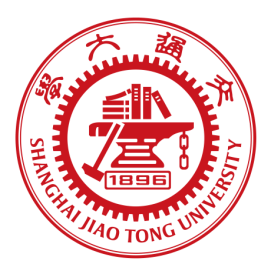
\includegraphics[width=5cm]  {fig1.png}} 
 \end{figure}

\begin{center}
\songti \zihao{-2} 上海交通大学学位论文
\end{center}
%该页为中文扉页。无需页眉页脚,纸质论文应装订在右侧
~\\
\begin{center}
\songti \zihao{1} \textbf{中法戏剧比较}
\end{center}
%中文论文标题,1行或2行,宋体,加粗,二号,居中。论文题目不得超过36个汉字
~\\
~\\
~\\
\begin{center}
\heiti \zihao{4}
\begin{tabular}{l}
\textbf{姓\quad 名:}王海诚\\
\textbf{学\quad 号:}519261910011\\
\textbf{导\quad 师:}Hui-Ling PROVOST\\
\textbf{学\quad 院:}巴黎卓越工程师学院 \\
\textbf{学科/专业名称:}法语(中法合作办学)\\
\textbf{申请学位层次:}学士\\
\end{tabular}
\end{center}
~\\
\begin{center}
\songti \zihao{4} \textbf{2023年05月}
\end{center}

\newpage
\thispagestyle{empty}
~\\
\begin{center}
\zihao{4}
\textbf{
A Dissertation Submitted to \\
Shanghai Jiao Tong University for Bachelor Degree}
\end{center}
~\\
\begin{center}
\zihao{-2}\textbf{
\MakeUppercase{Comparaison du Theatre entre la France et la Chine}}
\end{center}
%英文论文标题:大写,Times New Roman,加粗,14 points,居中
~\\
~\\
~\\
\begin{center}
\zihao{3} 
\textbf{Author:} Haicheng Wang \\
\textbf{Supervisor:} Hui-Ling PROVOST 
\end{center}
~\\
~\\
~\\
\begin{center}
\zihao{3} 
School of Paris Elite Institution  of Technology \\
Shanghai Jiao Tong University \\
Shanghai, P.R.China \\
May 11$^{\mathrm{th}}$, 2023
\end{center}

\newpage
\thispagestyle{empty}
\begin{center}
\heiti \zihao{3}\textbf{
上海交通大学\\
学位论文原创性声明}
\end{center}

\zihao{-4}
本人郑重声明:所呈交的学位论文,是本人在导师的指导下,独立进行研究工作所取得的成果。除文中已经注明引用的内容外,本论文不包含任何其他个人或集体已经发表或撰写过的作品成果。对本文的研究做出重要贡献的个人和集体,均已在文中以明确方式标明。本人完全知晓本声明的法律后果由本人承担。

\begin{flushright}
\begin{tabular}{l}
\zihao{4}
学位论文作者签名:\hspace{20mm}\qquad\\
\zihao{4}
日期:\qquad 年\qquad 月\qquad 日
\end{tabular}
\end{flushright}

~\\
\begin{center}
\heiti \zihao{3}\textbf{
上海交通大学\\
学位论文使用授权书}
\end{center}

本人同意学校保留并向国家有关部门或机构送交论文的复印件和电子版,允许论文被查阅和借阅。\\
本学位论文属于 :\par
□公开论文\par
□内部论文,保密□1年/□2年/□3年,过保密期后适用本授权书。\par
□秘密论文,保密\_\_\_年(不超过10年),过保密期后适用本授权书。\par
□机密论文,保密\_\_\_年(不超过20年),过保密期后适用本授权书。\par
(请在以上方框内选择打“√”)\\

\begin{flushright}
\zihao{4}
\begin{tabular}{l l}
学位论文作者签名:\hspace{10mm}\qquad \hspace{100mm}&指导教师签名:\qquad \\
日期:\qquad 年\qquad 月\qquad 日 &日期:\qquad 年\qquad 月\qquad 日\\
\end{tabular}
\end{flushright}

\newpage
\pagenumbering{Roman}
\fancyhead[LH]{上海交通大学学位论文}


\heiti \addcontentsline{toc}{section}{摘\quad 要}
\section*{摘\quad 要}
%摘要:二字间空一格,黑体16磅加粗居中,单倍行距,段前24磅,段后18磅。

\hspace{8mm}
\songti 本文介绍了法国和中国的戏剧历史、戏剧的相似和不同之处以及当前戏剧的状况。在第一章,文章概述了法国和中国戏剧的历史,包括中世纪、17、18、19和20世纪的法国戏剧以及唐、元、明、清和现代时期的中国戏剧,分析了包括莫里哀、雨果和贝克特在内的多位著名法国戏剧作家与关汉卿等数位中国古代戏剧家的创作特点。第二章探讨了法国和中国戏剧之间的差异和相似之处,如文化背景、舞台表演、剧本结构和传统服饰等,并进行了详尽的描述。第三章通过具体的示例,分析了戏剧的形成,包括宗教、历史、文化和地理方面的因素,结合之前的内容进行深入解析。最后一章则主要讨论了法国和中国戏剧的现状,以及为戏剧保护提出的建议。总体而言,本文突出了中法两国戏剧的丰富性和多样性,同时也探讨了两国之间的共性和差异。 通过对历史和文化因素的分析,本文对两国戏剧的形成和演变以及当今戏剧的现状提供了深刻的见解。 最后,本文强调了保护和促进戏剧作为一种重要的艺术表现形式和文化遗产的重要性。\\
\\
\songti \textbf{关键词}:中法戏剧, 中法文化, 中法历史, 表演艺术, 戏剧比较\\
%关键字:宋体12磅,行距20磅,段前段后0磅,关键字之间用逗号隔开,关键词三个字加粗。

\newpage
\addcontentsline{toc}{section}{ABSTRACT}
\section*{ABSTRACT}
%ABSTRCT:Arial 16磅加粗居中,单倍行距,段前24磅,段后18磅

\hspace{8mm}
%英文摘要内容:Times New Roman 12磅,行距20磅段前段后0磅
This thesis provides an overview of the history and current state of theater in France and China, exploring the similarities and differences between the two countries. Chapter I provides a brief history of theater in France and China, covering different periods from the medieval era to the modern age. The chapter also highlights the key features of each period and its impact on the development of theater in both countries. For instance, the theater of the 17th century in France was marked by the works of Molière and the Commedia dell'arte, while the theater of the Tang dynasty in China saw the emergence of various forms of Chinese opera.
Chapter II examines the differences and similarities between French and Chinese theater. Despite the differences in cultural traditions and styles of performance, there are similarities between the two countries. For example, both French and Chinese theater incorporate elements of music, dance, and poetry to create a spectacle that captivates the audience. However, there are also significant differences, such as the structure and the personal character.
Chapter III analyzes the formation of theater in France and China, exploring the historical, religious, cultural, and geographic factors that contributed to the development of theater in each country. The chapter also provides a small example to illustrate the evolution of theater in both countries. Religion played a significant role in the development of theater in both countries, with religious ceremonies and festivals often serving as the basis for early theatrical performances.
Chapter IV examines the current state of theater in France and China, providing an overview of the different types of theater productions and trends in each country. The chapter concludes with a proposal for the preservation and promotion of theater in both countries.
Overall, this thesis highlights the richness and diversity of theater in France and China, while also exploring the commonalities and differences between the two countries. Through an analysis of historical and cultural factors, the thesis provides insights into the formation and evolution of theater in both countries, as well as the current situations of theater today. Ultimately, the thesis emphasizes the importance of preserving and promoting theater as a vital form of artistic expression and cultural heritage.\\ 
~\\
\textbf{Key words}: chinese/french theater, chinese/french history, chinese/french culture, performing art \\
%Keywords:Times New Roman 12磅,行距20磅, “key words” 两词加粗

\newpage
\addcontentsline{toc}{section}{RESUME}
\section*{RESUME}
\hspace{8mm}
%%ABSTRCT:Arial 16磅加粗居中,单倍行距,段前24磅,段后18磅
%Ce document aborde l'histoire du théâtre en France et en Chine, ainsi que les différences et les similitudes entre ces deux cultures. Le premier chapitre de ce document offre un aperçu de l'histoire du théâtre, en commençant par l'histoire du théâtre français, qui remonte au Moyen Âge. On explore les périodes clés du théâtre français, notamment le 17ème siècle, le 18ème siècle, le 19ème siècle et le 20ème siècle. Le deuxième chapitre se concentre sur l'histoire du théâtre chinois, en remontant à la dynastie Tang et en explorant les périodes suivantes jusqu'à l'époque moderne. on examine les différents styles de théâtre chinois et les événements historiques qui ont influencé leur développement. Dans le troisième chapitre, on examine les facteurs qui ont influencé la formation du théâtre, tels que l'aspect religieux, historique, culturel et géographique. En se basant sur un exemple précis, on montre comment ces facteurs ont contribué à la création et à l'évolution du théâtre. Le quatrième chapitre examine l'état actuel du théâtre en France et en Chine. On discute de la popularité du théâtre dans ces deux pays, ainsi que de l'état actuel de l'industrie du théâtre dans chaque pays. Enfin, l'auteur propose des idées pour améliorer la préservation et la promotion du théâtre. L'ensemble du mémoire se concentre sur les différences et les similitudes entre le théâtre français et chinois. Le deuxième chapitre examine les différences dans les styles de théâtre, tels que le théâtre classique français et le théâtre chinois d'ombres. Le deuxième chapitre examine également les similitudes, telles que la façon dont le théâtre a été utilisé pour transmettre des histoires et des traditions culturelles. En fin de compte, ce mémoire offre une introduction complète à l'histoire et à la culture du théâtre en France et en Chine. En explorant les similitudes et les différences entre ces deux cultures, on offre une perspective unique sur l'histoire du théâtre et sa signification dans le monde d'aujourd'hui. Ce mémoire pourrait être utile pour ceux qui cherchent à mieux comprendre les différences et les similitudes entre les cultures françaises et chinoises.\\
Cette thèse offre une vue d'ensemble de l'histoire et de l'état actuel du théâtre en France et en Chine, explorant les similitudes et les différences entre les deux pays. Le chapitre I offre un aperçu de l'histoire du théâtre, en commençant par l'histoire du théâtre français, qui remonte au Moyen Âge. On explore les périodes clés du théâtre français, notamment le 17ème siècle, le 18ème siècle, le 19ème siècle et le 20ème siècle.. Le chapitre met également en évidence les caractéristiques clés de chaque période et leur impact sur le développement du théâtre dans les deux pays. Par exemple, le théâtre du XVIIe siècle en France a été marqué par les œuvres de Molière et de la Commedia dell'arte, tandis que le théâtre de la dynastie Tang en Chine a vu l'émergence de diverses formes d'opéra chinois.
Le chapitre II examine les différences et les similitudes entre le théâtre français et chinois. Malgré les différences de traditions culturelles et de styles de présentation, il existe des similitudes entre les deux pays. Par exemple, le théâtre français et chinois incorpore des éléments de musique, de danse et de poésie pour créer un spectacle qui captive le public. Cependant, il y a également des différences significatives, telles que les costumes et le style du jeu.
Le chapitre III analyse la formation du théâtre en France et en Chine, explorant les facteurs historiques, religieux, culturels et géographiques qui ont contribué au développement du théâtre dans chaque pays. Le chapitre fournit également un petit exemple pour illustrer l'évolution du théâtre dans les deux pays. La religion a joué un rôle important dans le développement du théâtre dans les deux pays, les cérémonies et festivals religieux servant souvent de base aux premières représentations théâtrales.
Le chapitre IV examine l'état actuel du théâtre en France et en Chine, en offrant un aperçu des différents types de productions théâtrales et des tendances dans chaque pays. Le chapitre conclut par une proposition pour la préservation et la promotion du théâtre dans les deux pays.
Dans l'ensemble, cette thèse met en évidence la richesse et la diversité du théâtre en France et en Chine, tout en explorant les similitudes et les différences entre les deux pays. À travers une analyse des facteurs historiques et culturels, la thèse offre des opinions sur la formation et l'évolution du théâtre dans les deux pays, ainsi que sur la situation actuelle du théâtre aujourd'hui. En fin de compte, la thèse souligne l'importance de préserver et de promouvoir le théâtre en tant que forme d'expression artistique et patrimoine culturel essentiels.\\
%英文摘要内容:Times New Roman 12磅,行距20磅段前段后0磅
~\\
\textbf{Mots clés}: théâtre chinois/français, comparaison du théâtre, histoire chinoise/française, culture chinoise/française 

\newpage
\renewcommand\contentsname{\MakeUppercase{\textbf{Table des Matieres}}}


\begin{center}
{\tableofcontents
\thispagestyle{fancy}
\fancyhead[LH]{上海交通大学学位论文}
}
\end{center}

\emergencystretch 1em
\newpage
\fancyhead[LH]{上海交通大学学位论文}
\fancyhead[RH]{Introduction}
\pagenumbering{arabic}
\addcontentsline{toc}{section}{Introduction}
\section*{Introduction}
%\subsection{Avant-propos}
%L'art du théâtre est une forme d'expression artistique qui a traversé les siècles et les cultures. Il est un mélange de littérature et de représentation qui peut refléter la culture, l'histoire et même les valeurs d'une nation. Le théâtre est un art millénaire qui a évolué différemment selon les pays et les époques. Dans ce mémoire, nous nous concentrerons sur les similitudes et les différences entre le théâtre chinois et le théâtre français, ainsi que sur les raisons historiques et culturelles de leur formation. Nous explorerons comment la culture et l'histoire ont influencé la forme du théâtre dans ces deux pays. Le théâtre français et le théâtre chinois sont deux formes d'art très différentes, mais qui ont chacune leur propre richesse et leur propre histoire. Le théâtre français a une longue tradition qui remonte à l'Antiquité grecque, tandis que le théâtre chinois a une histoire qui remonte à plus de deux mille ans. Les deux formes d'art ont évolué différemment en fonction de leur contexte historique et culturel. Dans ce mémoire, nous analyserons le développement du théâtre français et chinois, en examinant leurs caractéristiques et les contextes historiques dans lesquels ils ont évolué. Nous comparerons également leurs techniques et styles, en explorant les différences et les similitudes entre ces deux formes d'art. Nous utiliserons des méthodes variées pour analyser le développement du théâtre dans ces deux pays, et les résultats attendus sont une meilleure compréhension des similitudes et des différences entre ces deux formes d'art. Ce mémoire vise à contribuer à une meilleure compréhension et appréciation du théâtre français et chinois, ainsi qu'à la promotion de la compréhension interculturelle et de la préservation des traditions théâtrales. Nous espérons que cette recherche permettra aux générations futures de mieux comprendre et apprécier cet art millénaire.
%\subsection{Les Sujets Etudiés}
\hspace{8mm}
Le théâtre est une forme d'art qui combine la littérature et la représentation sur scène avec des comédiens, reflétant ainsi la culture, l'histoire et les valeurs d'une nation. En France, le théâtre a une longue histoire qui remonte à l'époque romaine, et a connu de nombreuses évolutions au fil des siècles. En Chine, le théâtre est un art également très ancien, et a été influencé par de nombreuses traditions culturelles différentes. Bien que le théâtre en France et en Chine aient des racines historiques respectivement, il existe des différences marquées entre les deux formes d'art en termes de style, de contenu et de technique. En France, le théâtre est souvent considéré comme un art élitiste, avec des pièces qui sont souvent écrites par des auteurs célèbres et jouées dans des théâtres prestigieux. Le contenu des pièces de théâtre en France peut être très varié, allant de la comédie légère à la tragédie en passant par la satire politique. En Chine, le théâtre est considéré comme un art populaire, et les pièces sont souvent jouées dans des théâtres de rue ou sur les scènes, parfois provisoires, dans des parcs publics. Le contenu des pièces de théâtre en Chine est généralement axé sur les traditions culturelles et les croyances, avec des légendes qui sont souvent empreintes de symbolisme et de moralité. Côté esthétique, le théâtre chinois utilise également des techniques telles que la danse, la musique et les arts martiaux pour raconter des histoires, ce qui le rend très différent du théâtre en France. Dans ce mémoire, nous nous concentrerons sur les similitudes et les différences entre le théâtre chinois et le théâtre français, ainsi que sur les raisons historiques et culturelles de leur formation. La question centrale que nous chercherons à répondre est la suivante : comment la culture et l'histoire influencent-elles la forme du théâtre ? Tout d'abord, nous introduirons le processus de développement du théâtre français et chinois, en analysant leurs caractéristiques et les contextes historiques. Pour introduire l'histoire du théâtre français, nous distinguerons les différentes époques accompagnées des œuvres représentatives telles que le baroque avec avec des pièces de Corneille, Jean Racine, Molière, le siècle des lumières avec celles de Voltaire, Dumas, Diderot, le dramaturge du romantisme Victor Hugo et enfin Beckett représentera l'existentialisme du XXème siècle, notamment pendant la Seconde Guerre mondiale. En analysant ces œuvres et leurs auteurs de chaque époque, nous pourrons résumer leurs caractéristiques et leurs liens avec le contexte historique. Sachant que le théâtre français et le théâtre chinois sont bien différents, nous les comparerons et donnerons des pistes pour illustrer leur distinction par la suite. Par exemple, le théâtre français a hérité principalement de la forme tragi-comique de la Grèce antique. Il contient parfois un ton ironique, ou exprime les pensées de l'auteur sur les phénomènes sociaux. En Chine, le théâtre était initialement introduit par les familles impériales pour leurs distractions et des célébrations. Par la suite, devenant un art populaire du folk, il se consacre à l'adaptation d'événements historiques ou au récit d'une histoire d'amour et s'efforce de lui donner une fin heureuse parce que les Chinois aiment bien une fin positive et détestent une fin tragique. Aussi en termes de technique, différentes théories et les contextes historiques et culturels pour trouver une loi derrière la formation du théâtre. En fin de compte, nous conclurons sur les relations entre la formation du théâtre et la culture et l'histoire. Les sujets étudiés dans ce mémoire sont donc le théâtre chinois et le théâtre français, ainsi que leurs similitudes et leurs différences. Nous analyserons également les contextes historiques et culturels qui ont influencé leur formation, ainsi que les caractéristiques et les techniques propres à chaque forme de théâtre. Enfin, nous chercherons à trouver une loi derrière la formation du théâtre en combinant différentes théories et en examinant les contextes historiques et culturels. La recherche sur la comparaison du théâtre entre la France et la Chine a donc pour but d'explorer les différences et les similitudes entre ces deux formes d'art. Cela peut aider à mieux comprendre les racines culturelles et historiques du théâtre dans ces deux pays, ainsi que les influences qui ont contribué à façonner leur style et leur contenu.La recherche pourrait également permettre de mieux apprécier les différences entre les techniques utilisées dans le théâtre en France et en Chine, et d'en apprendre davantage sur la façon dont ces deux formes d'art évoluent et se développent. En comprenant les différences et les similitudes entre le théâtre en France et en Chine, on peut mieux apprécier la richesse et la diversité de ces deux formes d'art.

En somme, la recherche sur le théâtre en France et en Chine est d'une grande importance pour mieux comprendre les différences et les similitudes entre ces deux formes d'art, ainsi que pour favoriser la compréhension et le respect entre les cultures. Elle peut également contribuer à la préservation et à la transmission des traditions théâtrales en France et en Chine, pour que les générations futures puissent continuer à apprécier cet art millénaire. Ces connaissances pourront être utiles pour les étudiants en théâtre, les chercheurs en histoire et culture, ainsi que pour les professionnels du théâtre qui souhaitent mieux comprendre les différentes formes de théâtre à travers le monde.


\newpage
\fancyhead[LH]{上海交通大学学位论文}
\fancyhead[RH]{Chapitre I Aperçu de L'histoire du Théâtre} \label{sec:1}
%\pagenumbering{arabic}
\section{Aperçu de L'histoire du Théâtre}
\hspace{8mm}
Le théâtre est une forme d'art qui a traversé les siècles et qui continue de captiver les spectateurs du monde entier. Depuis les tragédies grecques jusqu'aux pièces contemporaines, le théâtre a évolué pour devenir une expression artistique complexe et multidimensionnelle. Il combine le texte, la narration, la musique, la danse et la mise en scène pour créer une expérience immersive pour le public. Le théâtre est un art vivant qui permet aux acteurs de donner vie aux personnages et aux histoires, créant ainsi une connexion émotionnelle avec le public. Les pièces de théâtre peuvent être comiques, dramatiques, romantiques, satiriques ou politiques, et elles peuvent aborder des thèmes universels tels que l'amour, la mort, la justice, la liberté et la condition humaine. Le théâtre est également un art collaboratif qui implique de nombreux professionnels tels que les acteurs, les metteurs en scène, les décorateur-scénographes, les costumiers, les éclairagistes et les musiciens. Chaque élément de la production contribue à créer une atmosphère unique et à donner vie à l'histoire racontée sur scène. Enfin, le théâtre est un art qui peut être apprécié par tous, indépendamment de l'âge, de la culture ou de la langue. Les pièces de théâtre sont souvent traduites et adaptées pour être présentées dans différentes régions du monde, permettant ainsi aux spectateurs de découvrir de nouvelles cultures et de nouvelles perspectives. 
En bref, le théâtre est une forme d'art riche et diversifiée qui continue de fasciner et d'inspirer les gens du monde entier. Que ce soit pour divertir, éduquer ou provoquer une réflexion, le théâtre est un moyen puissant de communiquer des idées et des émotions, et de créer une expérience inoubliable pour le public. Dans ce mémoire, nous nous intéressons à l'histoire du théâtre français et chinois, donc dans la partie suivante nous les introduirons respectivement.

\subsection{Brève Histoire du Théâtre Français}

Le théâtre occidental trouve ses racines dans la Grèce antique, où les représentations théâtrales étaient un élément important de la vie culturelle. Les pièces de théâtre étaient jouées dans des théâtres en plein air, tels que le théâtre de Dionysos à Athènes, et étaient souvent des tragédies ou des comédies. Les pièces étaient écrites et jouées pour célébrer les dieux et les héros de la mythologie grecque, et pour explorer des thèmes tels que la justice, la vengeance et la destinée. Les acteurs portaient des masques pour représenter différents personnages et les pièces étaient accompagnées de musique et de danse. Le théâtre grec a eu une influence durable sur le théâtre occidental, en particulier sur la tragédie et la comédie, et continue d'être étudié et apprécié pour son importance historique et culturelle. C'est aussi la source d'inspiration de longue date du théâtre français. 

Le théâtre français a une longue et riche histoire qui remonte à l'époque médiévale. Au Moyen Âge, les spectacles étaient souvent présentés dans les églises et les places publiques, et étaient principalement des représentations religieuses. Au fil du temps, le théâtre a évolué pour inclure des pièces profanes et des comédies. Au 17ème siècle, le théâtre français a connu un âge d'or avec l'avènement de la Comédie-Française, qui est toujours en activité aujourd'hui. Les pièces de Molière, Racine et Corneille ont été présentées pour la première fois à cette époque et sont toujours considérées comme des classiques du théâtre français. Au 18ème siècle, le théâtre français a connu une période de déclin, mais a été revitalisé au 19ème siècle avec l'avènement du romantisme. Les pièces de Victor Hugo, Alexandre Dumas fils et Eugène Scribe ont été présentées pour la première fois à cette époque. Au 20ème siècle, le théâtre français a continué à évoluer avec l'avènement du théâtre de l'absurde et du nouveau théâtre réaliste. Des dramaturges tels que Samuel Beckett, Jean Genet et Eugène Ionesco ont été présentés pour la première fois à cette époque. Aujourd'hui, le théâtre français continue d'être un élément important de la culture française, avec de nombreuses productions présentées chaque année à travers le pays. Dans la partie suivante, nous detaillerons les caractéristiques particulière de chaque époque.\\
\subsubsection{Théâtre du Moyen Âge (Ve-XVe siècle)}
Le théâtre français au Moyen Âge était principalement représenté dans les églises et les places publiques\mycite{mazouer2016theatre}. Les spectacles étaient souvent des représentations religieuses, telles que des mystères et des miracles, qui racontaient des histoires bibliques et des vies de saints. Les acteurs étaient souvent des membres du clergé ou des laïcs locaux. Les mystères étaient des pièces qui racontaient des histoires de la Bible, tandis que les miracles étaient des pièces qui racontaient des histoires de saints et de miracles. Les spectacles étaient souvent accompagnés de musique et de chants, et étaient présentés en latin ou en français. Les mystères étaient souvent présentés en plusieurs parties, chacune représentant une histoire différente de la Bible. Les acteurs portaient des costumes élaborés et des masques pour représenter les différents personnages. Les spectacles étaient souvent présentés sur des chariots ou des plateformes mobiles, qui étaient déplacés d'un endroit à l'autre pour permettre à un plus grand nombre de personnes d'assister aux représentations. Les miracles étaient souvent présentés sous forme de pièces courtes, qui racontaient des histoires de saints et de miracles. Les acteurs utilisaient souvent des accessoires tels que des bâtons et des bannières pour représenter les différents personnages. Au fil du temps, le théâtre français a évolué pour inclure des pièces profanes et des comédies. Les pièces profanes étaient souvent des farces, qui étaient des pièces courtes et comiques qui se moquaient de la société et de ses travers. Les comédies étaient des pièces plus élaborées qui racontaient des histoires d'amour et de tromperie. Le théâtre français au Moyen Âge était donc principalement religieux, mais a évolué pour inclure des pièces profanes et des comédies. Cette évolution a jeté les bases du théâtre français moderne, qui est toujours un élément important de la culture française. aujourd'hui. Un exemple est donné ci-dessus pour l'illustrer ces caractéristiques.
\begin{figure}[H] 
\center{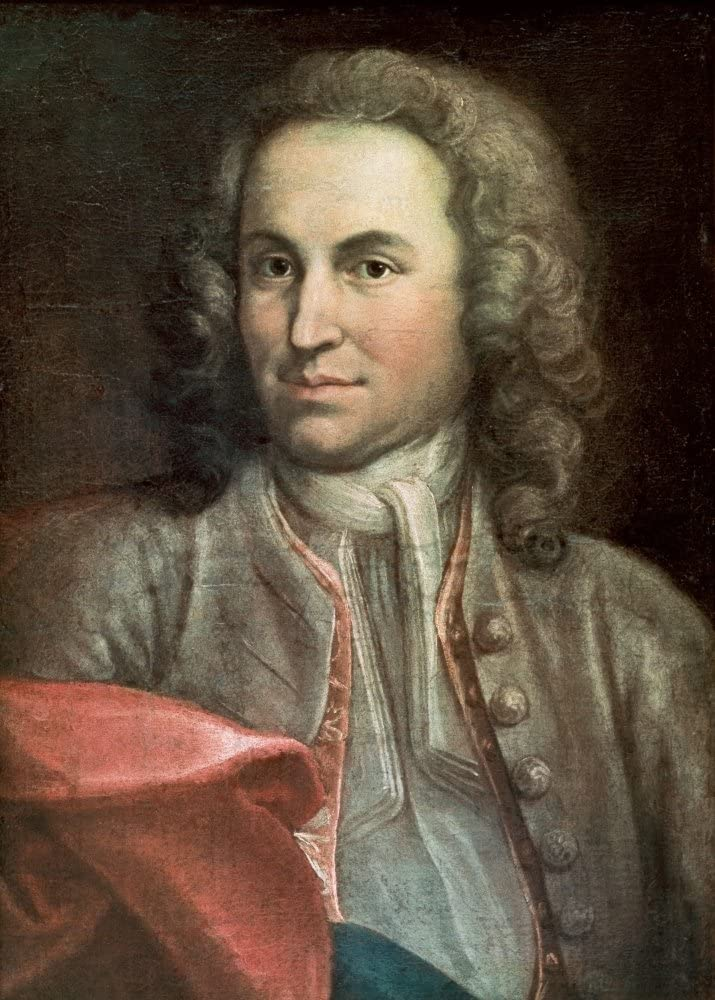
\includegraphics[width=0.4\textwidth]{Adam.jpg}} 
\caption{Le portrait de Adam de la Halle (1220-1288)}
\end{figure}
Adam de la Halle était un poète et dramaturge français du XIIIe siècle. Il est considéré comme l'un des plus grands auteurs de théâtre du Moyen Âge et est surtout connu pour ses pièces de théâtre profanes telles que ``Le Jeu de Robin et Marion" et ``Le Jeu de la Feuillée"\mycite{huot1987transformations}. ``Le Jeu de Robin et Marion" est considéré comme la première pièce de théâtre française profane. Elle a été écrite en langue vernaculaire française et a été présentée pour la première fois devant des publics laïcs. La pièce raconte l'histoire d'amour entre Robin, un berger, et Marion, une bergère, et est considérée comme une comédie pastorale. ``Le Jeu de la Feuillée" est une autre pièce de théâtre profane écrite par Adam de la Halle. Elle raconte l'histoire d'un groupe de jeunes gens qui se rendent dans une forêt pour célébrer la fête de la Saint-Nicolas. La pièce est considérée comme une comédie et est souvent comparée à ``Le Jeu de Robin et Marion". Adam de la Halle a également écrit des chansons et des poèmes, ainsi que des pièces de théâtre religieuses. Il a été influencé par les troubadours et les trouvères, et a utilisé la musique et la poésie pour raconter des histoires dans ses pièces de théâtre. 

\subsubsection{Théâtre du 17ème Siècle}
Le théâtre français au 17ème siècle, également connu sous le nom de théâtre classique, est considéré comme l'âge d'or du théâtre français, avec des pièces qui ont influencé le théâtre européen pendant des siècles. Il est caractérisé par des règles strictes et des normes de représentation qui ont été établies par les dramaturges les plus célèbres de l'époque, tels que Corneille, Racine et Molière\mycite{rambert1861corneille}. Ce théâtre a été influencé par les idées de l'humanisme et de la Renaissance, ainsi que par les mouvements artistiques de l'époque, tels que le classicisme et le baroque\mycite{attinger1981esprit}.

Les pièces de théâtre étaient généralement écrites en vers alexandrins et suivaient la structure de la tragédie classique, qui était divisée en cinq actes. Les personnages étaient souvent des figures historiques ou mythologiques et les intrigues étaient centrées sur des conflits moraux et éthiques. Les thèmes fréquents comprenaient la passion, la vengeance, la trahison, la justice et l'amour\mycite{despois1874theatre}.

Les pièces étaient jouées sur des scènes relativement simples, avec des décors minimalistes et des costumes extravagants. Les acteurs étaient tenus de suivre un ensemble de règles strictes en ce qui concerne leur comportement sur scène, leur diction et leur gestuelle. Les acteurs devaient également suivre un ensemble de règles de jeu, appelées ``les règles du jeu", qui exigeaient un comportement et une présentation spécifiques sur scène\mycite{forestier1996theatre}.
Le théâtre français du 17ème siècle a connu un grand succès, en grande partie grâce aux talents de dramaturges tels que Corneille, Racine et Molière, qui ont créé des pièces qui étaient à la fois divertissantes et éducatives. Nous donnerons Molière comme l'exemple.
\begin{figure}[H] 
\center{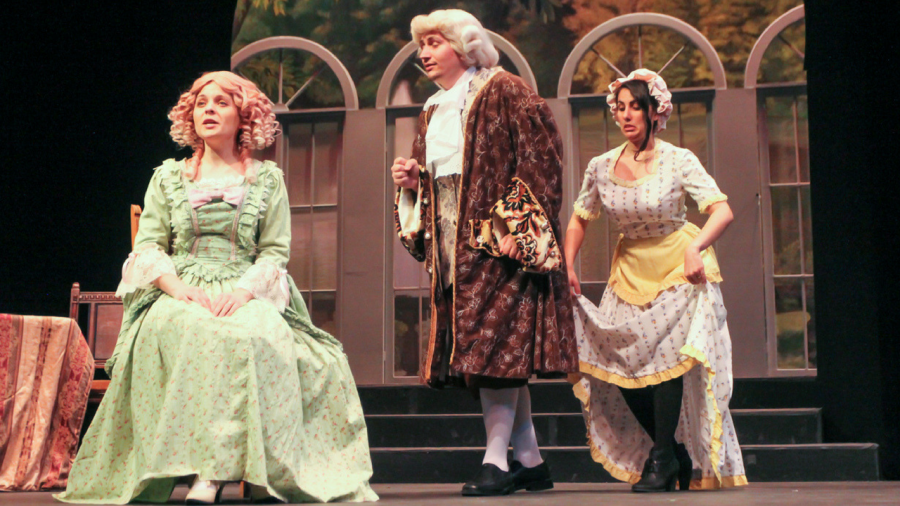
\includegraphics[width=0.95\textwidth]{tartuffeplay.png}} 
\caption{Une scène du drame ``Tartuffe"}
\end{figure}

\begin{figure}[H] 
\center{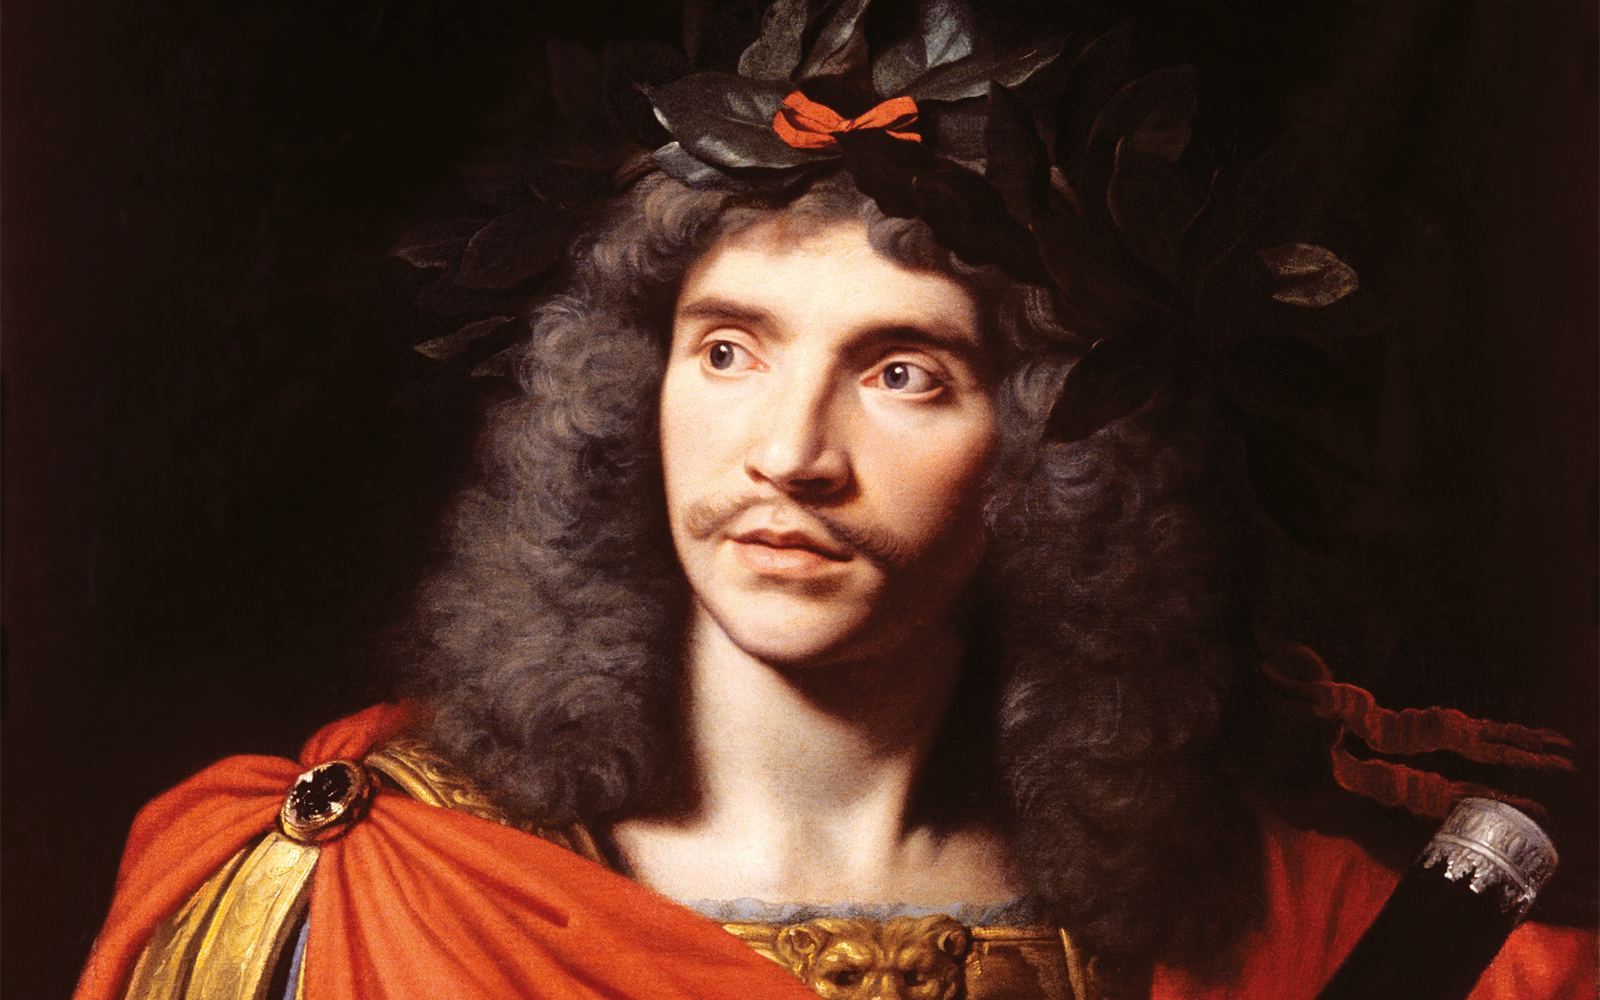
\includegraphics[width=0.95\textwidth]{moliere.jpg}} 
\caption{Le portrait de Molière (1622-1673)}
\end{figure}
Les œuvres de Molière sont des comédies de mœurs satiriques, caractérisées par un style comique, une langue française élégante et une caractérisation complexe des personnages. Les pièces de Molière ont souvent pour sujet les comportements et les travers de la société de son temps, en particulier de la bourgeoisie. Ses personnages sont souvent caricaturaux, tels que le bourgeois arrogant, le médecin ignorant ou le dévot hypocrite\mycite{gaines1984social}. Il dénonce les comportements ridicules et les préjugés de son temps, tels que la manie des maris jaloux ou l'obsession de la noblesse pour les titres. Le style de Molière est caractérisé par une grande vivacité et un sens aigu de l'observation. Ses personnages sont souvent dotés d'une répartie spirituelle et de jeux de mots, et les scènes sont rythmées par des quiproquos et des rebondissements comiques. Molière est également célèbre pour la complexité de ses personnages, qui sont souvent ambigus et contradictoires. Ses personnages ont des motivations et des émotions complexes, et leur évolution au cours de la pièce est souvent surprenante.

\subsubsection{Théâtre du 18ème Siècle}
Le théâtre français du 18ème siècle a été marqué par un certain nombre de changements significatifs qui ont eu un impact sur l'ensemble de l'art théâtral. Au cours de cette période, le théâtre est devenu un véritable art populaire et a évolué pour devenir une forme d'expression culturelle qui a eu un impact sur la société française dans son ensemble. Au 18ème siècle, le théâtre français a été marqué par une grande diversité de genres, tels que la tragédie, la comédie, le drame bourgeois, le vaudeville et l'opéra-comique. Chaque genre avait ses propres caractéristiques et conventions, et était destiné à un public différent. Le public du théâtre français au 18ème siècle était très diversifié. Les représentations étaient souvent visitées par la noblesse française, les membres de la cour, les bourgeois et les travailleurs. Le théâtre était devenu un lieu où les gens de différentes classes sociales pouvaient se rassembler et partager des expériences culturelles. D'ailleurs, émergence de grands auteurs de théâtre français tels que Voltaire, Beaumarchais et Diderot ont apporté de nouvelles idées et ont remis en question les normes sociales de l'époque à travers leurs pièces, qui a eu un impact important sur la société française\mycite{carlson1998voltaire}. Les pièces de théâtre ont été utilisées pour critiquer les normes sociales et politiques de l'époque, et pour promouvoir de nouvelles idées. Le théâtre était également un lieu de divertissement et de rassemblement, offrant aux gens une évasion de la vie quotidienne.
\subsubsection{Théâtre du 19ème Siècle}
Le théâtre français du 19ème siècle est une période marquante de l'histoire culturelle de la France, qui a vu l'émergence de nombreux courants artistiques et théâtraux importants. Au 19ème siècle, la France traverse une période de profonds bouleversements politiques, économiques et sociaux. La Révolution française de 1789 a entraîné des changements radicaux dans la vie politique, économique et sociale du pays. Le 19ème siècle est également marqué par les guerres napoléoniennes, l'essor de l'industrialisation, l'urbanisation et la croissance démographique. Ces changements ont eu une influence sur le théâtre français, qui a été le reflet des préoccupations et des aspirations de la société de l'époque.
Le théâtre français du 19ème siècle a connu de nombreux courants théâtraux importants,qui ont souvent exploré les relations humaines, la politique, la morale, l'amour et la mort:
\begin{enumerate}
\item Le romantisme : Le romantisme a été un mouvement important dans le théâtre français, avec des thèmes tels que l'amour impossible, la nature, l'histoire et la révolution. Il se caractérise par une sensibilité à la nature, à l'émotion et à l'individu. Au théâtre, les pièces romantiques mettent en scène des héros passionnés, souvent tragiques, confrontés à des situations dramatiques. Victor Hugo est l'un des plus grands représentants du romantisme au théâtre.

\item Le réalisme : Le réalisme est un courant artistique qui a émergé dans la seconde moitié du 19ème siècle. Au théâtre, les pièces réalistes se caractérisent par leur représentation fidèle de la vie quotidienne, sans idéalisation ni embellissement. Les auteurs réalistes cherchent à rendre compte des problèmes sociaux de leur époque. Émile Zola est l'un des plus grands représentants du réalisme au théâtre.

\item Le symbolisme : Le symbolisme est un courant artistique qui se développe à la fin du 19ème siècle. Au théâtre, les pièces symbolistes mettent en scène des personnages en quête de spiritualité, confrontés à des situations énigmatiques. Le symbolisme se caractérise par l'utilisation de symboles, de métaphores et de suggestions plutôt que par une représentation réaliste de la vie. Maurice Maeterlinck est l'un des plus grands représentants du symbolisme au théâtre.
\end{enumerate}

Les personnages du théâtre français du 19ème siècle étaient souvent des représentations stéréotypées de différents types sociaux et professionnels. Les comédies ont souvent présenté des personnages de la bourgeoisie, tandis que les tragédies ont mis en scène des rois et des reines. Les personnages féminins ont également été développés, avec des rôles forts et indépendants. En plus, des innovations techniques ont permis des avancées importantes dans la production théâtrale. Les décors ont été améliorés avec l'introduction de l'éclairage au gaz et des machines pour les changements de scène. Les acteurs ont également été mieux formés et ont développé des techniques de jeu plus subtiles.
\begin{figure}[H] 
\center{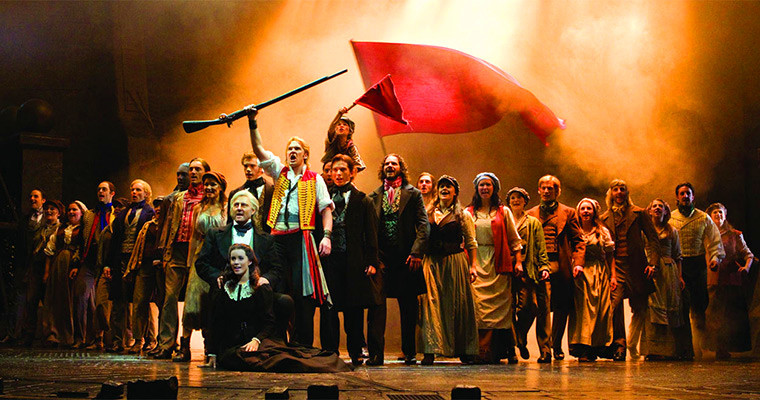
\includegraphics[width=0.95\textwidth]{miserable.jpg}} 
\caption{Une scène du drame ``Les Misérables"}
\end{figure}

\begin{figure}[H] 
\center{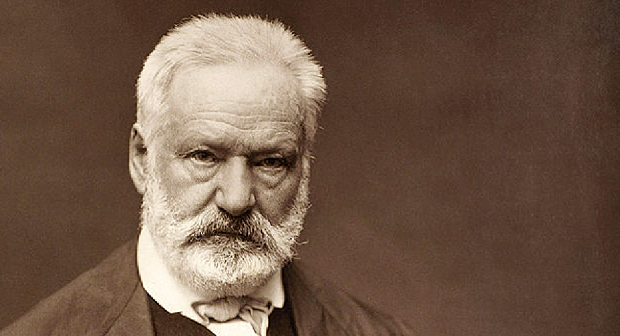
\includegraphics[width=0.8\textwidth]{hugo.png}} 
\caption{Le portrait de Victor Hugo (1802-1885)}
\end{figure}
  Victor Hugo est considéré comme l'un des plus grands écrivains de langue française et ses œuvres ont marqué la littérature française du XIXe siècle. Hugo est connu pour son style d'écriture poétique, expressif et lyrique. Il utilise souvent des images fortes et des métaphores pour créer une atmosphère intense et émotionnelle. Son style est également caractérisé par une utilisation abondante de l'antithèse et du contraste. Les thèmes des œuvres de Victor Hugo sont variés et touchent à des sujets tels que la justice sociale, la révolte contre l'oppression, la liberté, l'amour et la mort\mycite{abc}. Hugo a également traité de sujets politiques et sociaux contemporains de son époque, tels que la monarchie, la Révolution française et la pauvreté. Les personnages de Hugo sont souvent complexes et profondément développés. Ils sont souvent confrontés à des dilemmes moraux difficiles et sont présentés avec une grande empathie et une compréhension psychologique. Hugo était un fervent défenseur de la justice sociale et ses œuvres sont imprégnées de cet engagement. Ses romans tels que ``Les Misérables" et ``Quatre-Vingt-Treize" dénoncent la pauvreté et l'injustice sociale et appellent à des changements politiques et sociaux. Il existe aussi des oeuvres caractérisées par une dimension épique, avec des scènes grandioses et dramatiques. Les récits épiques tels que ``Les Misérables"\mycite{hugo1863miserables} ou ``Notre-Dame de Paris"\mycite{hugo1904notre} sont ponctués de moments de bravoure, de combats et de sacrifices héroïques.

\subsubsection{Théâtre du 20ème Siècle}
Le théâtre français du 20ème siècle se caractérise par une grande diversité de styles et de mouvements artistiques, ainsi que par une profonde réflexion sur les enjeux politiques, sociaux et culturels de l'époque. Nous présenterons les plus typiques d'entre eux ci-dessous:
\begin{enumerate}
\item Le surréalisme : mouvement artistique et littéraire qui prône la libération de l'imagination et du subconscient, le surréalisme a eu une forte influence sur le théâtre français du 20ème siècle.

\item Le théâtre de l'absurde : en réaction à la Seconde Guerre mondiale et à l'échec de la société à empêcher cette catastrophe. Il est caractérisé par une rupture avec les conventions théâtrales traditionnelles, le théâtre de l'absurde se concentre sur l'absurdité et l'irrationnel de la condition humaine. Les œuvres de Samuel Beckette sont considérées comme les plus représentatives de ce courant.

\item Le théâtre politique : Dans les années 60 et 70, de nombreux artistes ont utilisé le théâtre pour exprimer leur engagement politique et leur opposition aux régimes autoritaires en place\mycite{bradby1990theatre}. Des compagnies comme le Théâtre du Soleil et la Comédie-Française ont produit des pièces qui critiquent la guerre, le colonialisme et l'injustice sociale.
\end{enumerate}
\begin{figure}[htb] 
\center{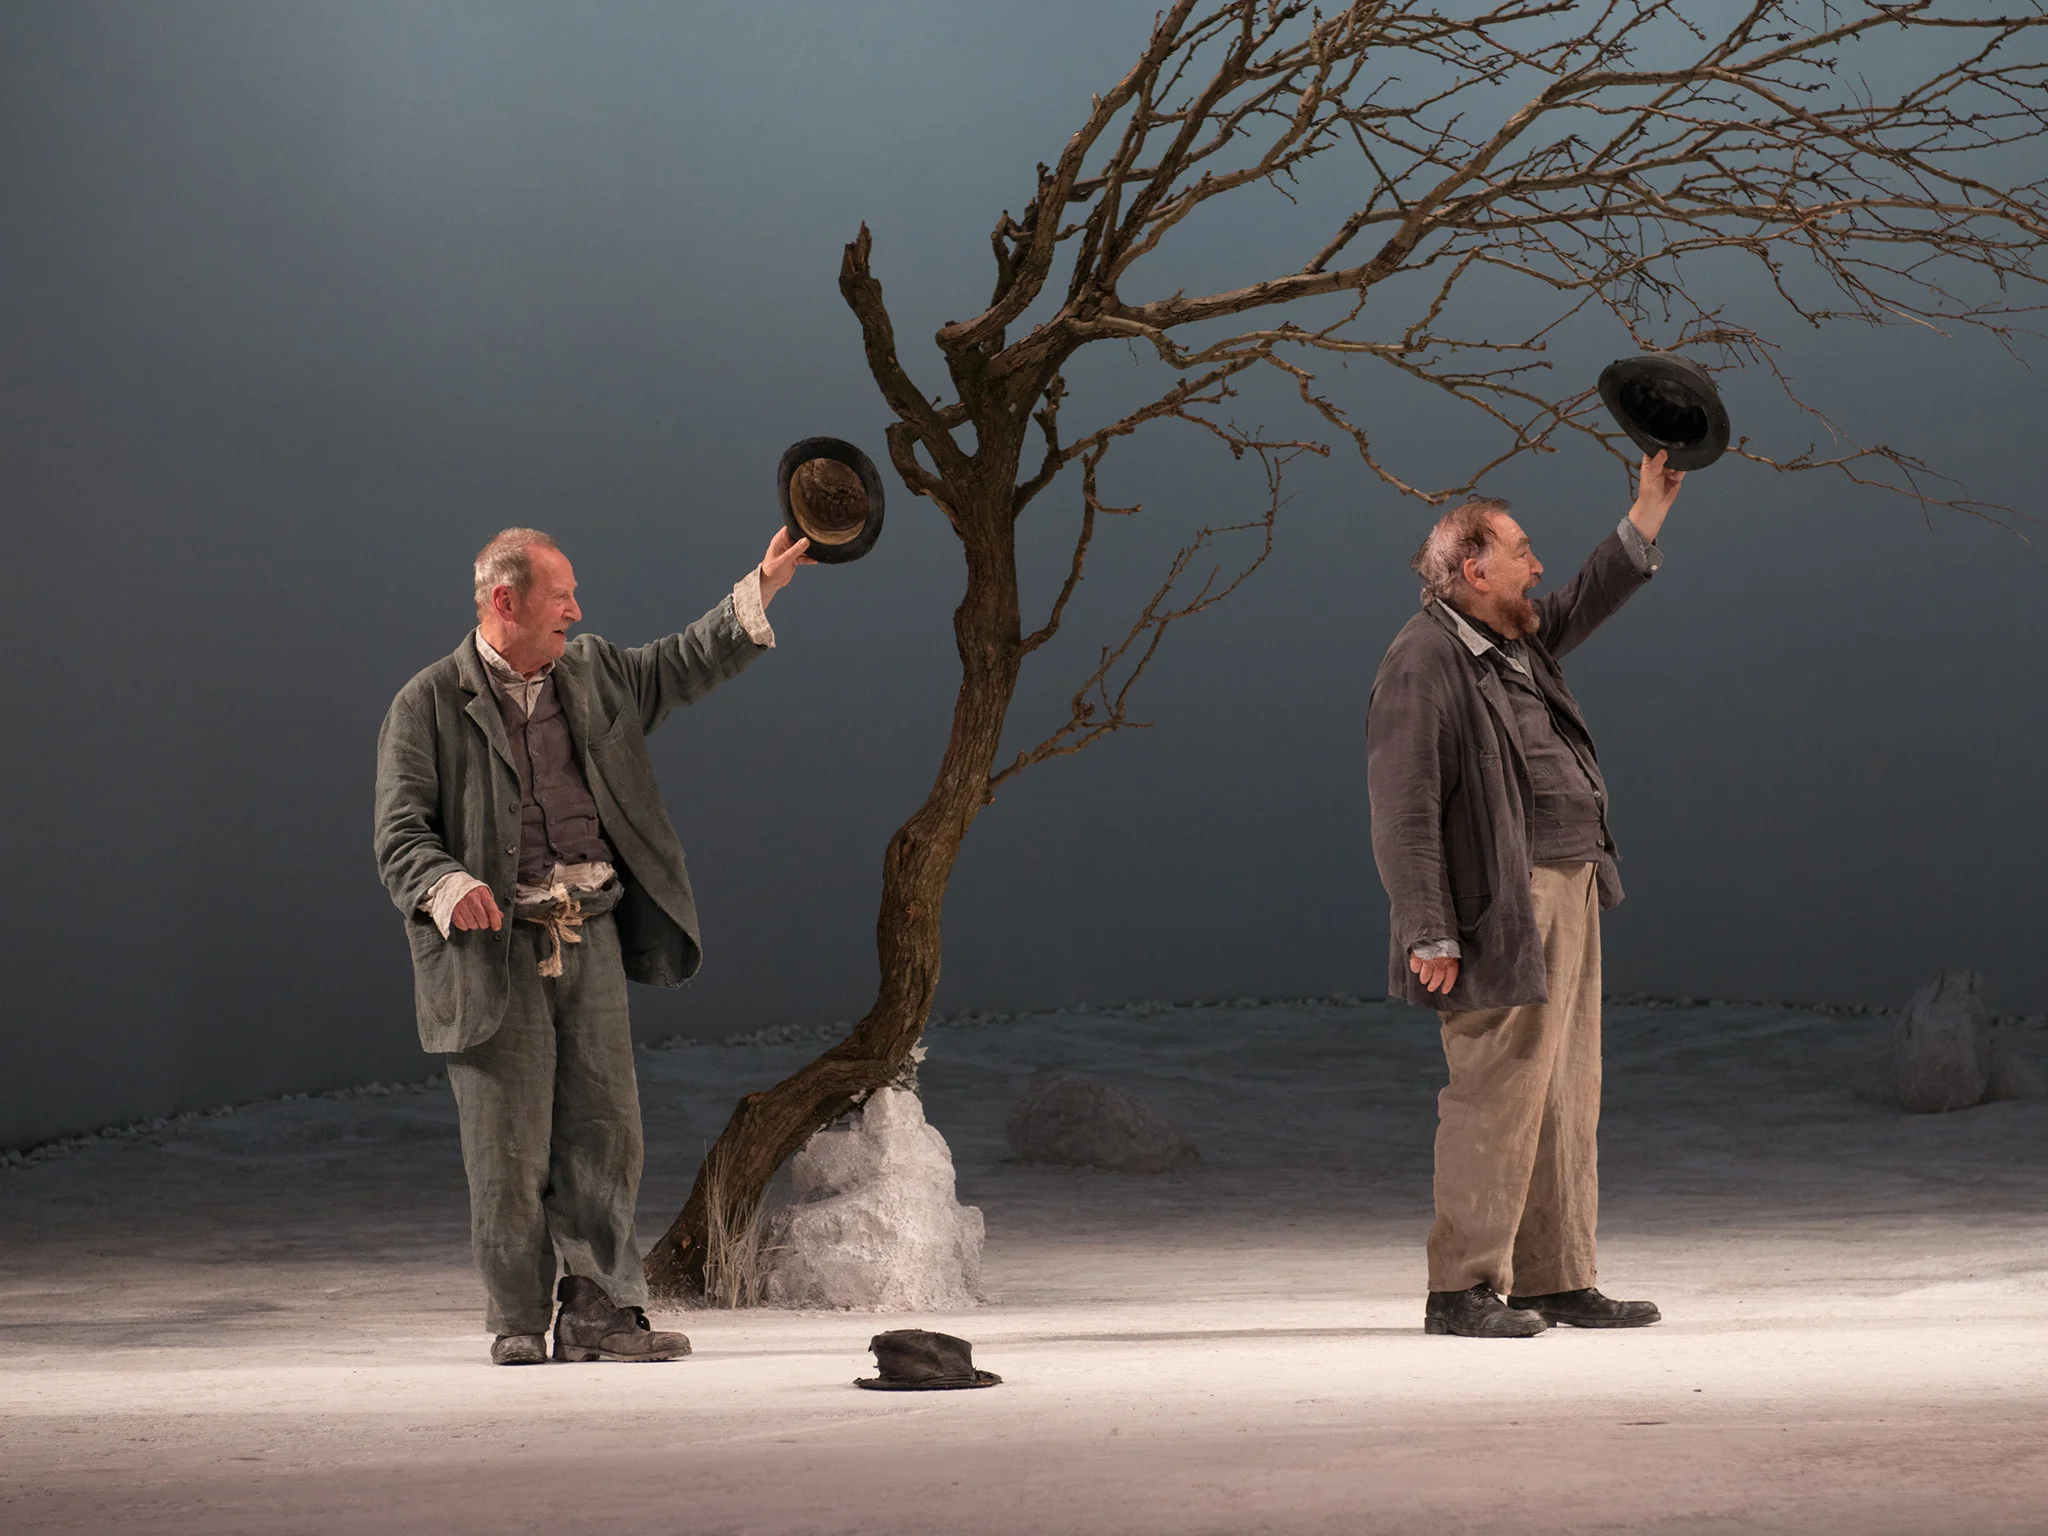
\includegraphics[width=0.95\textwidth]{godot.png}} 
\caption{Une scène du drame ``En attendant Godot"}
\end{figure}

\begin{figure}[H] 
\center{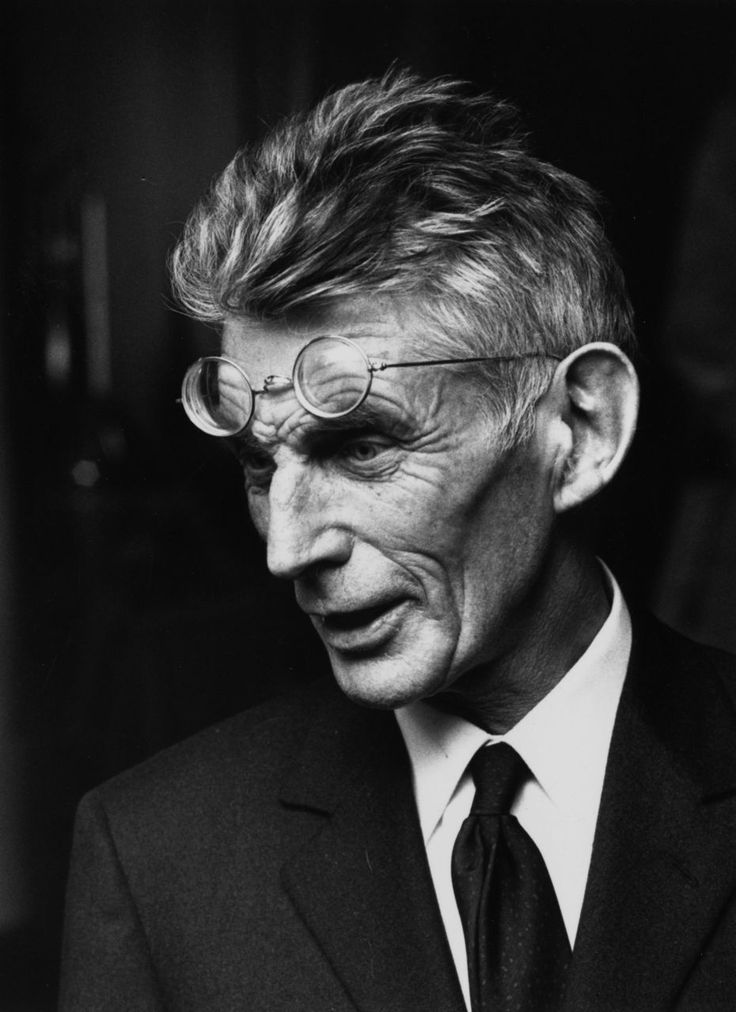
\includegraphics[width=0.4\textwidth]{beckett.jpg}} 
\caption{Le portrait de Samuel Beckett (1906-1989)}
\end{figure}
Parmi les dramaturges dans cette époque, Samuel Beckett,écrivain irlandais et figure majeure du théâtre de l'absurde, est le plus représentant. Samuel Beckett a influencé le théâtre français du 20ème siècle avec ses pièces expérimentales et minimalistes. Parmi ses œuvres les plus célèbres, on peut citer ``En attendant Godot"\mycite{beckett2006attendant}. ``En attendant Godot" est considéré comme une œuvre majeure du théâtre de l'absurde, caractérisé par l'absence de structure narrative et la réduction de l'intrigue à sa plus simple expression\mycite{harvey1960art}. Beckett a également écrit d'autres pièces emblématiques telles que ``Fin de partie", ``Oh les beaux jours" et ``Krapp's Last Tape". Ses pièces ont influencé de nombreux autres dramaturges et cinéastes, et ont inspiré de nouvelles formes de théâtre expérimental\mycite{bair1990samuel}. Beckett a également reçu de nombreux prix et distinctions pour son travail, y compris le Prix Nobel de littérature en 1969. 

\subsection{Brève Histoire du Théâtre Chinois}
Le théâtre chinois possède une histoire riche remontant à l'Antiquité, avec des racines dans les rituels et les présentations folkloriques traditionnelles. Les premières formes de théâtre chinois comprenaient des présentations de chant et de danse, ainsi que des ombres chinoises, qui ont évolué en formes plus élaborées telles que l'opéra de Pékin au XVIIIe siècle. Tout au long des siècles, le théâtre chinois a connu de nombreuses transformations et adaptations, notamment l'incorporation de l'art scénique de style occidental et de sujets modernes. Malgré des périodes de répression et de censure, le théâtre chinois continue de prospérer aujourd'hui, avec une variété de styles régionaux et de genres qui mettent en valeur l'héritage culturel unique et l'innovation artistique de la Chine.

Aujourd'hui, le théâtre chinois reste un élément important de la culture chinoise, avec une présence et une reconnaissance internationales croissantes. Des formes traditionnelles telles que l'opéra de Pékin au théâtre expérimental contemporain, le théâtre chinois continue de captiver le public avec ses présentations dynamiques et son riche héritage culturel. Dans la partie suivante, nous detaillerons les caractéristiques particulière de chaque époque.
\subsubsection{Théâtre Ancien (Avant la Dynastie Tang)}
Dans l'histoire du théâtre chinois, la période précédant la dynastie Tang peut être divisée en trois étapes : les danses rituelles antiques, la formation des pièces de théâtre avant l'époque des Royaumes combattants et la période prospère de l'époque Han\mycite{22}.

Les danses rituelles antiques étaient l'une des formes de danse les plus anciennes en Chine. Elles consistaient généralement en des mouvements tels que des sauts et des rotations, destinés à honorer les divinités ou les ancêtres. Cette forme a progressivement évolué en une forme de danse religieuse, et est devenue une composante importante des rituels pendant la dynastie Zhou.

Pendant la période précédant l'époque des Royaumes combattants, les pièces de théâtre ont progressivement pris forme comme une forme d'art indépendante en Chine. L'une des premières pièces de théâtre connues était ``Baiqi Hanxin", mentionnée dans ``Les Annales de Zuo". À cette époque, les pièces de théâtre avaient souvent pour thème des histoires historiques ou mythologiques, généralement destinées à commémorer ou célébrer un événement ou une fête importante. Les pièces de théâtre étaient également appelées ``yue" à l'époque, et les acteurs étaient généralement des membres de l'aristocratie ou des artistes professionnels.

À l'époque de la dynastie Han, le théâtre a commencé à prospérer et a été largement présenté et apprécié. Selon les annales historiques, les pièces de théâtre de l'époque comprenaient de nombreuses formes, telles que les ``grandes pièces", les ``petites pièces", les ``fu" et les ``ya yue"\mycite{13}. Les grandes pièces étaient généralement des pièces de théâtre d'histoire longues jouées par des acteurs professionnels, tandis que les petites pièces étaient des comédies ou des présentations de théâtre plus courtes organisées par des amateurs. Le fu et le ya yue étaient des formes de présentations plus élégantes, souvent destinées à des banquets ou à des divertissements.

En ce qui concerne les pièces de théâtre, de nombreux classiques sont apparus à l'époque de la dynastie Han, tels que ``Le palais d'automne de Han" et ``Le Livre des Filles". En même temps, le théâtre de l'époque Han a également été influencé par la musique, la danse et les costumes, ce qui a conduit à une plus grande diversité et sophistication dans les présentations théâtrales.

\subsubsection{Théâtre du Dynastie Tang (618-907 après JC)}
La dynastie Tang est considérée comme une période de gloire dans l'histoire du théâtre chinois. Le développement du théâtre Tang remonte aux danses et musiques de cour de l'époque de l'apogée de la dynastie Tang, qui comprenaient des pièces de musique et de danse de cour, constituant ainsi une base importante pour le développement du théâtre Tang. Le quyi, ou les arts de la scène populaires, étaient également une autre source importante du développement du théâtre Tang, se référant aux formes de représentation théâtrale principalement orales et incluant le chant, la récitation, le jeu et d'autres éléments\mycite{14}.

Les principales formes de théâtre de la dynastie Tang incluent le Tángdiào, le Tàipíngdiào, le Zuìyíndiào, le Qīngyī, le Cǎichá et le Kūnqǔ. Parmi ceux-ci, le Tángdiào est la forme de théâtre la plus représentative de la dynastie Tang, basée sur les chansons populaires, les danses et les œuvres littéraires de la dynastie Tang, combinant ainsi différentes formes d'art de la culture Tang pour offrir une grande valeur littéraire et artistique. Le Tàipíngdiào est une variante du Tángdiào qui met l'accent sur le chant rapide pour exprimer les émotions et les coutumes de la société Tang. Le Zuìyíndiào est une autre forme de théâtre représentative de la dynastie Tang, mettant l'accent sur les chansons mélodieuses et les chants rapides pour exprimer la vie et les difficultés des gens de la classe inférieure de la société Tang. Le Qīngyī est une forme de quyi représentative, mettant en scène les costumes ``Qīngyī" pour exprimer les coutumes et les traditions de la dynastie Tang. Le Cǎichá est une forme de théâtre-dansant de la dynastie Tang, qui exprime la vie laborieuse du peuple Tang à travers le thème de la cueillette du thé. Le Kūnqǔ est l'une des formes de théâtre les plus anciennes, qui a fusionné de nombreuses formes artistiques de la dynastie Tang, telles que la musique, le chant, la danse et la littérature, pour devenir une branche importante de l'histoire du théâtre chinois.
\begin{figure}[H] 
\center{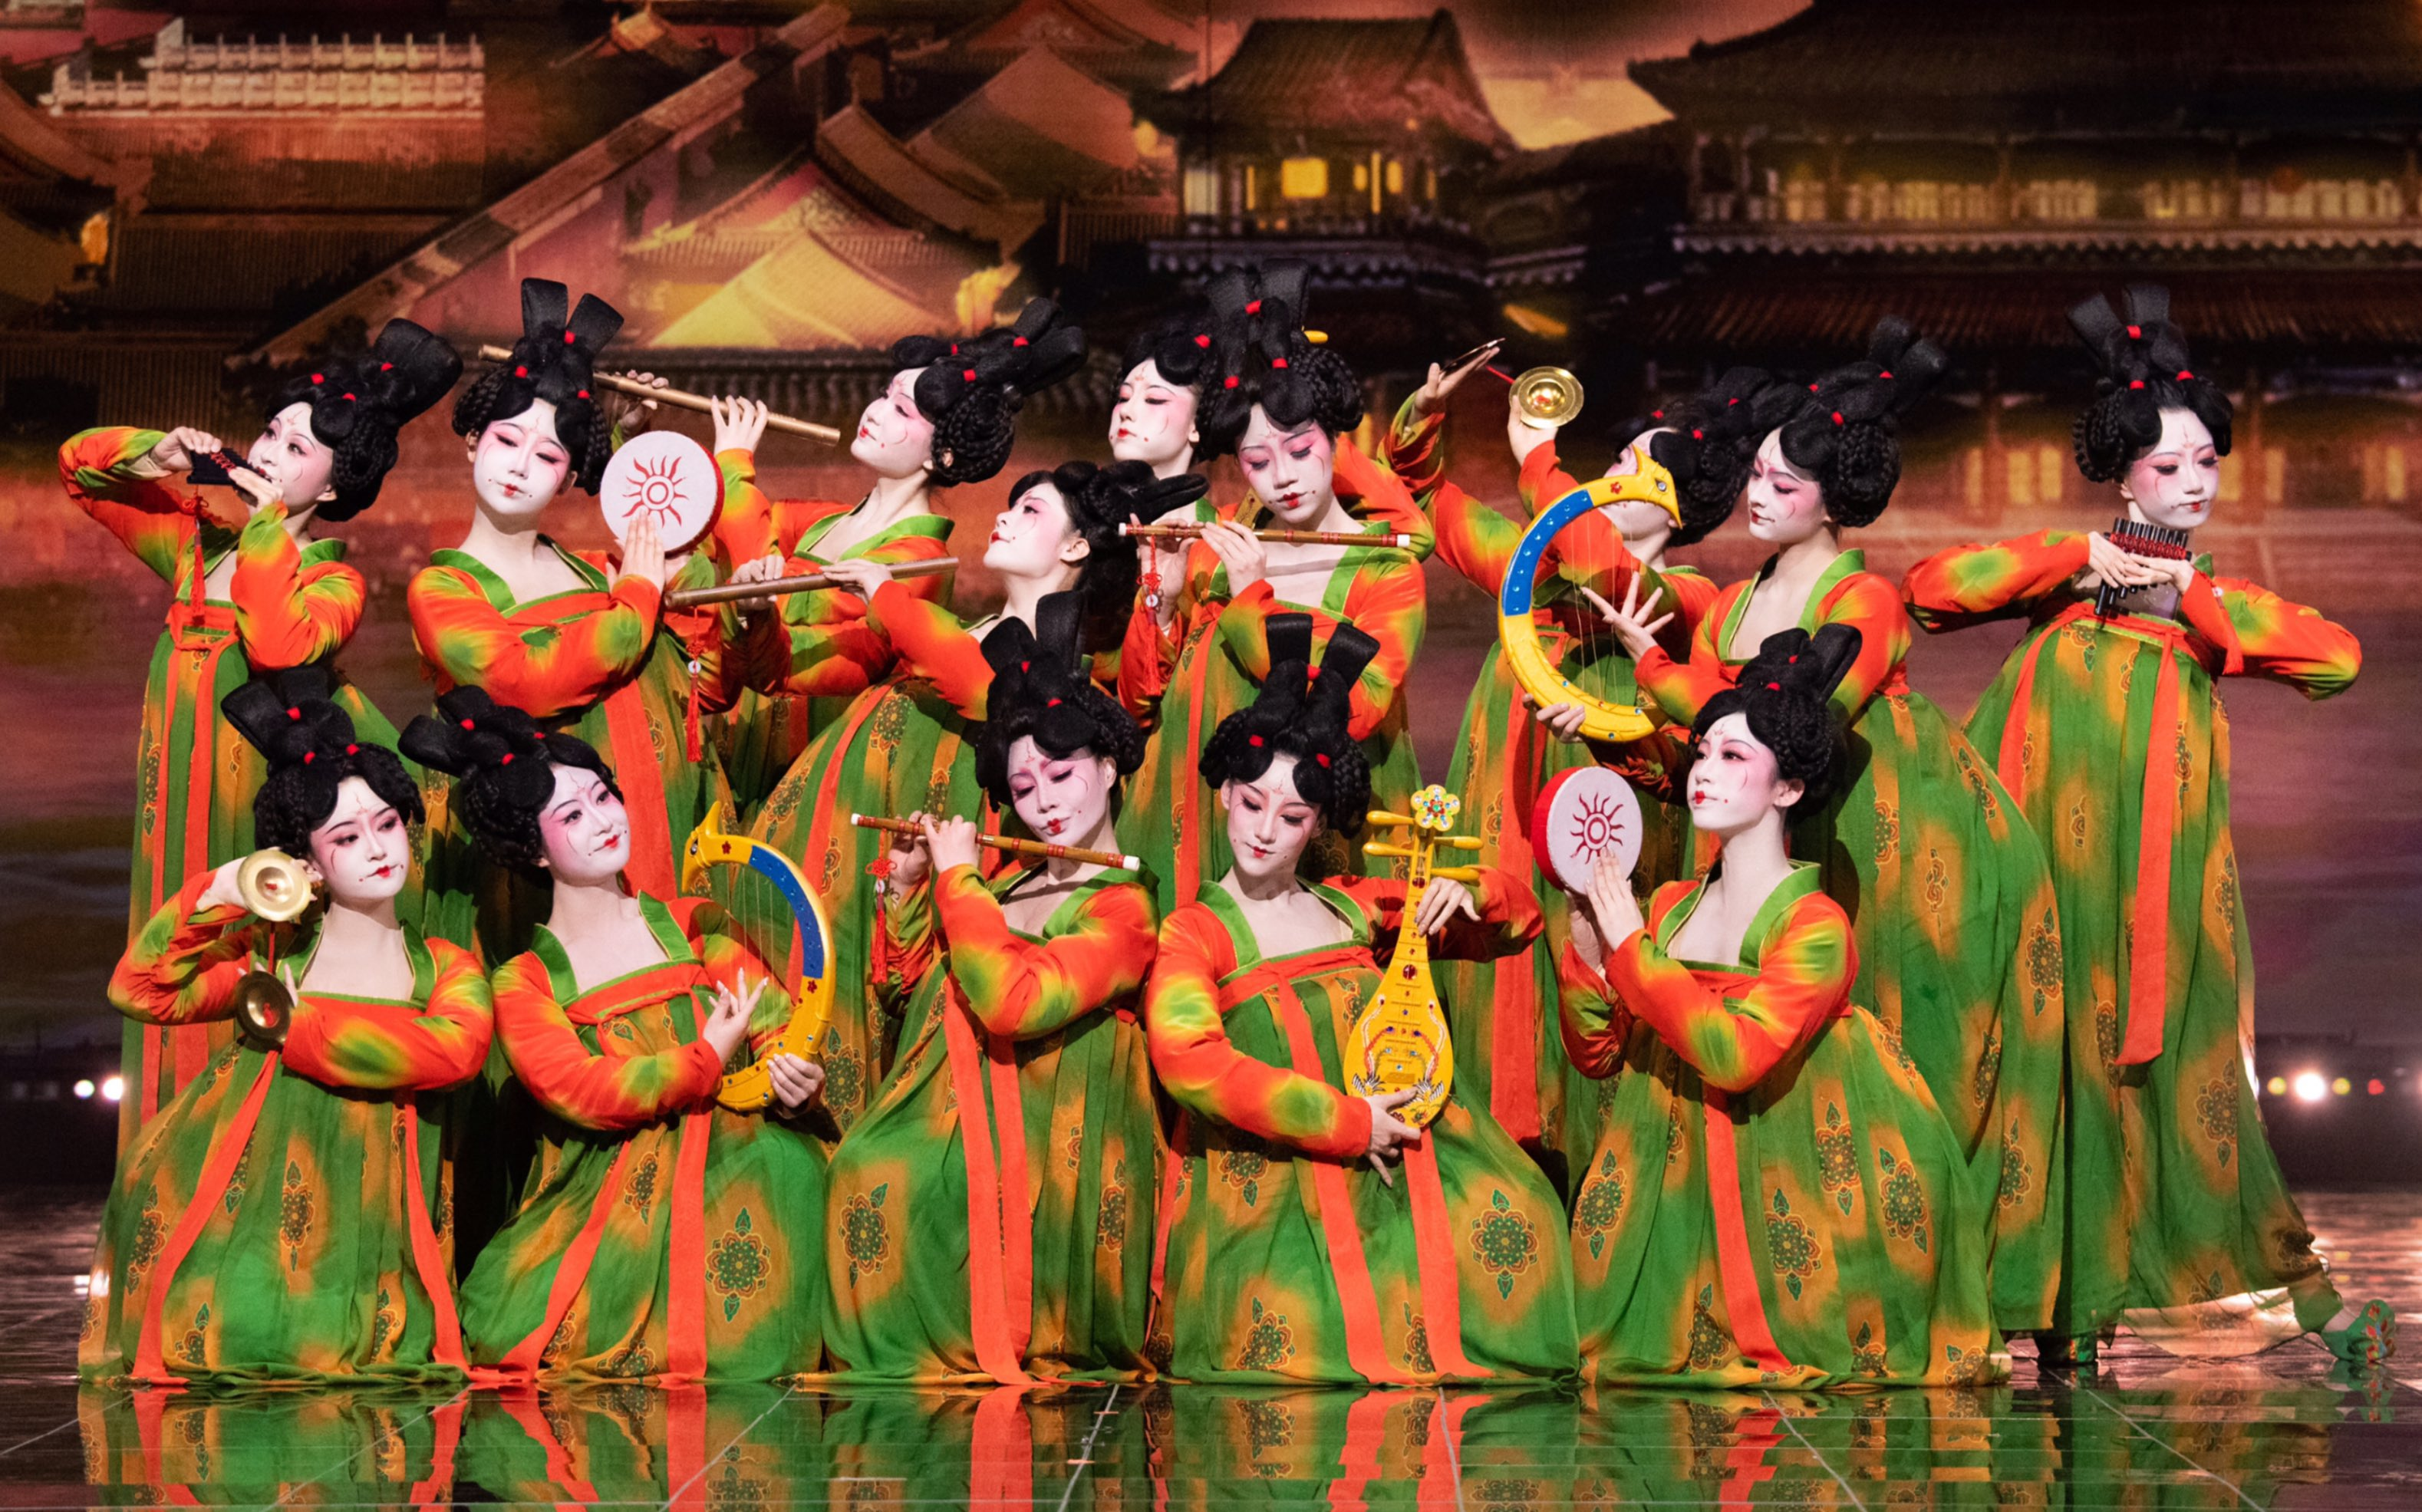
\includegraphics[width=0.95\textwidth]{tang.jpg}} 
\caption{Une scène de théâtre-dansant de la Dynastie Tang}
\end{figure}
Le théâtre Tang, tout en étant une forme d'art de représentation, a également mis l'accent sur l'expression littéraire et l'innovation, créant ainsi des œuvres littéraires ayant un style unique et un charme artistique. Le théâtre Tang a fusionné de nombreuses formes littéraires de la dynastie Tang, telles que la poésie, l'essai, la prose et la musique, parmi lesquelles se trouvent des chefs-d'œuvre artistiques à la hauteur du niveau culturel élevé de la dynastie Tang, ainsi que des œuvres littéraires populaires reflétant la vie quotidienne et les expressions courantes.

\subsubsection{Théâtre du Dynastie Yuan (1271-1368)}
La dynastie Yuan est une période importante de l'histoire du théâtre chinois, connue pour ses formes de théâtre variées et prospères. Au cours de la dynastie Yuan, le théâtre a connu un tournant historique, avec des changements radicaux dans les formes de représentation, les sujets des pièces et les styles artistiques.

Le développement du théâtre à l'époque Yuan remonte aux débuts de la Nanguan et du Beiqu, deux formes de théâtre régionales. La Nanguan était une forme de théâtre local du sud de la Chine, connue pour son intrigue serrée, ses personnages bien définis, ses airs de chant doux et mélodieux et sa musique variée. Le Beiqu, quant à lui, était une forme de théâtre de cour créée au début de la dynastie Yuan pour le palais impérial et les fonctionnaires, connue pour son style élégant, ses airs de chant complexes et sa musique magnifique, comprenant souvent des éléments tels que des chansons et des danses de la cour ainsi que des interprétations instrumentales.

Au fil du temps, le théâtre de la dynastie Yuan a connu une série de développements et de changements. Le plus important d'entre eux était le zaju, qui est une innovation majeure dans l'art dramatique de l'époque Yuan, combinant les avantages de la Nanguan et du Beiqu, et étant rempli d'éléments de réalisme. Le zaju avait une intrigue complexe et variée, une musique riche et variée, et une forme de représentation plus libre et variée. Les scénarios de zaju étaient très variés, abordant des sujets tels que l'histoire, la mythologie, les légendes, les contes populaires, etc., avec des sujets historiques, en particulier les guerres entre les dynasties Song et Yuan, étant largement utilisés. Le zaju a également largement utilisé des éléments de tradition orale tels que des blagues et des récitations, rendant l'intrigue plus vivante et intéressante\mycite{33}.

En termes de forme de représentation, le zaju de l'époque Yuan avait un niveau artistique élevé, avec la musique et la danse étant soigneusement conçues et créées, en particulier les mouvements de danse et les expressions corporelles étant très délicats et uniques. Les acteurs ont également été très exigeants en termes de compétences et d'interprétation, exprimant une forte individualité et un fort sens de l'art. Les pièces représentatives de zaju comprennent ``L'Automne dans le palais de Han", ``Le Journal de l'Ouest" et ``Le Pavillon de la vie éternelle", etc\mycite{11}.
\begin{figure}[H] 
\center{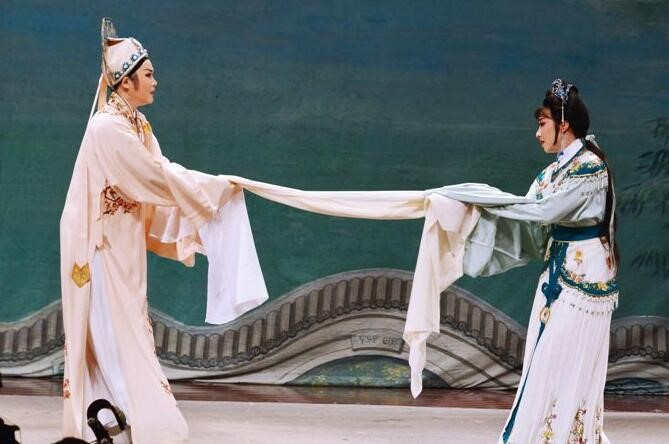
\includegraphics[width=0.95\textwidth]{zaju.jpg}} 
\caption{Une scène du zaju: ``Le Journal de l'Ouest"}
\end{figure}
Au cours du développement du théâtre de la dynastie Yuan, les artistes de théâtre ont progressivement formé leurs propres idées artistiques et styles de création, tels que les artistes Guan Hanqing, Bai Pu et Zheng Guangzu, qui ont non seulement été largement appréciés et applaudis à l'époque, mais ont également exercé une influence profonde sur le développement ultérieur de l'art dramatique. 

\subsubsection{Théâtre du Dynastie Ming \& Qing (1368-1911)}
Le théâtre du début de la dynastie Ming était encore similaire à celui de la dynastie Yuan, divisé en ``opéra du sud" et ``opéra du nord". Au milieu et à la fin de la dynastie Ming, le développement de l'opéra s'est diversifié, avec l'émergence d'une variété d'opéras locaux, tels que les opéras Huizhong, Min et Cantonais.

Le développement du théâtre chinois sous la dynastie Qing est une période très importante de l'histoire du théâtre chinois. Les tendances multiples de l'évolution du théâtre et de la musique ont conduit à la création de différentes formes de théâtre, comme l'opéra de Pékin et l'opéra de Pingju, chacune ayant ses caractéristiques propres. Cette période de développement peut être divisée en trois étapes\mycite{44}.

Au début de la période Qing, la traditionnelle forme de théâtre dominait encore, mais la diversité des formes de spectacle et des contenus de pièces de théâtre a commencé à émerger, telles que l'opéra de Pékin et l'opéra cantonais. Les pièces de théâtre de cette époque, également appelées les ``quatre grands opéras historiques", étaient principalement basées sur des sujets légendaires historiques. La musique utilisait différents instruments tels que des plaques, des erhus, des suonas, des gongs et des tambours, en mettant l'accent sur les présentation de la gestuelle, du chant et des masques. En même temps, les différentes formes de théâtre locaux ont également été largement développées, tels que l'opéra de Pingju, l'opéra cantonais, l'opéra du Fujian, etc., chacun ayant ses propres caractéristiques dans la forme de représentation, l'accompagnement musical et les personnages.

Au milieu de la période Qing, les formes de spectacle et les contenus des pièces de théâtre se sont encore enrichis, le nombre de pièces de théâtre a progressivement augmenté, et les thèmes étaient plus variés. À cette époque, l'opéra de Pingju est devenu l'un des principaux genres de théâtre chinois, caractérisé par une intrigue serrée et une description émotionnelle délicate, en tant que forme artistique pour représenter la vie quotidienne et la réalité sociale. En même temps, l'opéra de Pékin a également continué à progresser dans les techniques de présentation, les sujets de pièces de théâtre, etc., formant plusieurs écoles de théâtre telles que les ``deux huang" et les ``deux xiao".

À la fin de la période Qing, les formes de spectacle et les contenus de pièces de théâtre ont continué à innover, et les différentes formes de théâtre ont commencé à se mélanger et à s'inspirer mutuellement. À cette époque, l'opéra de Pékin était déjà devenu l'un des genres de théâtre les plus représentatifs de la Chine, avec un style et des techniques relativement matures. En même temps, des genres tels que l'opéra de Pingju et l'opéra de Kunqu ont également connu un grand développement dans les techniques instrumentales et lyriques, ainsi que la mise en scène, etc.
\begin{figure}[H] 
\center{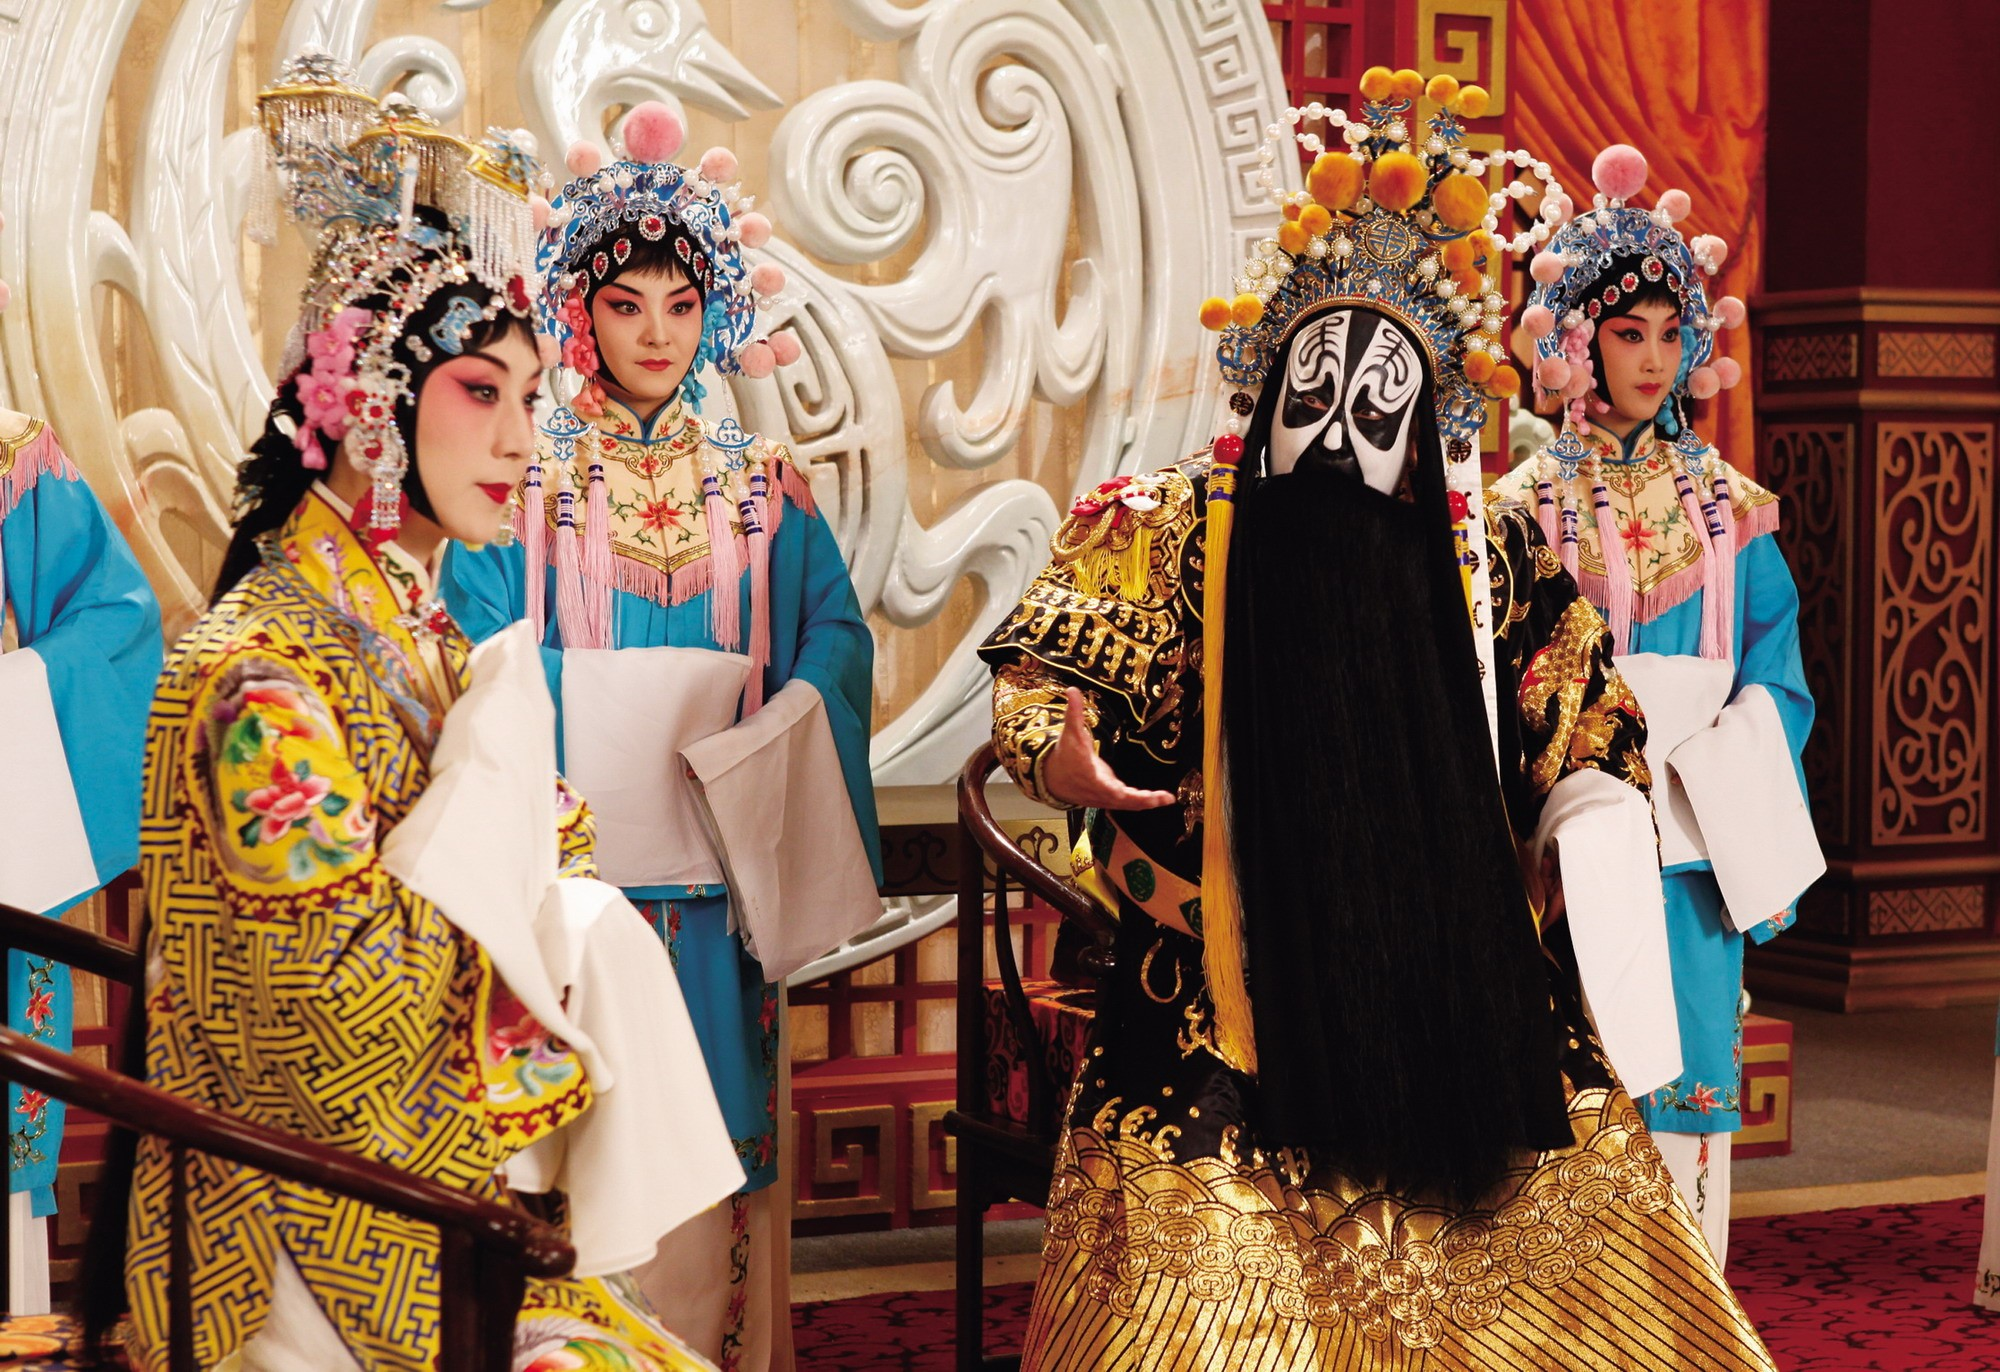
\includegraphics[width=0.95\textwidth]{jingju.jpg}} 
\caption{Une scène de L'opéra de Pékin: ``Adieu ma concubine"}
\end{figure}
L'opéra de Pékin se caractérise par une combinaison unique de chant, de danse, de jeu d'acteur et d'acrobaties, accompagnée d'instruments de musique traditionnels chinois. Les représentations comportent des costumes et un maquillage élaborés, les interprètes utilisant des mouvements et expressions faciales exagérés pour transmettre des émotions et raconter des histoires. Les histoires sont souvent inspirées de l'histoire, de la mythologie et de la littérature chinoises, et sont interprétées de manière stylisée qui met l'accent sur la symbolique et la métaphore.

\subsubsection{Théâtre de l'Ere Moderne}
Après la chute de la dynastie Qing en 1911, le théâtre chinois a subi de grands changements et des a dû faire preuve de s'adapter aux influences étrangères. Avec l'établissement de la République de Chine, les formes traditionnelles de théâtre chinois ont été progressivement remplacées par des formes occidentales de théâtre et de drame, entraînant le déclin de nombreux styles et genres régionaux. Le Mouvement du 4 mai en 1919 a suscité un intérêt renouvelé pour la culture et le nationalisme chinois, conduisant à l'émergence d'une nouvelle vague de théâtre qui cherchait à combiner les techniques occidentales avec des thèmes et motifs chinois. Ce mouvement était illustré par les œuvres de dramaturges tels que Cao Yu, Tian Han et Guo Moruo, qui ont exploré des thèmes de justice sociale, de révolution et d'identité nationale.

L'établissement de la République populaire de Chine en 1949 a entraîné d'autres changements dans le théâtre chinois, le gouvernement promouvant le théâtre révolutionnaire qui cherchait à éduquer et inspirer les masses. Cela a conduit à l'émergence de ``pièces modèles" telles que ``La fille aux cheveux blancs" et ``L'armée des femmes rouges", qui sont devenues extrêmement populaires pendant la Révolution culturelle. Cependant, cette période a également vu la suppression et la censure de nombreuses formes traditionnelles de théâtre chinois, conduisant au déclin des styles régionaux et à la perte de nombreuses traditions culturelles.

\begin{figure}[H] 
\center{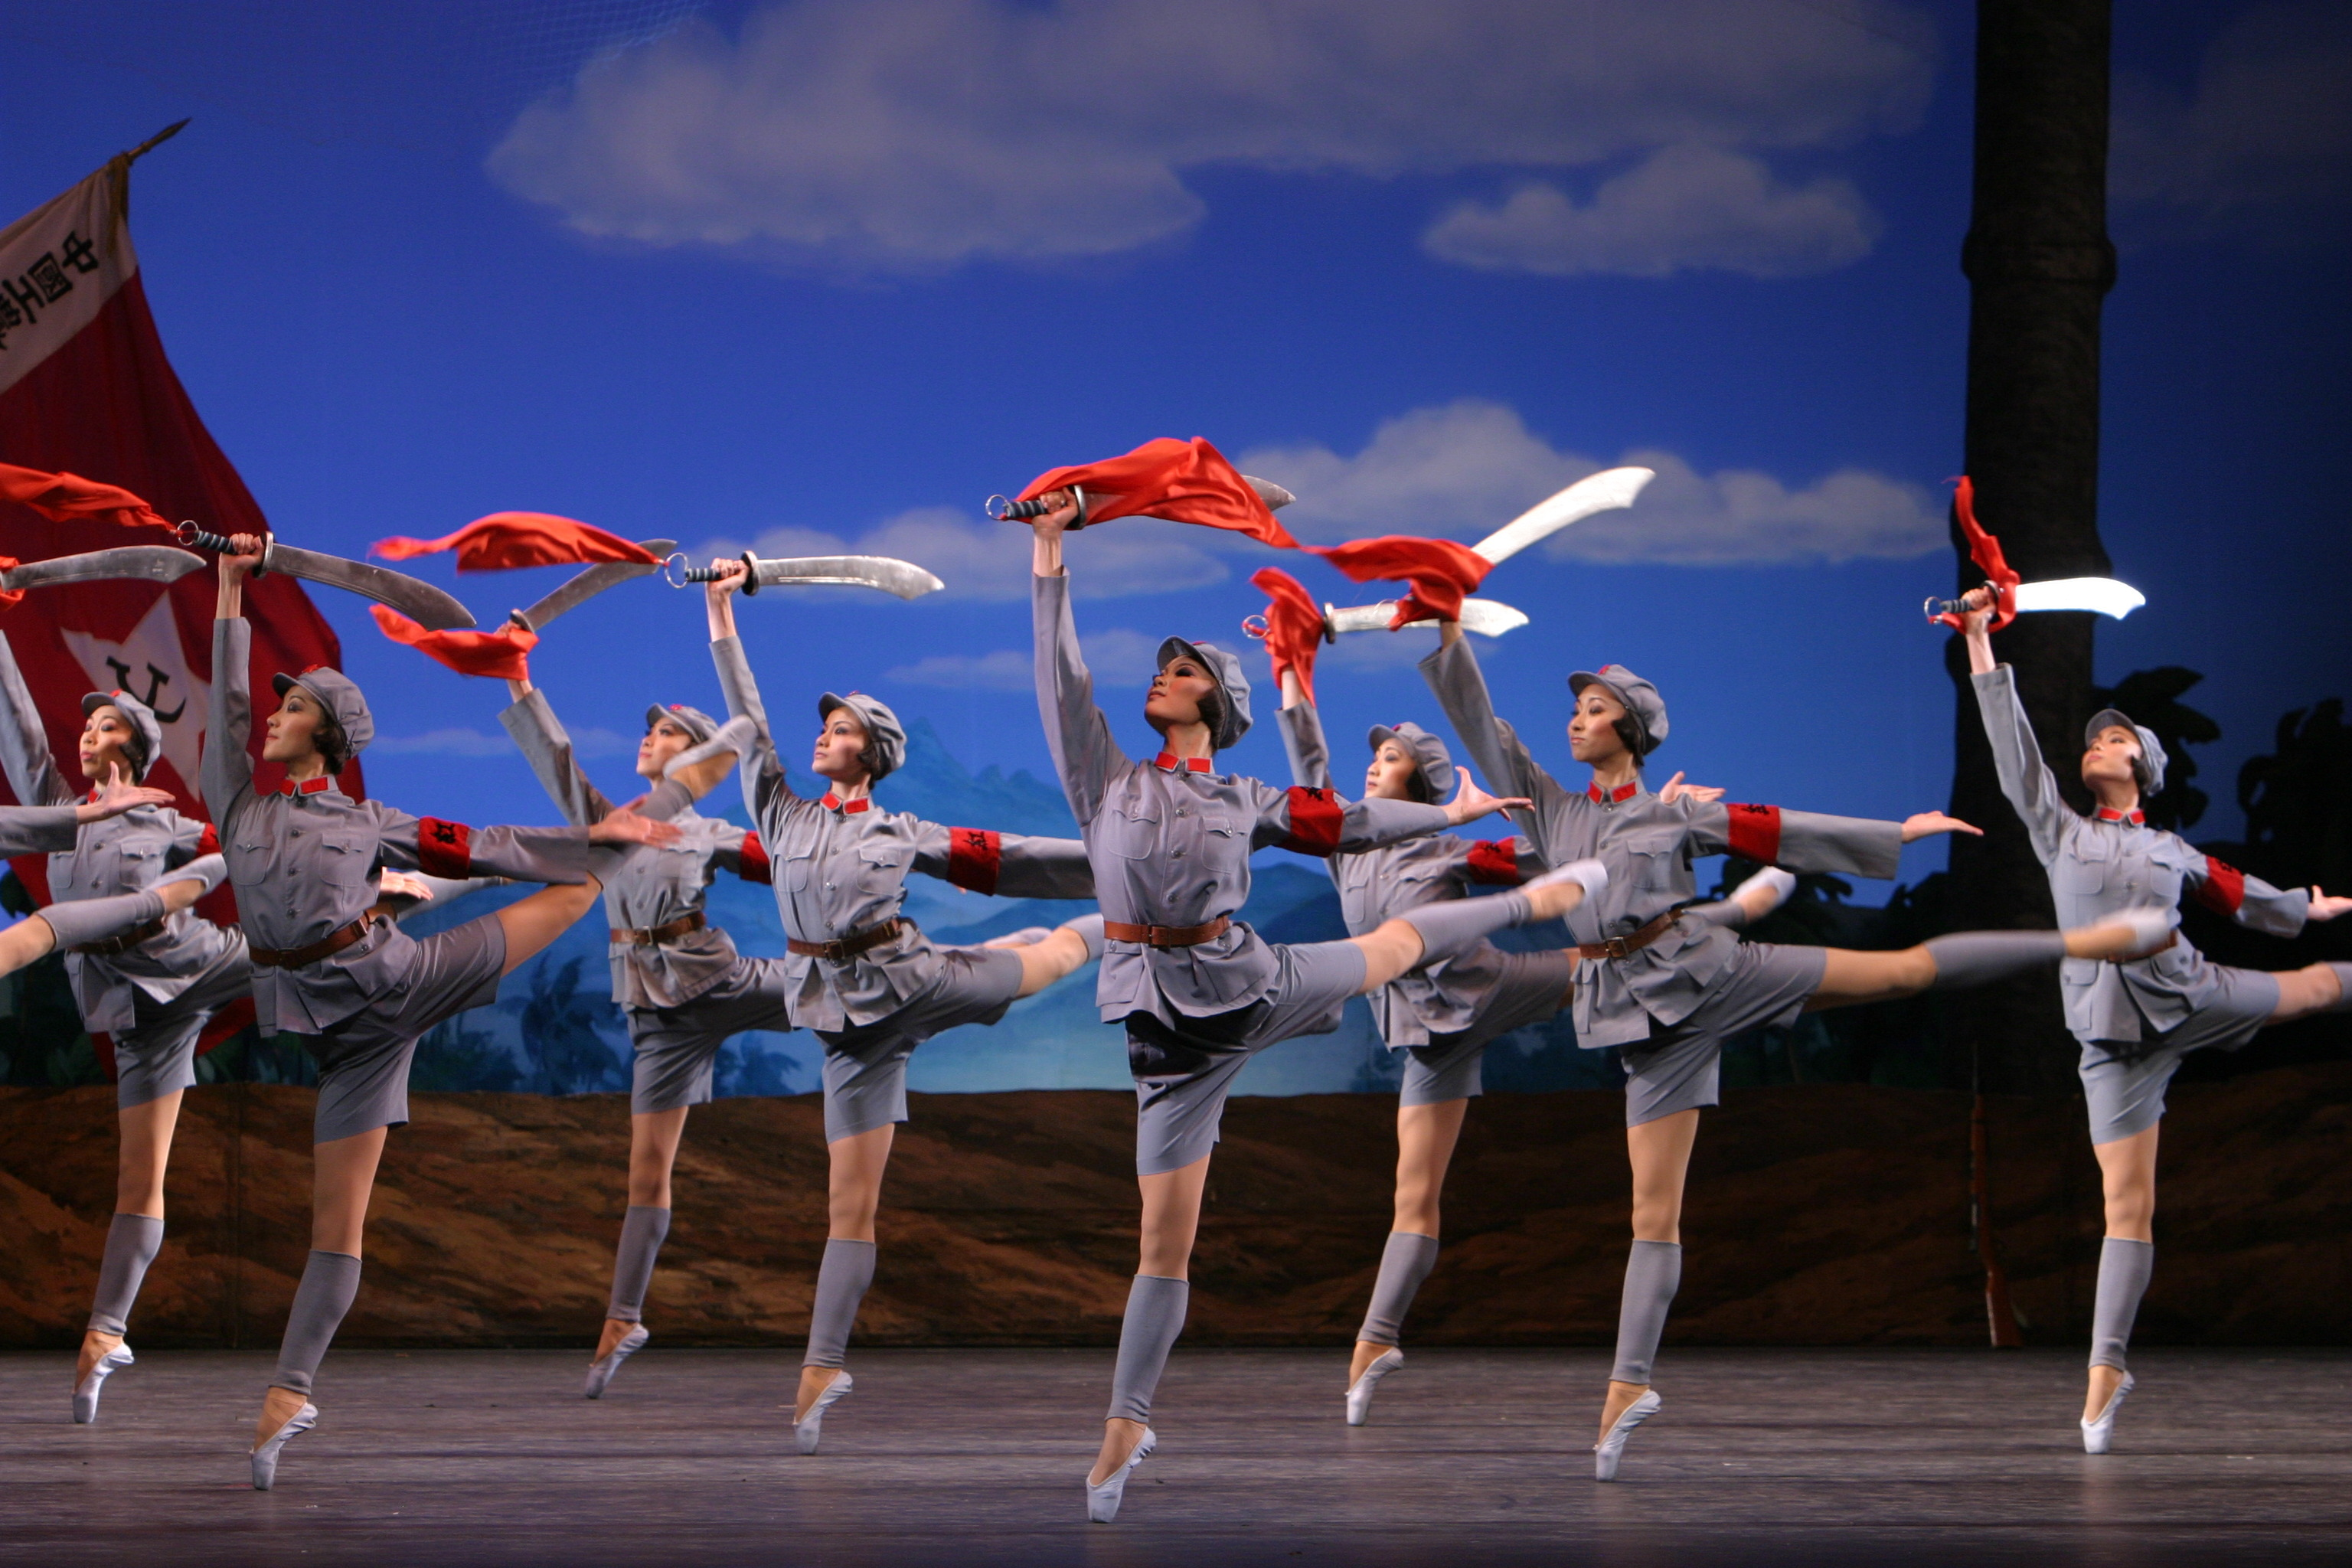
\includegraphics[width=0.9\textwidth]{hongse.jpg}} 
\captionsetup{justification=centering, singlelinecheck=false}
\caption{Une scène du théâtre moderne: ``L'armée des femmes rouges". On pourrait voir clairement la caractérisation des costumes et du maquillage.}
\end{figure}

Dans les années 1980s et 1990s, le théâtre chinois a connu une résurgence, avec un intérêt renouvelé pour les formes traditionnelles telles que l'opéra de Pékin et l'opéra kunqu, ainsi qu'un intérêt croissant pour le théâtre expérimental et d'avant-garde. Cette période a vu l'émergence de nouveaux dramaturges, metteurs en scène et interprètes qui ont repoussé les limites du théâtre chinois et exploré de nouveaux thèmes et techniques. Aujourd'hui, le théâtre chinois continue d'évoluer et de s'adapter aux changements sociaux et culturels, avec une variété de styles et de genres qui mettent en valeur le riche patrimoine culturel et l'innovation artistique de la Chine.

%\begin{enumerate}
%\item Théâtre ancien (avant la dynastie Tang) : Cette période comprend les premières formes de théâtre chinois, telles que le "Song of Chu" et le "Zaju" (pièces de variétés). Ces pièces étaient jouées dans des théâtres en plein air et mettaient en scène de la musique, de la danse et des acrobaties. 
%\item Dynastie Tang (618-907) : Au cours de cette période, le théâtre chinois devient plus sophistiqué et commence à intégrer des éléments de poésie et de littérature. C'est à cette époque qu'apparaît le style d'opéra "Kunqu", qui est encore joué aujourd'hui. 
%\item Dynastie Yuan (1271-1368) : La dynastie Yuan voit l'essor du style théâtral "Zaju", qui combine le chant, la danse et le jeu d'acteur. Cette période voit également l'émergence des genres "Chuanqi" (contes merveilleux) et "Zaju" (pièces de variétés).
%\item La dynastie Ming (1368-1644) : La dynastie Ming est un âge d'or pour le théâtre chinois, avec le développement du style "Jingju" (opéra de Pékin). Ce style combine le chant, la danse et l'acrobatie, et se caractérise par des costumes et des maquillages élaborés.
%\item Dynastie Qing (1644-1912) : Sous la dynastie Qing, le théâtre chinois continue d'évoluer, avec l'émergence de nouveaux styles tels que le "Huaju" (théâtre parlé) et le "Yueju" (opéra cantonais). C'est également à cette époque que les influences occidentales ont commencé à être intégrées dans le théâtre chinois. 
%\item L'ère moderne (1912-aujourd'hui) : À l'ère moderne, le théâtre chinois a continué à évoluer et à s'adapter aux changements. De nouveaux styles et genres sont apparus, tels que le style "Xiqu" (opéra chinois) et le style "Dianying" (film chinois).
%\end{enumerate}

%\subsection{Bilan du Chapitre}
%....

\newpage
\fancyhead[LH]{上海交通大学学位论文}
\fancyhead[RH]{Chapitre II\quad Différences et Similitudes des Théâtres} \label{sec:2}
\section{Différences et Similitudes entre Le Théâtre Français et Chinois} \label{sec:role}
\hspace{8mm}
En tant que deux types et systèmes différents, la littérature dramatique chinoise et française présente à la fois une ``différence" relative et une ``homogénéité" relative. Cette "différence" et "homogénéité" ne se reflètent pas seulement dans la catégorie du sujet et du thème, mais également dans tous les aspects tels que l'image du personnage, la structure de l'intrigue et la technique créative. Bien que les deux échangent et communiquent rarement, il peut toujours y avoir de nombreuses similitudes frappantes. Dans ce chapitre, nous nous concentrerons sur les similitudes et les différences entre le théâtre chinois et français.

\subsection{Différences entre Le Théâtre Français et Chinois}
Le théâtre français et chinois ont beaucoup de  différences, notamment dans leur style, leur structure et leurs thèmes. On liste quelques points dessous.
\subsubsection*{1. Styles de Jeu}
Le théâtre français est souvent plus réaliste et naturaliste, cherchant à représenter la vie quotidienne et les comportements humains de manière précise et crédible. Les acteurs français ont tendance à se concentrer sur les aspects psychologiques et émotionnels de leurs personnages, et à utiliser un langage clair et direct. Le théâtre français est souvent considéré comme plus sérieux et intellectuel, avec une attention particulière accordée aux dialogues, aux personnages et à la psychologie\mycite{99}.

En revanche, le théâtre chinois est souvent plus stylisé et symbolique. Les acteurs chinois utilisent des gestes et des mouvements symboliques pour représenter des idées abstraites et des émotions, et ils peuvent également incorporer des techniques d'acrobatie, de danse et de chant dans leurs présentations. Les costumes et le maquillage sont également souvent très élaborés et symboliques, contribuant à la représentation de personnages mythiques et de divinités. Le théâtre chinois est souvent considéré comme plus visuel et spectaculaire, avec une attention particulière accordée aux mouvements et aux techniques de représentation.
\subsubsection*{2. Structure}
Le théâtre français utilise souvent une structure en actes et en scènes, avec des dialogues développés et des transitions clairement définies. Les pièces de théâtre françaises ont généralement une intrigue linéaire, où les événements se déroulent dans un ordre chronologique et logique. Les personnages et les relations entre eux sont souvent développés de manière approfondie, et les pièces ont souvent une fin claire et résolutive.

Par exemple, le drame ``Tartuffe" suit une structure linéaire classique, qui suit la règle des trois unités \footnote{Cette règle stipule que l'action d'une pièce de théâtre doit se dérouler en un seul lieu, sur une période de temps limitée et avec une unité d'action.}. La pièce suit la séquence classique de l'exposition, de l'élément déclencheur, du développement, du point culminant et de la résolution. L'exposition établit les personnages, les relations et les enjeux de la pièce, tandis que l'élément déclencheur est l'arrivée de Tartuffe, un faux dévot qui est rapidement accepté dans la famille d'Orgon, le personnage principal\mycite{cardullo2009moliere}. Le développement suit les manigances de Tartuffe pour séduire la femme d'Orgon et prendre le contrôle de la famille. Le point culminant est atteint lorsque Tartuffe menace de faire arrêter Orgon pour une affaire de droit et la résolution intervient lorsque Tartuffe est finalement démasqué et la famille est sauvée grâce à l'intervention de la justice\mycite{lancaster1929history}.
Un autre exemple, la structure du drame ``Les Misérables" de Victor Hugo peut aussi être considérée comme une structure en cinq actes(un variant de la structure linéaire, souvent utilisé dans les tragédies classiques).

Le théâtre chinois utilise souvent une structure en cycles ou multilignes. Les transitions entre les scènes sont souvent fluides et sans interruption, créant une atmosphère de continuité et de fluidité. Les personnages et les événements sont souvent représentés de manière symbolique, et l'intrigue peut comporter plusieurs niveaux de signification. Les pièces de théâtre chinoises peuvent également incorporer des chants, des danses et des acrobaties pour renforcer l'atmosphère poétique et visuelle de la représentation.

\subsubsection*{3. Caractérisation du Rôle}
La création littéraire chinoise ancienne a principalement hérité de la pensée confucéenne traditionnelle, mettant l'accent sur la fonction éducative et la valeur sociale de la littérature et de l'art. Lorsque les écrivains créent des personnages, ils se concentrent toujours d'abord sur les aspects sociaux des personnages et semblent minimiser ou même ignorer les personnalités des personnages. Les dramaturges français ont hérité de l'excellente tradition du réalisme dans la littérature humaniste, qui se concentre sur la vie et valorise l'individualité. Par conséquent, sa création dramatique peut prêter attention aux contradictions et aux conflits basés sur les pierres angulaires des personnages individuels de différents personnages, et s'efforcer de creuser et d'exprimer les caractéristiques de personnalité distinctives et proéminentes des personnages, ainsi que leur richesse émotionnelle intérieure complexe. 
La pièce de théâtre chinoise ``L'Esclave de l'argent"\mycite{78} de l'auteur de l'époque Yuan Zheng Tingyu, et la comédie ``L'Avare"\mycite{bernard1906avare} du dramaturge classique français Molière, sont toutes deux connues pour leur représentation du personnage avare. Les deux protagonistes de la pièce, Jia Ren et Harpagon, sont déjà considérés comme représentatifs de ``l'avare de l'Est" et de ``l'avare de l'Ouest". On les prend comme exemple parafait pour illustrer l'idée de l'avarie. 

\begin{figure}[H] 
\center{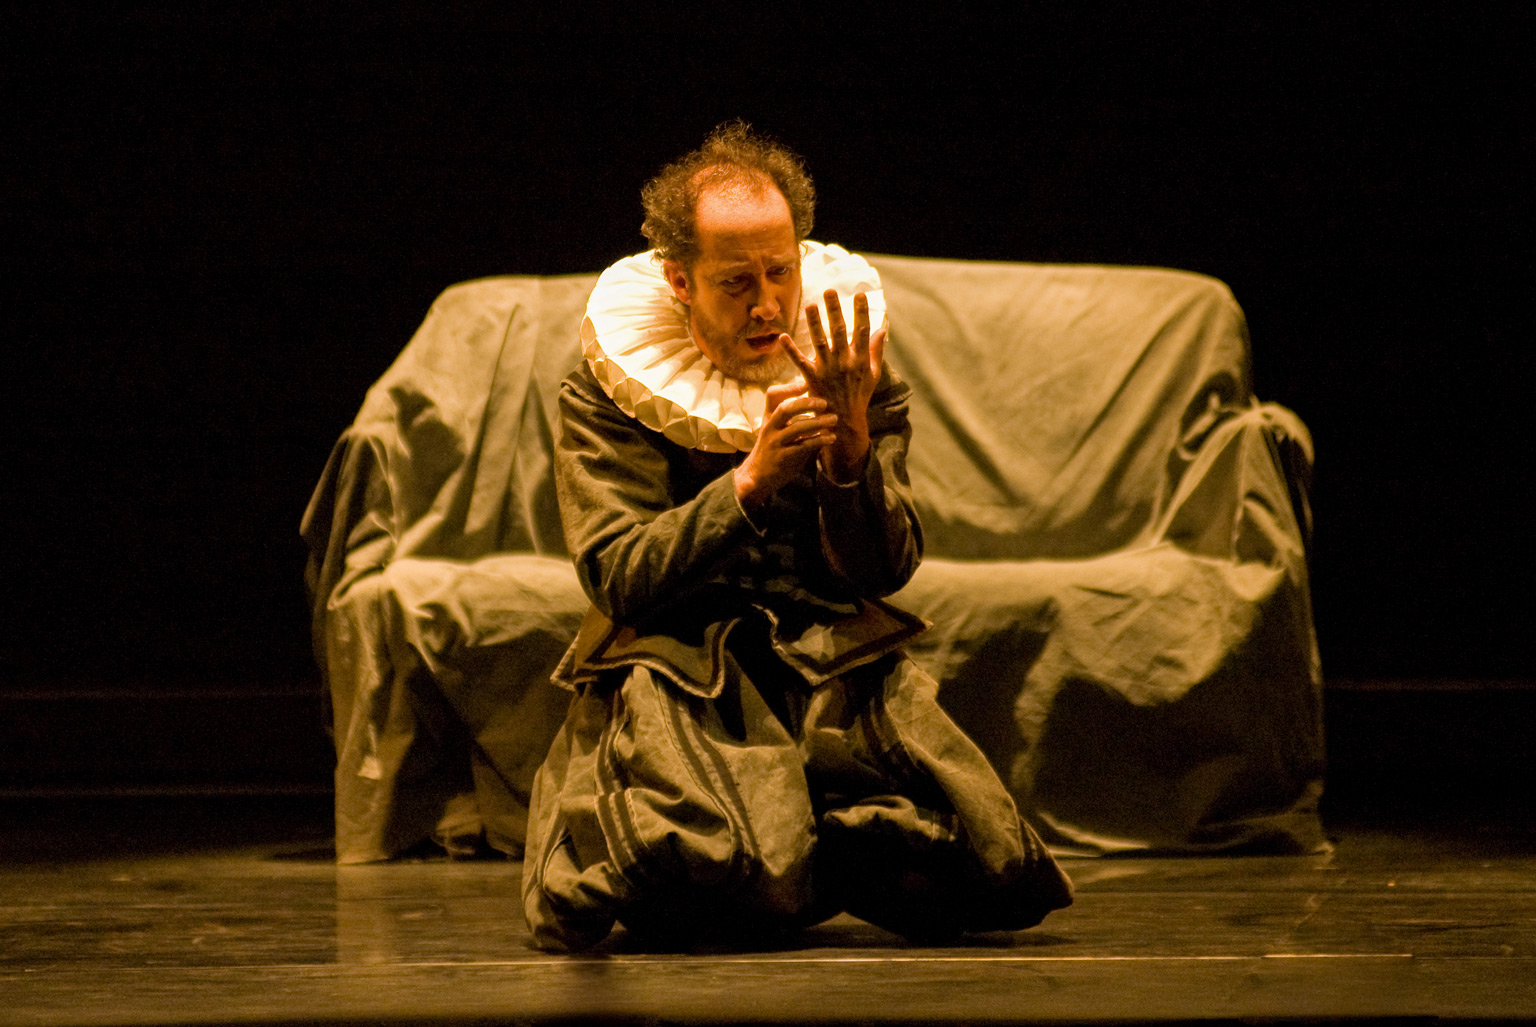
\includegraphics[width=0.9\textwidth]{avare2.jpg}} 
\captionsetup{justification=centering, singlelinecheck=false}
\caption{ ``L'Avare" de Molière: rôle de Harpagon (l'avare de l'Ouest)}
\end{figure}

\begin{figure}[H] 
\center{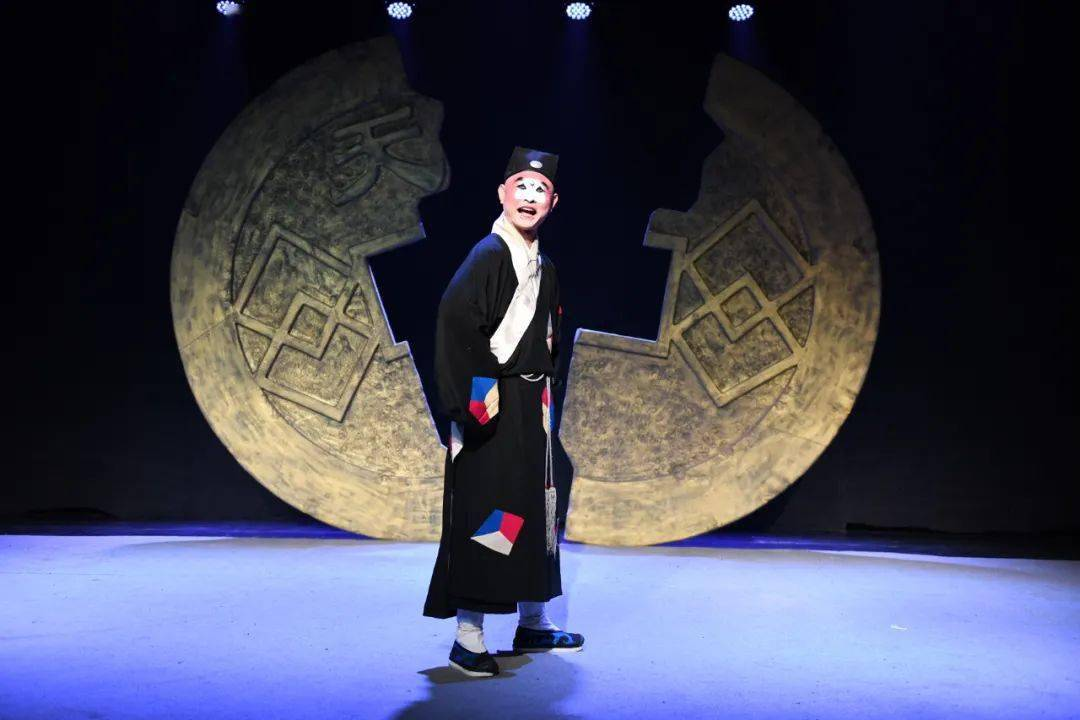
\includegraphics[width=0.9\textwidth]{kanqian.jpeg}} 
\captionsetup{justification=centering, singlelinecheck=false}
\caption{ ``L'Esclave de l'argent" de Zheng Tingyu: rôle de Jia Ren (l'avare de l'Est)}
\end{figure}

Dans ``L'Avare", Molière est doué pour faire apparaître plus de personnages sur scène, de sorte qu'ils tissent un réseau complexe de relations interpersonnelles avec les personnages principaux, et toutes sortes de conflits et d'enchevêtrements surgissent\mycite{66}. Le double conflit d'argent et d'amour entre Harpagon et Cléante père et fils; la relation compliquée entre Elise, Valère et Lord Anselme semblable au ``triangle amoureux"; Valère et Mariana et la relation de sang entre Lord Anselme et ainsi de suite; les personnages principaux sont piégés dans diverses contradictions et conflits , et leurs caractéristiques de personnalité sont affichées sous plusieurs aspects. Dans ``L'Escalve de l'argent", le dramaturge arrange essentiellement Jia Ren pour chanter un one-man show, c'est-à-dire pour atteindre l'objectif de dépeindre le personnage du personnage à travers sa propre expérience et son autodérision. Seulement dans le but de continuer l'intrigue et d'expliquer la cause et l'effet des activités du protagoniste, seuls quelques personnages secondaires sont ajoutés, et ils manquent évidemment de personnalité. Cette méthode d'écriture est déduite dans une large mesure en raison des limites de la structure et du système du zaju des Yuan - généralement un coin et quatre plis \footnote{La structure du zaju de Yuan suit cette forme canonique ``1 coin et 4 plis", Le coin pour le préambule; Les 4 plis pour 4 coupures : commencement, développement, tournure et résolution.}, et les personnages du drame expriment principalement leurs actions extérieures et leurs états psychologiques en chantant, récitant et il est peu pratique et difficile de mettre en place des personnages plus compliqués et de construire une série d'intrigues et de scènes colorées.

En termes de description des points communs et de l'individualité des personnages, ``L'Avare" et ``L'Esclave de l'argent" montrent des différences évidentes : ``L'Esclave de l'argent" se concentre sur l'expression des points communs - le personnage de ``l'avare" Jia Ren est plus mitigé. est inclus est l'élément commun, c'est-à-dire qu'il est principalement un résumé concentré des caractéristiques essentielles de toutes les sortes de seigneurs féodaux à cette époque. Apagon dans ``L'Avare" est connu pour sa description de personnalité distinctive et unique - Apagon n'est pas un avare occidental typique qui est gourmand et aime l'argent, mais un ``celui-ci" avec ses propres caractéristiques.

\subsubsection*{4. Costumes et Maquillage}
Il est facile de voir les différences de costumes et de maquillage entre le théâtre chinois et français sur scène. Nous en listons quelques-uns dans la suite.

\noindent{\textbf{Costumes:}}

$\bullet$ Le théâtre français utilise souvent des costumes qui reflètent la mode et les tendances de l'époque représentée dans la pièce, tandis que le théâtre chinois utilise des costumes traditionnels qui sont souvent très colorés et ornés de broderies complexes.

$\bullet$ Les costumes du théâtre français sont souvent conçus pour être facilement retirés ou ajustés pendant la pièce, et les costumes du théâtre chinois sont souvent très lourds et difficiles à enlever.

$\bullet$ Le théâtre français utilise souvent des costumes réalistes, mais le théâtre chinois utilise des costumes stylisés qui peuvent inclure des éléments fantastiques tels que des ailes, des queues et des cornes.

\noindent{\textbf{Maquillage}}:

$\bullet$ Le maquillage du théâtre français est généralement conçu pour accentuer les expressions faciales et les traits des acteurs, tandis que le maquillage du théâtre chinois est souvent plus symbolique et utilise des couleurs spécifiques pour représenter des personnages ou des émotions particulières.

$\bullet$ Le maquillage du théâtre français est souvent subtil et réaliste, mais le maquillage du théâtre chinois peut être très dramatique et stylisé, avec des lignes épaisses et des couleurs vives.

$\bullet$ Les acteurs de théâtre français ne portent souvent pas de masques, par contre le théâtre chinois utilise souvent des masques pour représenter certains personnages ou émotions.

%\begin{figure}[H]
%\centering
%\begin{minipage}{0.47\textwidth}
%
%    \centering
%    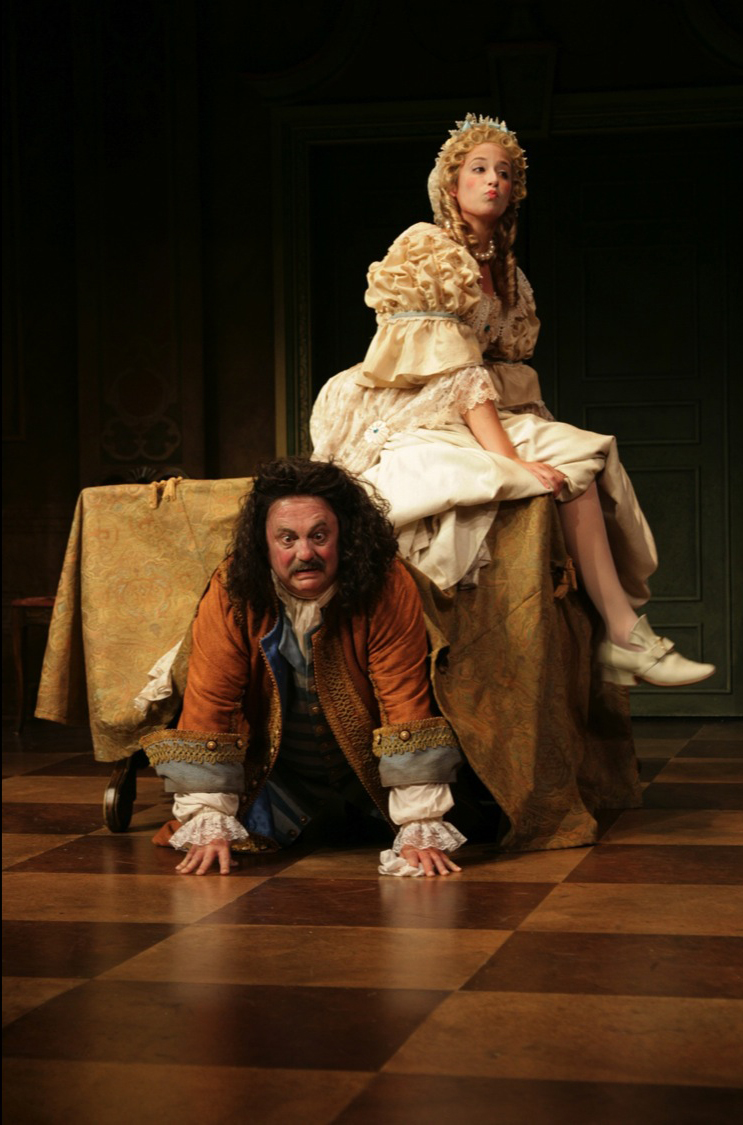
\includegraphics[width=\linewidth]{tartuffe1.jpg}
%    \caption{Exemple de costume et maquillage du théâtre français "Tartuffe"}
%
%\end{minipage}\hfill
%\begin{minipage}{0.5\textwidth}
%
%    \centering
%    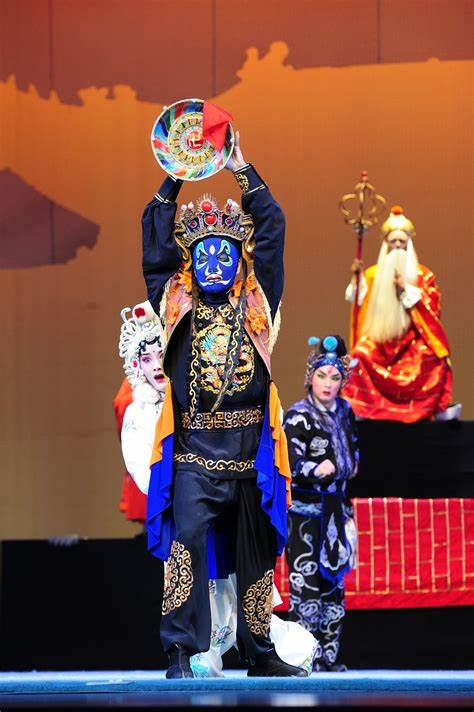
\includegraphics[width=0.97\linewidth]{chuan.jpg}
%    \caption{Exemple de costume et maquillage de l'opéra Sichuan}
%
%\end{minipage}
%\end{figure}


\begin{figure}[h!]
\centering
\raisebox{-0.5\height}{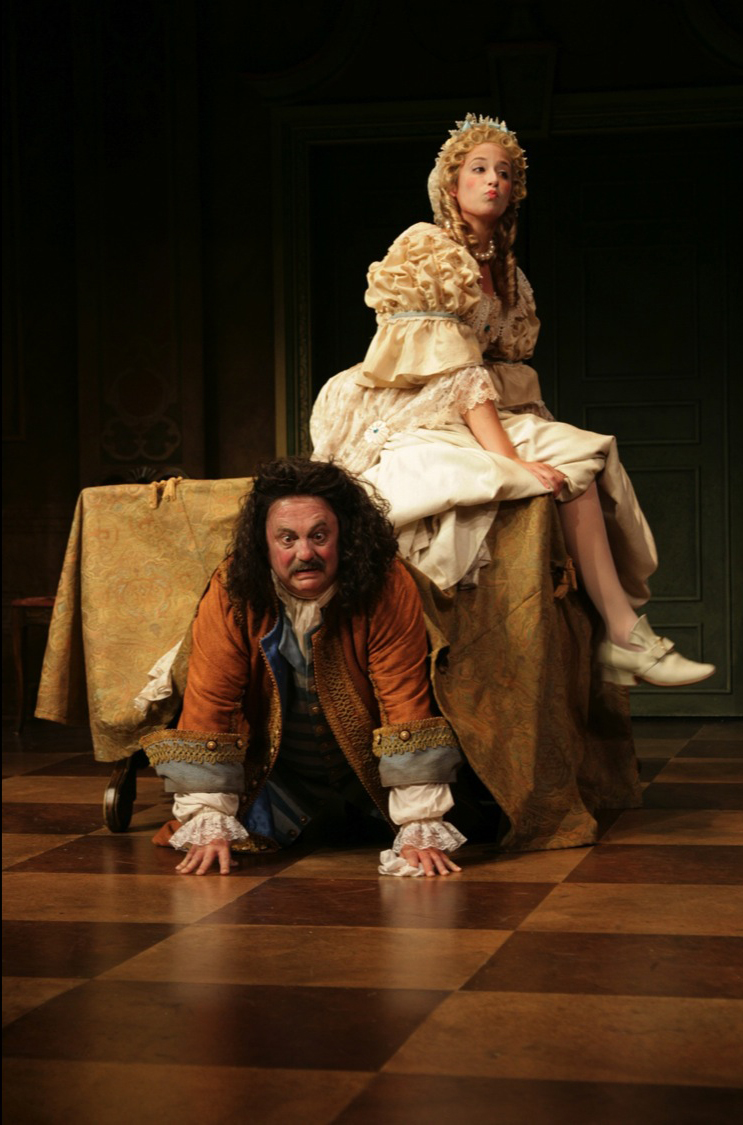
\includegraphics[width=0.45\textwidth]{tartuffe1.jpg}}%
\hspace*{0.5cm} % 控制两张图片之间的水平距离
\raisebox{-0.5\height}{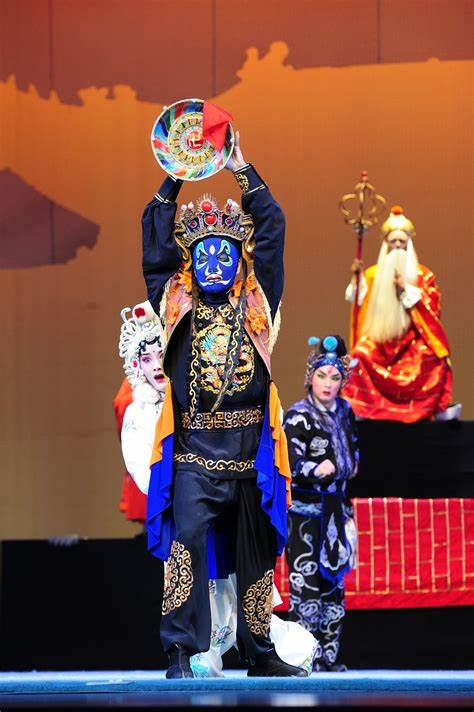
\includegraphics[width=0.45\textwidth]{chuan.jpg}}
\captionsetup{justification=centering, singlelinecheck=false}
\caption{Costume et maquillage du théâtre français ``Tartuffe" VS Costume et maquillage de l'opéra Sichuan}
\label{fig:horizontal_alignment}
\end{figure}


\subsubsection*{5. Thème}
Le théâtre français et chinois ont des thèmes différents qui reflètent leur culture et leur histoire. Le théâtre chinois a souvent des thèmes religieux et spirituels, tels que le bouddhisme, le taoïsme et le confucianisme, ainsi que des thèmes liés à la famille et à la communauté. D'autre part, le théâtre français aborde souvent des thèmes liés à l'amour et aux relations, à la politique et aux questions sociales telles que la révolution française, la lutte des classes et la corruption. Le théâtre chinois s'intéresse également à l'identité et à la culture chinoises, tandis que le théâtre français explore souvent des thèmes liés à l'identité nationale et à la diversité culturelle. 

%\subsubsection*{}
%Le théâtre français et chinois sont deux formes de théâtre très différentes avec des origines culturelles distinctes. Voici quelques différences notables entre les deux :
%
%    Histoire et traditions : Le théâtre français a une longue histoire qui remonte à l'Antiquité grecque, alors que le théâtre chinois a une histoire encore plus ancienne qui remonte à plus de 2000 ans. Les traditions et les styles de chaque forme de théâtre sont également très différents.
%
%    Styles de jeu : Le théâtre français est souvent plus réaliste et naturaliste, tandis que le théâtre chinois est plus stylisé et symbolique. Les acteurs du théâtre français cherchent souvent à reproduire le comportement et les mouvements humains de manière précise, tandis que les acteurs chinois utilisent des gestes et des mouvements symboliques pour représenter des idées abstraites.
%
%    Structure : Le théâtre français utilise souvent une structure en actes et en scènes avec des dialogues développés, tandis que le théâtre chinois utilise souvent une structure en cycles avec des transitions fluides entre les scènes. Les pièces de théâtre chinoises peuvent également incorporer des chants, des danses et des acrobaties.
%
%    Costumes et maquillage : Les costumes et le maquillage du théâtre chinois sont souvent très colorés et élaborés, tandis que ceux du théâtre français sont souvent plus simples et réalistes.
%
%    Thèmes : Les thèmes du théâtre français sont souvent centrés sur des problèmes sociaux et psychologiques, tandis que les thèmes du théâtre chinois peuvent être plus spirituels et mythiques.
%
%    Public : Enfin, le public des deux formes de théâtre peut être différent. Le théâtre français est souvent considéré comme plus intellectuel et destiné à un public plus mature, tandis que le théâtre chinois peut être plus populaire et destiné à un public plus large.
%
%Ces différences ne sont pas exhaustives et il existe bien sûr des variations à l'intérieur de chaque forme de théâtre en fonction des époques et des auteurs. Cependant, elles montrent à quel point les traditions théâtrales de ces deux cultures sont distinctes et riches en nuances.

\subsection{Similitudes entre Le Théâtre Français et Chinois}
Malgré les nombreuses différences entre les théâtres chinois et français, il existe également des points communs. Qu'il s'agisse d'opéra chinois ou de théâtre occidental, c'est un art complet composé de nombreux éléments. Les éléments de base de sa composition sont: les acteurs, les scénarios, le public et les théâtres pour les représentations théâtrales. Parmi eux, les acteurs sont les éléments de base, et les acteurs jouant les personnages de la pièce et interprétant l'intrigue de la pièce sont des conditions indispensables à l'art dramatique. L'idée de conflit dramatique et le développement d'intrigues dramatiques viennent du scénario. L'espace où le drame peut être présenté est le théâtre. Avec le théâtre, le public peut regarder les présentations des acteurs. L'émergence et l'amélioration du théâtre est un symbole de la formation et du développement du drame. Dans le théâtre, le public n'est pas seulement un apprécieur passif, mais influence aussi souvent l'effet du drame et les émotions des acteurs, ce qui devient un facteur positif pour stimuler et promouvoir le création de pièces de théâtre. Nous en énumérerons quelques-uns pour illustrer les similitudes entre le théâtre français et Chinois.
\subsubsection*{1. Importance de la Présentation Physique}
Le premier point évoque l'importance de la présentation physique dans le théâtre français et chinois. Les deux cultures ont une tradition de mouvements stylisés et exagérés pour transmettre des émotions et une signification.

Dans le théâtre français, cette importance de la physique est visible dans les techniques de jeu telles que la gestuelle, l'expression corporelle et les mouvements chorégraphiés. Les acteurs français utilisent souvent ces mouvements précis et expressifs pour communiquer l'intrigue aux spectateurs.

Dans le théâtre chinois, on pourrait le voir dans l'opéra de Pékin et le théâtre d'ombres chinois, où les acteurs utilisent ces mouvements stylisés et exagérés pour emmener les spectateurs dans l'intrigue. Les acteurs de l'opéra de Pékin sont formés à des gestes très précis, des mouvements acrobatiques et des expressions faciales exagérées pour communiquer des émotions et raconter des histoires.

Un exemple concret pour illustrer ce point pourrait être la technique de la pantomime, qui est utilisée dans les deux traditions théâtrales pour communiquer des émotions et des actions sans utiliser de paroles.

En France, la pantomime a été popularisée par Marcel Marceau, qui a créé des spectacles qui mélangeaient des mouvements physiques expressifs avec des éléments de comédie, de drame et de poésie. Dans son travail, Marceau a utilisé des gestes précis pour communiquer des émotions et raconter des histoires, souvent accompagnés de musique ou de sons pour renforcer l'effet dramatique.
En Chine, la pantomime est souvent utilisée dans le théâtre d'ombres, qui est une forme de théâtre traditionnel dans laquelle les marionnettes sont utilisées pour représenter des personnages et des scènes. Les manipulateurs de marionnettes utilisent des gestes précis pour manipuler les marionnettes, créant ainsi des mouvements et des émotions réalistes. Dans le théâtre d'ombres chinois, les mouvements des marionnettes sont souvent synchronisés avec la musique et le chant, créant ainsi une présentation cohérente et émouvante.

\begin{figure}[h!]
\centering
\raisebox{-0.5\height}{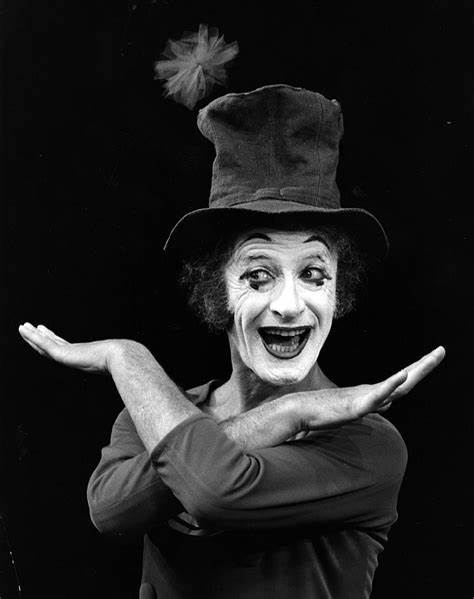
\includegraphics[width=0.49\textwidth]{marceau.jpg}}%
\hspace*{0.5cm} % 控制两张图片之间的水平距离
\raisebox{-0.5\height}{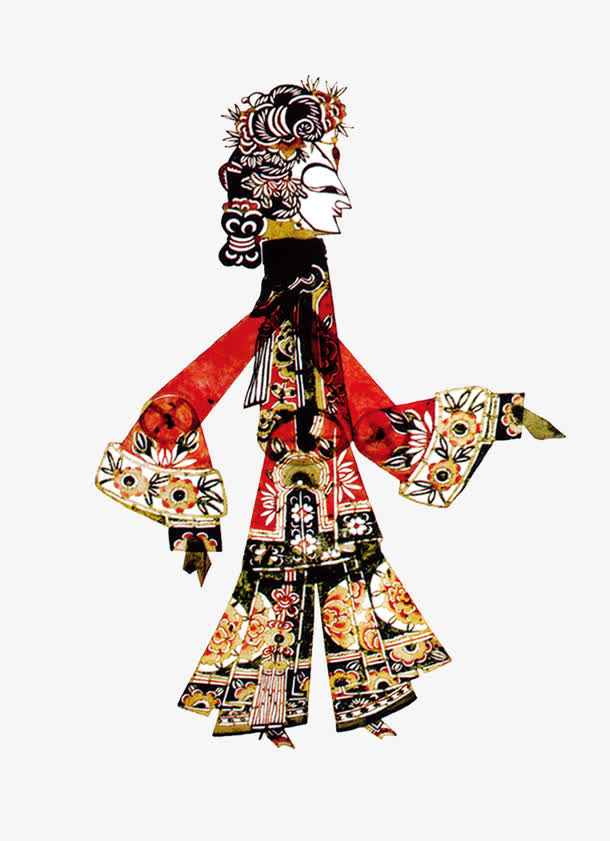
\includegraphics[width=0.45\textwidth]{piying.jpg}}
\captionsetup{justification=centering, singlelinecheck=false}
\caption{Pantomime française (Marcel Marceau, 1923-2007) VS Théâtre d'ombres (marionnettes). Ils soulignent tous les deux l'importance de la présentation physique.}

\end{figure}

\subsubsection*{2. Rôle de la Musique}
Le deuxième aspect s'agit de la musique dans le théâtre français et chinois. Les deux cultures utilisent la musique pour renforcer l'atmosphère et les émotions des pièces.

Dans le théâtre français, la musique est souvent utilisée pour créer une ambiance particulière, pour souligner l'émotion et pour renforcer l'impact des scènes dramatiques. Les comédies musicales, par exemple, intègrent des chansons pour renforcer l'intrigue et les personnages. La musique dans le théâtre français est généralement jouée par un orchestre en direct ou par des enregistrements\mycite{12}.

Dans le théâtre chinois, la musique aussi joue un rôle important. L'opéra de Pékin, par exemple, utilise une musique traditionnelle chinoise composée de percussions, de gongs, de cithares et de flûtes pour accompagner les scènes et les chants. Les acteurs sont souvent formés à chanter et à jouer d'un instrument de musique pour pouvoir se produire sur scène.

\subsubsection*{3. Importance de la Tradition}
Malgré que la tradition entre les deux pays soit très différentes, le théâtre français et chinois tous met l'accent sur la tradition et de la culture. Les deux cultures ont une riche histoire théâtrale qui influence encore aujourd'hui la production de nouvelles pièces.

Dans le théâtre français, l'influence de la tradition et de la culture est visible dans les pièces classiques qui continuent d'être produites aujourd'hui. Les œuvres de Molière, Racine et Corneille, par exemple, sont toujours étudiées et jouées régulièrement. De plus, la tradition française du théâtre de boulevard, qui met en scène des comédies légères et satiriques, reste populaire auprès des spectateurs.

Dans le théâtre chinois, la tradition et la culture sont encore plus présentes. Les pièces d'opéra de Pékin, par exemple, sont souvent basées sur des histoires de la mythologie chinoise et sont interprétées en mandarin, la langue officielle de la Chine. De plus, les costumes, la musique et les décors utilisés dans les productions sont souvent inspirés de la culture chinoise traditionnelle.

\subsubsection*{4. Utilisation de la Symbolique}
Dans le contexte du théâtre, la symbolique fait référence à l'utilisation d'objets, de costumes, de décors et de mouvements pour représenter des idées, des émotions ou des concepts abstraits. Dans le théâtre français et chinois, les artistes utilisent souvent des éléments symboliques pour communiquer des informations importantes sur l'histoire, les personnages et les thèmes de la pièce. Cela peut également aider les spectateurs à comprendre les messages et les thèmes de la pièce d'une manière plus profonde et plus significative\mycite{10}.

Dans le théâtre français, les costumes, les décors et les objets sur scène peuvent être conçus pour symboliser des éléments tels que la richesse, la pauvreté, la royauté, la guerre ou la paix. Les artistes peuvent également utiliser des symboles plus abstraits, tels que des couleurs ou des motifs spécifiques, pour transmettre des émotions ou des thèmes sous-jacents.

De même, dans le théâtre chinois, les costumes, les accessoires et les mouvements sont souvent conçus pour avoir une signification symbolique. Par exemple, les couleurs des costumes et le maquillage peuvent symboliser des aspects tels que la loyauté ou la méchanceté, et les mouvements de danse peuvent représenter des animaux ou des éléments naturels tels que le vent ou l'eau.

\begin{figure}[h!]
\centering
\raisebox{-0.48\height}{
\includegraphics[width=0.44\textwidth]{guanyu.jpg}}%
\hspace*{0.5cm} % 控制两张图片之间的水平距离
\raisebox{-0.5\height}{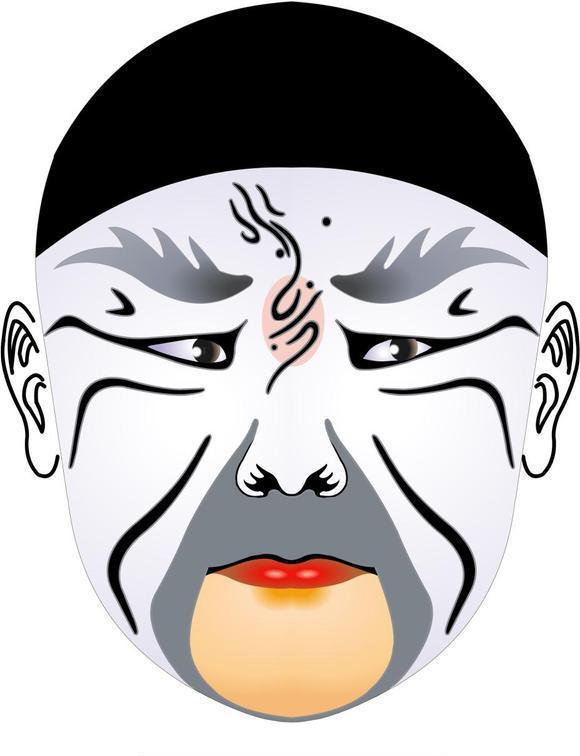
\includegraphics[width=0.49\textwidth]{zhaogao.jpg}}
\captionsetup{justification=centering, singlelinecheck=false}
\caption{Maquillage d'un personnage fidèle (Guan Yu) VS Maquillage d'un personnage méchant (Zhao Gao)}

\end{figure}

\subsubsection*{5. Importance de la Poésie}
Dans les deux cultures, la poésie est utilisée pour créer une musicalité et une rythmique particulière dans les dialogues et les monologues. Elle permet également d'exprimer des émotions et des idées complexes de manière imagée et symbolique.

Dans le théâtre français, la poésie est souvent utilisée dans les pièces classiques pour créer une harmonie entre les mots et la musique. Les dialogues et les monologues sont écrits en vers, avec une attention particulière portée à la structure et à la sonorité des phrases. Les poètes tels que Racine, Corneille et Molière ont créé des pièces de théâtre en vers qui sont devenues des classiques de la littérature française.

Dans le théâtre chinois, Les pièces telles que le Kunqu et l'opéra de Pékin, ont souvent des parties chantées en vers pour exprimer les émotions et les pensées des personnages. Les poèmes et les chants peuvent également être utilisés pour introduire les personnages et les situations, ainsi que pour créer une atmosphère particulière.

\subsubsection*{6. Analyse de la Représentation de la Société }
La représentation de la société est un élément important du théâtre français et chinois. Les deux traditions ont souvent utilisé le théâtre pour explorer les tensions et les conflits qui existent dans leur société respective.

Dans le théâtre français, la représentation de la société est souvent marquée par une certaine critique sociale. Les pièces de théâtre de Molière, par exemple, se concentrent souvent sur les éléments ridicules et absurdes de la société aristocratique française du XVIIe siècle, en utilisant l'humour et la satire pour critiquer les hiérarchies sociales et les traditions sociales qui régissaient la vie des nobles. Le théâtre français a également été un moyen pour les auteurs de mettre en avant les injustices sociales et les préjugés raciaux, comme dans les pièces de Victor Hugo.

Dans le théâtre-opéra chinois, la représentation de la société est souvent marquée par une réflexion sur les valeurs et les idéaux de la culture chinoise. Les pièces de théâtre chinoises traditionnelles utilisent souvent des personnages symboliques pour représenter différents aspects de la société chinoise, comme les mandarins, les paysans, les marchands, etc. Le théâtre chinois a également été utilisé pour célébrer les valeurs morales et les traditions culturelles de la Chine, comme dans les pièces d'opéra de Pékin.

%Dans les deux traditions théâtrales, la représentation de la société est souvent complexe et nuancée, reflétant la réalité sociale de leur époque respective. Les pièces de théâtre peuvent représenter différents aspects de la société, tels que les hiérarchies sociales, les normes culturelles, les préjugés et les conflits de pouvoir. Les personnages peuvent être utilisés pour incarner différentes perspectives et points de vue, et le public est invité à réfléchir sur ces perspectives et à en tirer des leçons.

\newpage
\fancyhead[LH]{上海交通大学学位论文}
\fancyhead[RH]{Chapitre III\quad Analyse de la Formation du Théâtre} \label{sec:3}
\section{Analyse de la Formation du Théâtre}

%Le théâtre est une forme d'art qui a évolué au fil des siècles, influencé par de nombreux facteurs, tels que la culture, l'histoire, la religion, la politique, la technologie et les événements sociaux. Voici quelques-uns des éléments qui ont influencé la formation du théâtre :
%
%La religion : Les cérémonies religieuses ont souvent inclus des éléments théâtraux, comme des chants et des danses, qui ont influencé la formation du théâtre. Par exemple, les anciens drames liturgiques européens ont évolué à partir des cérémonies religieuses chrétiennes.
%
%La politique : Le théâtre a souvent été utilisé comme un moyen de critiquer les dirigeants politiques et de faire passer des messages politiques. Par exemple, le théâtre élisabéthain en Angleterre a été influencé par la politique turbulente de l'époque et a souvent abordé des thèmes politiques dans ses pièces.
%
%La technologie : Les avancées technologiques ont eu un impact sur la formation du théâtre. Par exemple, l'invention de l'éclairage électrique a permis de nouvelles formes de spectacles théâtraux, comme les productions de Broadway à New York.
%
%Les événements sociaux : Les événements sociaux tels que les guerres, les révolutions et les mouvements sociaux ont également influencé la formation du théâtre. Par exemple, la révolution française a inspiré de nombreuses pièces de théâtre en France et a encouragé des thèmes politiques dans le théâtre.
%
%La culture et les traditions : Les cultures et les traditions ont également influencé la formation du théâtre. Par exemple, le théâtre japonais a été influencé par la culture japonaise, y compris les croyances religieuses et les pratiques artistiques traditionnelles telles que la danse et la musique.
%
%En somme, les éléments qui ont influencé la formation du théâtre sont variés et complexes, reflétant les diverses influences sociales, culturelles, politiques, religieuses et technologiques qui ont façonné cette forme d'art au fil des siècles.
\subsection{Un Exemple} \label{sec:exemple}
Dans ce chapitre, on commence par étudier un exemple du lecture erronée dans la communication théâtrale sino-française : L'orphelin de Zhao. Joseph de Prémare, un missionnaire français en Chine (1666-1736), fut le premier à traduire le drame chinois aux Européens. Joseph de Prémare était à l'origine jésuite et a reçu une bonne éducation française traditionnelle.Dans la seconde moitié de sa vie, il a eu un goût particulier pour la culture chinoise, et a traduit et étudié de nombreux classiques chinois. En 1735, le zaju des Yuan ``L'orphelin de Zhao" de Ji Junxiang, traduit par ce jésuite érudit, est publié à Paris et fait sensation\mycite{77}. Malgré la barrière de la langue et de la culture éloignée, le théâtre pourrait véhiculer des émotions universelles. 

\begin{figure}[H] 
\center{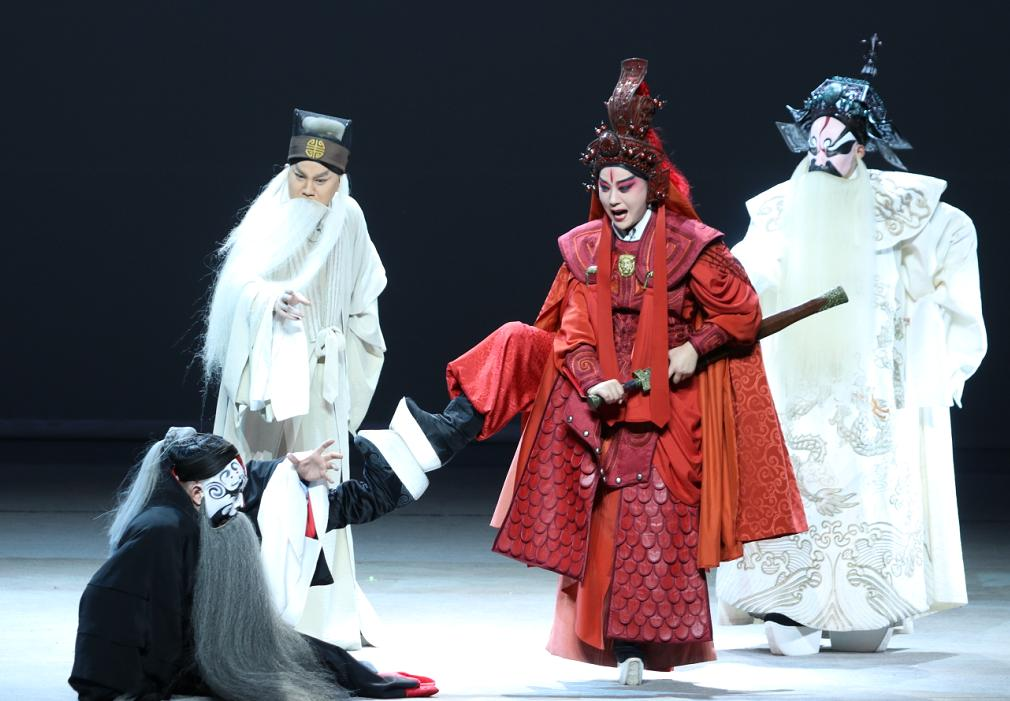
\includegraphics[width=0.9\textwidth]{zhao.png}} 
\caption{ Une scène de Kunqu ``L'orphelin de Zhao"}
\end{figure}

En tant que traducteur, Joseph de Prémare n'a pas traité ``L'orphelin de Zhao" selon le principe de la fidélité. Au contraire, il a interprété à partir du principe de l'écriture classique et a apporté de nombreuses modifications à l'original. Par exemple, pour faciliter la compréhension des lecteurs français, il a ajouté une liste de personnages qui n'existait pas dans l'original. Pour mieux s'adapter aux habitudes de lecture des Français, il a transformé cette pièce en quatre actes avec une introduction, plutôt que la forme originale de quatre actes avec une scène unique. Pour permettre aux Français de voir une pièce de théâtre chinoise qui ressemblait presque à une pièce de théâtre occidentale dans sa forme, il a également divisé chaque acte en plusieurs scènes en fonction des entrées et des sorties des personnages, en suivant les pratiques de Corneille et Racine. 

Cependant, par rapport à la façon dont Joseph de Prémare a traité les paroles de la musique dans ``L'orphelin de Zhao", toutes ces modifications semblent minimes. Le théâtre Yuan est également appelé ``théâtre de la musique et des chants" car la musique et les chants occupent une place prépondérante dans ces pièces. Pourtant, dans la traduction de Joseph de Prémare, on ne peut trouver aucune parole de musique, même après une recherche minutieuse. De plus, aucune autre forme de poésie n'est présente. La traduction littéraire est déjà difficile en soi, mais la traduction de la poésie est encore plus difficile. D'une part, la musique a des règles de métrique strictes et, d'autre part, elle est remplie d'allusions historiques. C'est pourquoi, Joseph de Prémare n'a finalement eu d'autre choix que de les résumer avec les mots ``il chante", et ainsi la pièce originale a été amputée de la plupart de son contenu.

La compréhension de Joseph de Prémare sur des chants et des vers dans la pièce des Yuan révèle le plus clairement la méconnaissance des Européens du théâtre chinois à l'époque et est un exemple typique de la mauvaise interprétation. Ce qui l'a surpris, c'est que cette pièce de Yuan n'est pas comme le théâtre occidental, où la pièce parlée et la pièce chantée sont nettement séparées, mais où le parlé et le chanté se mélangent étrangement. Plus choquant encore, non seulement les chants sont souvent interrompus par la parole, mais les acteurs peuvent aussi soudainement se mettre à chanter pendant une conversation. ``Le chant est utilisé pour exprimer des fluctuations importantes dans le cœur, comme la joie, la tristesse, la colère, le désespoir, etc. Par exemple, lorsque quelqu'un se sent indigné envers un traître, il chante ; lorsqu'un autre se prépare à se venger, il chante aussi ; et lorsqu'une personne veut mourir, elle chante encore." Quant à savoir pourquoi la version française de la pièce ``L'orphelin de Zhao" a supprimé les chants, Joseph explique : ``Certains des chants dans certaines pièces sont difficiles à comprendre, surtout pour les Européens, car ils sont remplis de choses étrangères et d'images rhétoriques que nous avons du mal à saisir, ce qui est dû à la poétique chinoise, tout comme nous avons notre propre poétique."

Pendant le siècle des Lumières, Voltaire a découvert cette pièce de théâtre chinois et en a fait une critique plus détaillée, mais il y avait encore beaucoup de malentendus. Comme ses prédécesseurs, il restait ancré dans la position classique. Il a écrit : ``L'orphelin de Zhao est un monument précieux, qui peut nous aider à comprendre l'esprit chinois mieux que tous les récits déjà écrits ou à venir sur cet empire magnifique." Cependant, en réalité, sa compréhension de l'esprit chinois n'était que dans une petite partie du théâtre chinois et ne pouvait pas représenter le panorama.

La même chose s'est produite aussi en Chine, surtout à l'époque moderne, il y a eu des interprétations erronées des œuvres d'auteurs dramatiques absurdes tels que Beckett et Eugène. Celles-ci sont étroitement liées au contexte historique et aux concepts culturels de l'époque.

Par conséquent, il est très important de comprendre l'influence de l'histoire, de la culture et d'autres facteurs sur la formation du théâtre, pour mieux apprécier cette forme d'art. On les discute dans les sections suivantes.

\subsection{Aspect Religieux}
La religion a eu une influence considérable sur la formation du théâtre à travers les âges et les cultures. Dans les sociétés primitives, le théâtre avait souvent une fonction religieuse, où les rituels et les cérémonies étaient représentés pour apaiser les dieux et assurer la fertilité des récoltes ou la victoire dans les batailles. Dans les civilisations antiques, les spectacles théâtraux étaient souvent associés aux fêtes religieuses et aux cultes des divinités. Par exemple, les tragédies grecques étaient souvent liées aux mythes et aux légendes, et avaient pour but d'explorer les thèmes de la condition humaine, de la vie après la mort et de la relation entre les mortels et les dieux.

La religion a eu une influence significative sur la formation du théâtre français, notamment pendant le Moyen Âge. Au départ, les représentations théâtrales étaient des célébrations religieuses qui avaient lieu pendant les fêtes chrétiennes, telles que la fête de Noël ou celle de Pâques. Ces représentations étaient souvent des dramatisations des histoires bibliques, jouées par des membres du clergé et des membres de la communauté locale.

Au cours de la Renaissance, les pièces de théâtre profanes ont commencé à apparaître en France, mais la religion a continué d'influencer le théâtre. Les dramaturges de la Renaissance se sont inspirés des modèles classiques grecs et romains, mais ont souvent incorporé des thèmes religieux dans leurs pièces, tels que la morale chrétienne et les allégories bibliques.

Au XVIIe siècle, la religion a continué de jouer un rôle important. Les pièces étaient soumises à la censure ecclésiastique et les dramaturges devaient souvent inclure des éléments de morale chrétienne pour éviter la répression de l'Église.

De même, la religion ont un grand impact sur la formation du théâtre chinois. L'influence de la culture bouddhiste sur le théâtre chinois est la plus évidente. Depuis la dynastie Tang, les temples bouddhistes sont devenus progressivement des lieux de représentation de théâtre. Les temples bouddhistes invitent souvent des acteurs de théâtre pour éduquer le peuple, ce qui a conduit à une influence mutuelle entre la culture bouddhiste et la culture théâtrale\mycite{00}. La conception bouddhiste de la ``rétribution des actions dans les trois vies" a été largement représentée dans le théâtre, comme dans les œuvres telles que ``L'Automne dans le palais de Han" et ``Le serpent blanc", qui présentent les thèmes de ``vies antérieures et vies présentes" et de ``cultiver pour cette vie".

De plus, la culture taoïste a également eu une certaine influence sur le théâtre chinois. Le taoïsme met l'accent sur la pensée taoïste et la conception naturaliste simple, qui se manifeste dans le théâtre par un culte de la nature et une intégration de l'art et de la nature\mycite{55}. Par exemple, ``Le pavillon aux pivoines" exprime la pensée taoïste de ``gouverner sans action" et de ``non-agir : laisser les choses venir à soi". Dans le ``Le pavillon aux pivoines", Tang Xianzu a mis en place une série de contenus liés à la culture taoïste, tels que: le thème de la vie contenu dans "Le pavillon des pivoines" est lié à la théorie de la vie dans la philosophie taoïste avec opposition aux conventions familiales et sociales comme thème principal. Et au point culminant où Du Liniang et Liu Mengmei se reconnaissent, l'auteur a également utilisé la théorie de la ``forme et de l'esprit conjointement entraînés" du taoïsme pour permettre à Du Liniang de survivre sous forme de fantôme, puis de se reconnaître et de s'unir avec Liu Mengmei. Avant que Du Liniang ne revienne à la vie, l'auteur utilise également la médecine taoïste pour décrire la pièce ``Traitement des poisons", fournissant une rationalité pour son retour à la vie.

\subsection{Aspect Historique}
%Baroque,lumière, la Révolution, la Seconde Guerre Mondiale

Les événements sociaux ont toujours eu une influence sur la formation du théâtre dans de nombreuses cultures. Par exemple, dans l'histoire française, les événements tels que la Révolution française ont conduit à l'émergence du romantisme, qui a ensuite influencé le théâtre romantique. De même, la Première Guerre mondiale a conduit à l'émergence du mouvement dadaïste, qui a eu un impact sur le théâtre absurde.

C'est aussi le même cas en Chine. Par exemple, la révolution culturelle a eu un impact sur la production théâtrale en Chine, car elle a entraîné la fermeture de nombreuses troupes et la suppression de nombreux spectacles traditionnels. Cependant, cela a également conduit à l'émergence de nouveaux styles de théâtre, tels que le théâtre de la révolution, qui ont été créés pour soutenir la propagande politique. De même, la période de la réforme économique en Chine dans les années 1980s a eu un impact sur la formation du théâtre, car elle a conduit à la création de troupes privées et à l'émergence de nouveaux styles de théâtre plus commercial.

On analyse quelques époques importantes du théâtre dans la suite pour montrer précisément comment le contexte historique influençait la formation du théâtre: 

\noindent{\textbf{Le Baroque (fin XVIe-fin XVIIe en France)}}

L'époque Baroque a été caractérisée par des conflits religieux et politiques intenses, ainsi que par une monarchie absolue et une centralisation croissante du pouvoir. Le théâtre est devenu un outil important pour le gouvernement pour promouvoir sa propagande et consolider son pouvoir, en particulier sous le règne de Louis XIV, qui a été un mécène important des arts.

Les pièces de théâtre produites à cette époque reflètent souvent les préoccupations sociales et politiques du moment, et beaucoup d'entre elles ont été conçues pour flatter et renforcer le pouvoir royal\mycite{despois1874theatre}. Les pièces de théâtre baroques ont également été marquées par une esthétique extravagante, caractérisée par des décors somptueux, des costumes élaborés et des effets spéciaux spectaculaires.

Parallèlement, les événements historiques tels que la Fronde et les conflits religieux ont également influencé le théâtre baroque en France, conduisant à l'émergence de nouveaux genres tels que la tragédie classique, qui ont cherché à refléter les valeurs et les idéaux de l'époque tout en s'inspirant des traditions dramatiques antérieures. 

\noindent{\textbf{Les Lumières (fin XVIIe-XVIIIe en France)}}

Au XVIIIe siècle, l'époque des Lumières, la montée du rationalisme et de l'esprit critique a eu un impact sur la façon dont les pièces de théâtre étaient écrites et produites. Les dramaturges de l'époque ont cherché à refléter les idées et les valeurs des Lumières dans leurs œuvres, en mettant l'accent sur la raison, la tolérance, l'éducation et la liberté.

De plus, la Révolution française a eu un impact majeur sur le théâtre français de l'époque. Les pièces de théâtre ont souvent été utilisées comme moyen de propagande politique, pour soutenir ou critiquer les événements révolutionnaires. De nombreux dramaturges se sont impliqués dans la Révolution, certains ont été emprisonnés ou exécutés, tandis que d'autres ont connu un grand succès en utilisant le théâtre pour faire passer leur message.

Enfin, l'époque des Lumières a également été marquée par l'émergence de nouveaux genres de théâtre, tels que le drame bourgeois, qui reflétait les préoccupations et les aspirations de la classe moyenne montante. Les comédies et les farces ont également continué à être populaires auprès du public, mais ont souvent été utilisées pour critiquer les élites et la noblesse.

\noindent{\textbf{Les Deux Guerres Mondiales (France)}}

La Première et la Seconde Guerre mondiale ont eu des influences significatives sur le théâtre français.
Pendant la Première Guerre mondiale, de nombreux théâtres ont fermé en raison de la mobilisation des troupes et de la crise économique qui ont suivi. Cependant, certains artistes ont continué à créer et à se produire, souvent dans des conditions difficiles. Le théâtre de guerre est également né, mettant en scène des soldats et des officiers dans des pièces de théâtre jouées sur le front. Cela a conduit à une nouvelle forme de théâtre, plus proche de la réalité et du quotidien des soldats.

La Seconde Guerre mondiale a également eu un impact majeur sur le théâtre français. Pendant l'occupation allemande, les théâtres ont été censurés et contrôlés par les autorités allemandes. Les artistes ont été persécutés en raison de leur religion, de leur race ou de leurs opinions politiques, et de nombreux théâtres ont été fermés. Certains artistes ont toutefois continué à produire des pièces clandestinement.

Après la guerre, le théâtre français a connu un renouveau avec l'avènement du théâtre de l'absurde, représenté par des auteurs tels que Samuel Beckett et Eugène Ionesco. Ces pièces ont exploré l'absurdité de la condition humaine dans un monde en mutation rapide après la guerre.

\noindent{\textbf{La Dynastie Qing (1636-1912): L'opéra de Pékin (Chine)}}

La formation de l'Opéra de Pékin est l'événement la plus important dans la dynastie Qing. À cette époque, les empereurs Kangxi, Yongzheng et Qianlong ont pris en compte les arts et la culture, et ont soutenu vigoureusement l'industrie du théâtre. La capitale est devenue le centre des arts et de la culture, les acteurs de théâtre et les troupes ont également afflué vers Beijing. Cet environnement culturel a favorisé les échanges et la fusion des genres théâtraux\mycite{15}.

D'autre part, le milieu de la dynastie Qing a connu des changements politiques et socio-économiques tels que les inondations du Jiangnan et la rébellion des Trois Feodalités, qui ont eu un certain impact sur le développement des genres théâtraux. Certains acteurs ont commencé à innover dans les formes de représentation à Beijing, fusionnant des éléments de genres théâtraux de diverses régions et y ajoutant de nouvelles techniques de présentation et des mouvements de danse, créant ainsi un nouveau genre théâtral, l'Opéra de Pékin.

En même temps, la formation de l'Opéra de Pékin est également liée à la structure sociale de l'époque. En raison du système des examens impériaux et des examens locaux de l'époque Qing, une certaine élite bureaucratique et culturelle s'est formée dans la société, qui aimait les présentations artistiques, en particulier les représentations théâtrales. L'Opéra de Pékin, en tant que nouvelle forme de représentation artistique, a été apprécié et soutenu par cette élite bureaucratique et culturelle.

\noindent{\textbf{Théâtre Moderne (Chine)}}

Le contexte historique de la formation du théâtre moderne chinois remonte à la période de changements sociaux de la fin du XIXe siècle et du début du XXe siècle en Chine. C'est une période de profonds changements économiques, politiques et culturels de la société chinoise, notamment marquée par l'établissement de la République de Chine et le déclenchement de la révolution chinoise.

Le mouvement du Nouveau Culturel est un facteur important de la promotion du développement du théâtre moderne chinois. Ce mouvement a émergé au début du XXe siècle, prônant une révolution culturelle et une libération de la pensée, et mettant l'accent sur la démocratie, la science et la modernité. Sous l'influence de ce mouvement, l'art dramatique a également commencé à se transformer en théâtre moderne, avec l'émergence d'une série d'œuvres théâtrales modernes axées sur l'innovation\mycite{16}.

En outre, la formation du théâtre moderne chinois est également liée à l'arrivée et à l'influence de la culture occidentale. Avec l'augmentation des contacts entre la Chine et l'Occident, le théâtre et les pièces de théâtre occidentaux ont été progressivement introduits en Chine, ce qui a eu une influence et une inspiration sur le théâtre chinois. Certains professionnels du théâtre chinois ont commencé à apprendre et à emprunter les techniques de création et les formes d'expression des pièces de théâtre occidentales, les fusionnant avec la culture traditionnelle chinoise pour créer un théâtre moderne chinois unique en son genre. Comme cela a été mentionné dans la section \ref{sec:exemple} de ce chapitre, bien que des malentendus puissent exister, le théâtre occidental a eu une profonde influence sur le théâtre moderne chinois.

Après la fondation de la nouvelle Chine, le théâtre chinois a connu de nombreux changements et développements. Au début des années 1950, le gouvernement chinois a commencé à mettre en œuvre des réformes socialistes, et les arts du théâtre ont également subi des transformations. Le gouvernement a fortement soutenu les arts révolutionnaires et a exigé que les œuvres théâtrales servent le peuple, reflètent l'expérience pratique et la réflexion théorique de la révolution et de la construction socialistes, et possèdent un caractère réaliste et révolutionnaire marqué\mycite{17}.

Dans ce contexte historique, le théâtre chinois moderne a connu un développement rapide. Des théâtres révolutionnaires tels que ``La fille aux cheveux blancs", ``Le port" et ``L'armée des femmes rouges", ainsi que des pièces modernes telles que ``Orage" et ``Le salon de thé", ont émergé et se sont développés sans cesse. Ces œuvres reflètent principalement les changements historiques et les problèmes de la société chinoise, tout en témoignant également du nouveau développement et de la modernisation de la culture artistique chinoise.

\begin{figure}[h!]
\centering
\raisebox{-0.5\height}{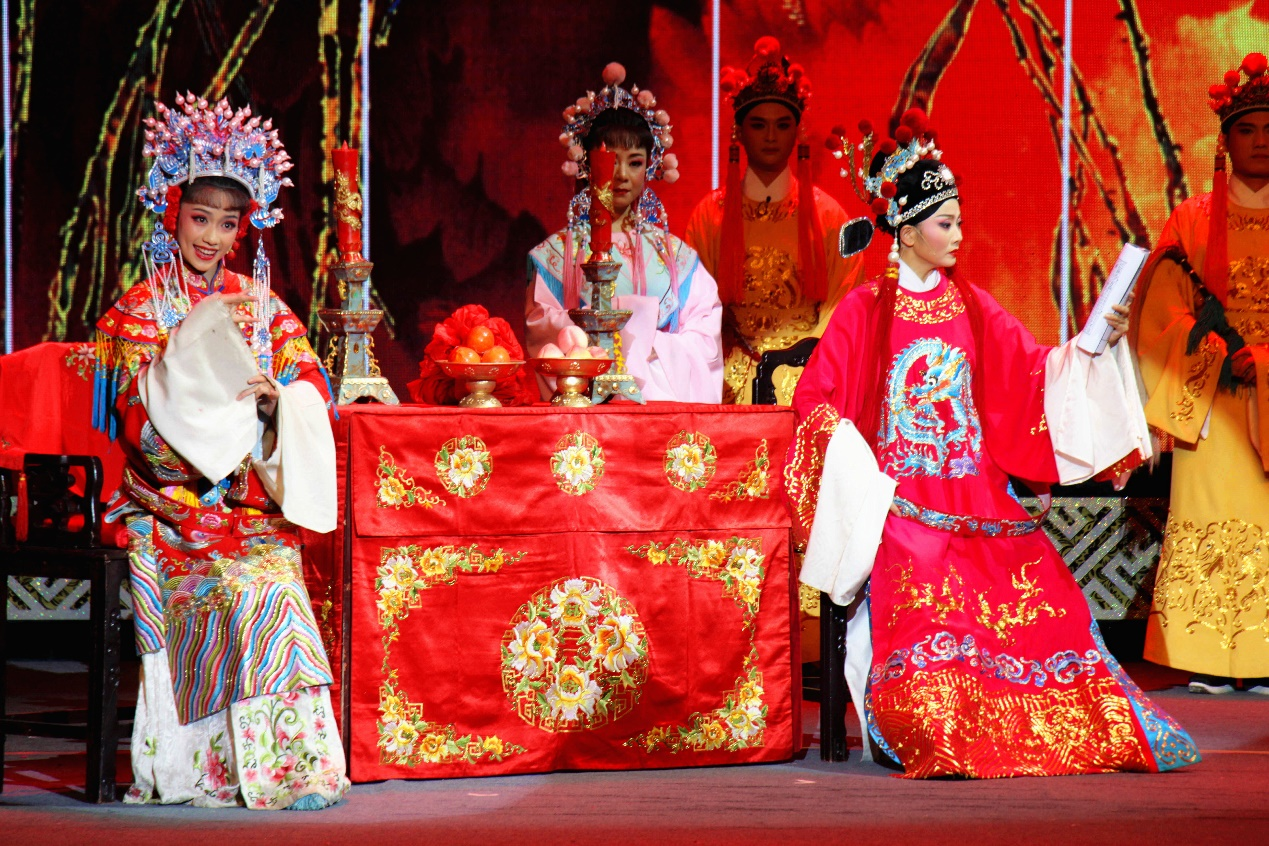
\includegraphics[width=0.45\textwidth]{fuma.jpg}}%
\hspace*{0.5cm} % 控制两张图片之间的水平距离
\raisebox{-0.5\height}{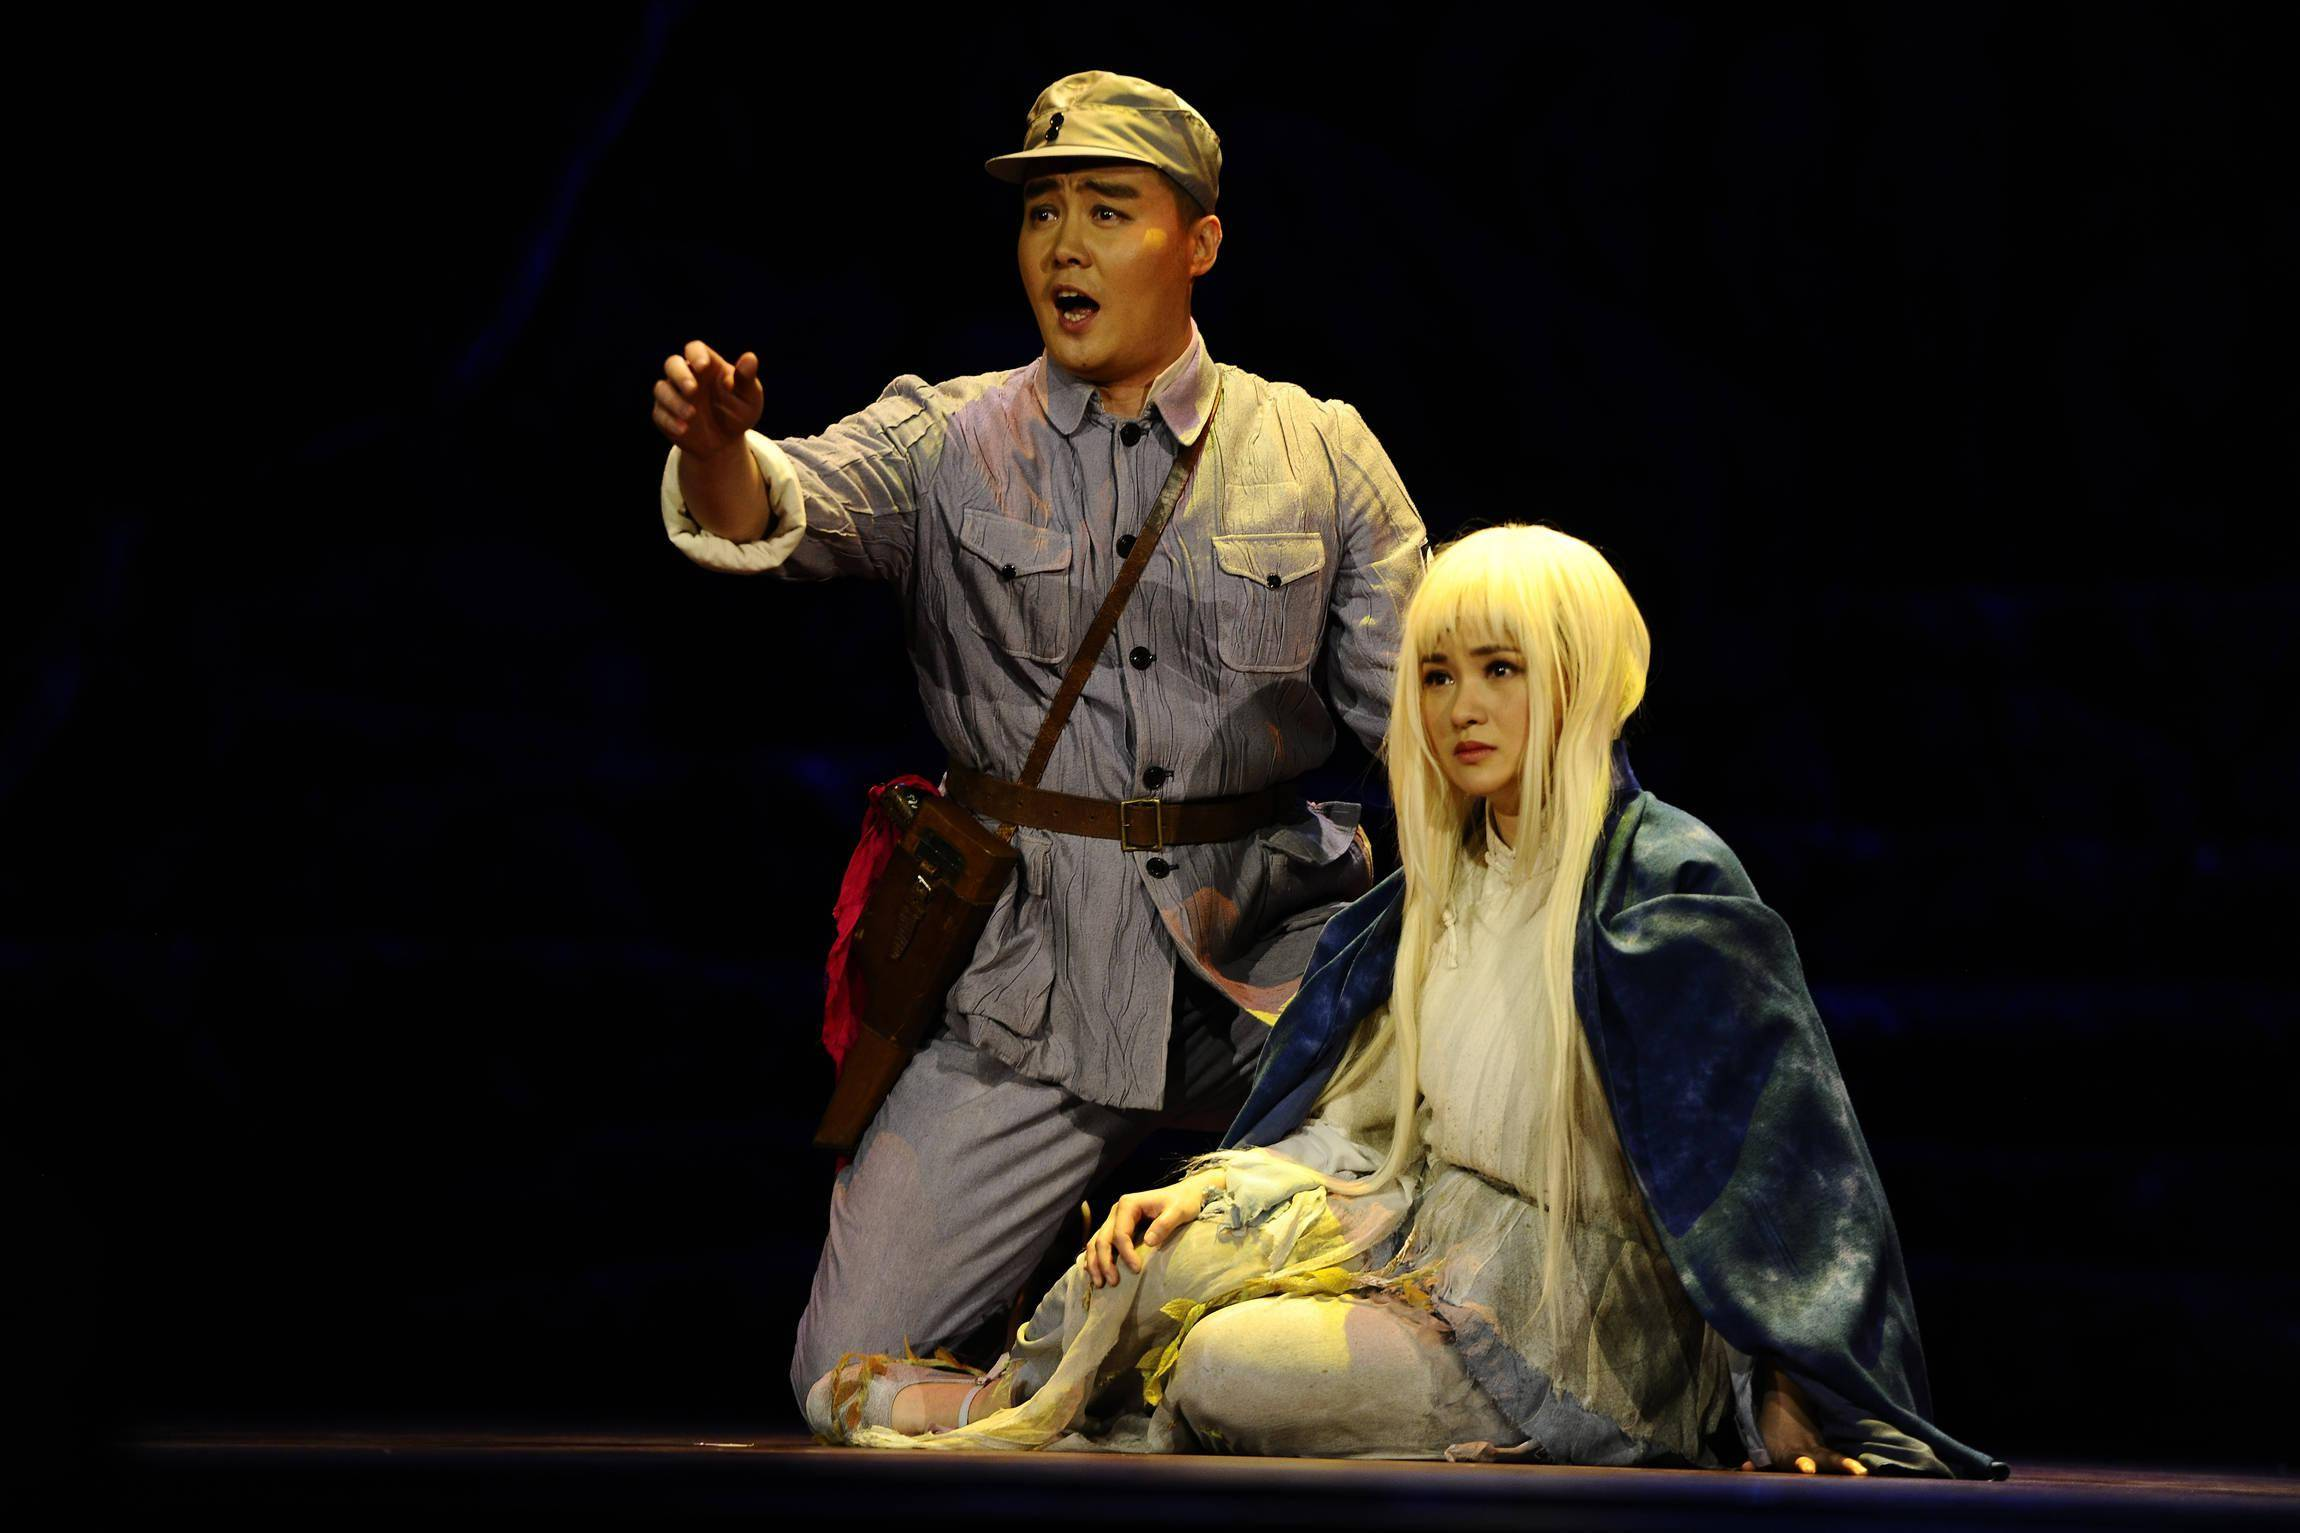
\includegraphics[width=0.45\textwidth]{baimao.jpeg}}
\captionsetup{justification=centering, singlelinecheck=false}
\caption{Théâtre traditionnel ``Mari féminin d'une princesse'' VS  Théâtre révolutionnaire ``La fille aux cheveux blancs"}

\end{figure}

La formation du théâtre chinois moderne est également liée à l'influence de l'environnement extérieur. Dans les années 1950s, la Chine a établi des relations culturelles étroites avec l'Union soviétique, et l'influence de l'art dramatique et théâtral soviétique a commencé à se manifester. De nombreux artistes du théâtre chinois ont commencé à étudier et à emprunter les techniques de création et les formes d'expression des pièces de théâtre soviétiques, apportant ainsi de nouvelles idées et styles artistiques pour le développement du théâtre chinois moderne.


\subsection{Aspect Culturel}
Tout d'abord , on liste quelques différences importantes sur les valeurs culturelles française et chinoise. La France est connue pour son individualisme, son attachement à la liberté, l'égalité, la fraternité et sa culture de la critique et du débat d'idées. La Chine, quant à elle, est souvent associée à une culture plus collective, où l'harmonie, le respect des traditions et de la hiérarchie sont des valeurs importantes. Quatre points sont distingués dessous\mycite{19}:

$\bullet$ \textbf{Individualisme vs Collectivisme}: La culture française a tendance à être plus individualiste, mettant en avant l'autonomie et la liberté individuelle. La culture chinoise, en revanche, est souvent plus collective, mettant l'accent sur la famille, la communauté et la cohésion sociale.

$\bullet$ \textbf{Hiérarchie vs Egalitarisme}: La culture française a une tradition de remise en question de l'autorité et de l'élitisme, favorisant un certain égalitarisme. La culture chinoise, en revanche, a une forte tradition de respect de la hiérarchie et des aînés, ainsi qu'un fort sens du devoir envers la famille et la société.

$\bullet$ \textbf{Plaisir vs Travail}: La culture française accorde souvent une grande importance à la qualité de vie et au plaisir de vivre. La culture chinoise, en revanche, a souvent une forte culture de travail et de persévérance, avec une forte importance accordée à l'éducation et à l'ascension sociale.

$\bullet$ \textbf{Expressivité vs Retenue}: La culture française est souvent plus expressive et démonstrative, avec une forte tradition de l'art, de la littérature et de la philosophie. La culture chinoise, en revanche, peut être plus fermée et introspective, avec une forte tradition de la méditation, de la calligraphie et de la poésie. (Cela explique bien les malentendus posés par Joseph de Prémare dans la section \ref{sec:exemple})


Comme nous l'avons illustré dans l'exemple du section \ref{sec:role}, il existe de grandes différences dans les caractérisation du rôle des théâtres chinois et français. Bien que tous deux soient des personnages classiques d'avarice, l'image de Jia Ren dans ``L'Esclave de l'argent" et celle d'Harpagon dans ``L'Avare" sont assez distinctes. Cela est principalement dû aux différences culturelles entre la Chine et la France. On l'analysera dans la partie suivante en prenant ``L'Avare" comme exemple.



La création de la littérature ancienne chinoise, y compris le zaju des Yuan, a principalement hérité de la pensée traditionnelle confucéenne et a mis l'accent sur la fonction éducative et la valeur sociale de la littérature et de l'art. Lorsque les écrivains créent des personnages, ils se concentrent toujours d'abord sur l'aspect social des personnages et semblent minimiser ou même ignorer les personnalités des personnages. Zheng Tingyu a façonné Jia Ren selon ce principe : utiliser sa plume et son encre pour montrer l'égoïsme, l'étroitesse, l'avarice, la cruauté et d'autres caractéristiques partagées par des milliers de propriétaires féodaux et de riches dans la société chinoise ancienne, de sorte que cette image est devenue un ``étranger familier". Molière a vécu au XVIIe siècle, peu après la marée haute du mouvement de la Renaissance, et la littérature humaniste produite à la Renaissance a pris la description de la réalité et la pleine manifestation de la vie comme critère de création. Ils croient que ce n'est qu'en décrivant vraiment les vraies couleurs des gens, en exprimant la nature humaine de manière vivante et éclatante et en montrant les sept émotions et les six désirs des gens, qu'ils peuvent être considérés comme vraiment respectueux des gens. Molière est un successeur exceptionnel de la littérature humaniste, s'inscrivant dans la belle tradition du réalisme dans laquelle la littérature humaniste prête attention à la vie et rend public l'individualité. Par conséquent, sa création dramatique peut prêter attention aux contradictions et aux conflits basés sur les pierres angulaires des personnages individuels de différents personnages, et s'efforcer de creuser et d'exprimer les caractéristiques de personnalité distinctives et proéminentes des personnages, ainsi que leur richesse émotionnelle intérieure complexe.

Différentes conceptions éthiques nationales conduisent également à différents comportements des personnages de la pièce. De la lamentation de l'absence d'enfant à la mendicité pour un héritier et l'achat d'un fils, le mouvement de Jia Ren contient le sens de la continuité de la lignée, de la transmission des biens de famille et de la prise en charge des personnes âgées, qui ont une forte connotation nationale. Ceci est indissociable de l'éthique traditionnelle de la nation chinoise - le confucianisme, qui a été vénéré dans les dynasties passées, prône la ``piété filiale", estime que ``la piété filiale est le fondement du pays", ``la piété filiale est la première de toutes les vertus", et accorde de l'importance à la ``chaleur, la gentillesse, le respect, l'épargne et la concession". Il a préconisé ``il y a trois types de non-piété filiale, et le plus grand est de ne pas avoir de descendants"; tout cela est devenu le modèle éthique traditionnel chinois. Ce type de concept de valeur éthique, avec le passage du temps, s'est profondément imprégné dans le sang de la nation chinoise et est devenu la norme de comportement et la norme de relations interpersonnelles. En raison de raisons sociales, historiques et politiques particulières, la France n'est pas devenue un pays avec une éthique stricte et unifiée comme la Chine. Au XIIe siècle, bien que la culture chrétienne ait dominé l'idéologie, elle s'est concentrée sur la loyauté envers le monarque et la protection de la religion, prônant la bravoure... Cependant, cela n'a été limité qu'à la petite sphère de la cour, sans s'étendre à l'ensemble du pays et sans jamais pouvoir former une norme éthique stricte et unifiée. Par conséquent, dans de nombreuses pièces de théâtre françaises, la chaîne de parenté familiale semble très fragile, facilement ébranlée par la force de l'argent et souvent confrontée à des tragédies familiales\mycite{88}.

Dans la section \ref{sec:exemple}, on pourrait aussi voir les malentendus causés par les différences culturelles, à cause de la poésie ou de la valeur. Pour mieux apprécier le théâtre d'un pays, il est essentiel de comprendre sa culture.

\subsection{Aspect Géographique}
Les conditions géographiques influencent directement le développement culturel, qui est une combinaison de facteurs historiques et culturels. La France est située en Europe occidentale, avec l'océan au sud-ouest et la mer, le transport maritime et terrestre est relativement pratique, l'industrie maritime est très développée, la communication avec les autres pays européens est très proche et les échanges commerciaux sont fréquents. Suivre la tendance du commerce a progressivement changé le style de vie social et économique de l'Europe occidentale, et a également fourni un environnement propice au libre développement des individus: la forte conscience marchande et la libération individuelle et la liberté individuelle prônées par les humanistes ont fourni à l'ego bourgeois le développement fournit un bon terreau pour le développement de la conscience de soi, l'expansion du sentiment de soi, tout l'égocentrisme et le culte de l'argent sont profondément enracinés dans le cœur des gens et deviennent un levier pour influencer les pensées et les actions des gens. Cette cupidité non seulement déforme la nature humaine, mais elle a également considérablement perturbé les relations normales entre les gens, la relation sacrée et intime entre les membres de la famille étant remplacée par l'argent. Harpagon considère l'acquisition de biens comme le seul plaisir de la vie, afin de monopoliser la propriété, il a non seulement privé ses enfants de leur droit d'héritage de leur mère décédée, mais il a également cherché à tromper ses enfants pour cacher de l'argent, et il a ardemment espéré que ses enfants mourraient tôt. Ce comportement étrange et anormal appartient précisément aux personnages qui sont influencés par l'atmosphère sociale et l'époque spécifique dans laquelle ils se trouvent, et leur comportement est le résultat logique correspondant. En revanche, la plupart des régions de la Chine sont de climat continental, avec des milliers d'années de modèle de vie agricole sur le continent, un environnement géographique semi-fermé, ce qui en fait une civilisation antique du monde fondée sur la terre et l'agriculture. La production agricole dépend principalement du climat et des saisons, avec des semis de printemps et des récoltes d'automne qui se répètent indéfiniment. Par conséquent, le noyau de la pratique esthétique des Chinois est la conscience du temps, prônant la philosophie naturelle éthique, mais il manque clairement de ``conscience marchande" de l'échange de biens. De plus, les dirigeants féodaux de toutes les dynasties en Chine, par crainte de la puissance des riches commerçants et des grosses fortunes et de leur confrontation avec les autorités, ont tous adopté une politique de ``priorité à l'agriculture et suppression de l'industrie et du commerce". Cela a largement influencé et conduit à l'orientation des valeurs du peuple chinois : mettre l'accent sur le collectif plutôt que sur les individus, mettre l'accent sur la droiture plutôt que sur le profit et prendre l'éthique comme mesure absolue de la valeur. C'est pourquoi ``L'Esclave de l'argent" ne prête pas attention à la description des caractéristiques personnelles.


\newpage
\fancyhead[LH]{上海交通大学学位论文}
\fancyhead[RH]{Chapitre IV\quad Etat Actuel du Théâtre} \label{sec:4}
\section{Etat Actuel du Théâtre en France et en Chine}

\subsection{Etat Actuel du Théâtre en France}
L'état actuel du théâtre français est dynamique et diversifié. De nos jours, le théâtre en France est représenté par une grande variété de genres, allant du théâtre classique aux productions contemporaines, en passant par le théâtre de rue, le théâtre expérimental et le théâtre musical.

Les théâtres traditionnels, tels que la Comédie-Française et l'Odéon-Théâtre de l'Europe, continuent d'attirer un public fidèle. Cependant, de nouveaux théâtres indépendants et alternatifs ont également émergé, offrant une plate-forme à des productions plus risquées et innovantes. Le théâtre français a également connu une évolution vers une plus grande diversité culturelle et linguistique, avec une représentation accrue de pièces écrites par des auteurs étrangers et des productions multilingues\mycite{sparks2014mise}.

Malgré les défis posés par la pandémie de COVID-19, le théâtre français continue de se réinventer et de trouver de nouvelles façons d'atteindre son public, notamment en utilisant des plateformes numériques pour diffuser des productions en ligne.

\subsection{Etat Actuel du Théâtre en Chine}
Le théâtre en Chine connaît actuellement une période de croissance et de diversification. Depuis l'ouverture économique de la Chine dans les années 1980s, le pays a connu une expansion rapide de culture théâtrale, avec la création de nouvelles compagnies de théâtre, la rénovation de théâtres historiques et l'organisation de festivals de théâtre internationaux. Une perspective prometteuse certes, mais uniquement dans les grandes villes. 

Le théâtre traditionnel chinois, comme l'opéra de Pékin et l'opéra de Canton, continue d'être populaire auprès du public chinois et de faire l'objet de rénovations et de mises à jour pour rester pertinent pour les générations futures. Cependant, comparée à la France, la Chine est un pays soucieux de l'héritage culturel, de sorte que la plupart des drames chinois actuels conservent les techniques artistiques et le répertoire originaux afin de perpétuer la culture chinoise ancienne\mycite{18}.

\subsection{Proposition pour la Préservation du Théâtre}
Le théâtre est un art qui a une grande importance culturelle et historique. Il reflète les coutumes, les valeurs et les croyances d'une société à travers les époques. Il est donc crucial de préserver cet art pour les générations futures.

Il est important de documenter et d'archiver les présentations théâtrales, en conservant des enregistrements vidéo ou audio, des photographies et des écrits sur les pièces de théâtre, les artistes et les compagnies de théâtre. Cette documentation peut être stockée dans des archives publiques ou privées pour que les générations futures puissent y avoir accès.

C'est aussi important de cultiver la passion pour le théâtre, c'est-à-dire d'encourager la formation des jeunes artistes dans le domaine du théâtre en offrant des formations et des ateliers de théâtre dans le programme scolaire ou extrescolaire pour les jeunes dès leur plus jeune âge: l’histoire du théâtre, des styles théâtaux chinois ou occidentaux, les métiers de la scène et du spectacle, etc. En outre, les gouvernements peuvent encourager la création de compagnies de théâtre en leur offrant des subventions et des espaces de présentation afin de garantir la carrière des acteurs et d'autres professionnels du théâtre. 

Enfin, il est crucial de soutenir et de promouvoir les pièces de théâtre auprès du public. Cela peut être fait par la programmation régulière de spectacles de théâtre dans les théâtres, les écoles, les universités et les centres communautaires, ainsi que par la promotion de la participation du public à des ateliers de théâtre et à des clubs de théâtre locaux. Oui, pour aller au théâtre, cependant, aujourd'hui, nous pouvons par ailleurs compter également sur les outils numériques pour diffuser cet art, par exemple, via des sites de streaming, les plateformes devraient rendre les pièces de théâtre plus accessibles et abordables.

\newpage
\fancyhead[LH]{上海交通大学学位论文}
\fancyhead[RH]{Conclusion}
\fancyhead[LH]{上海交通大学学位论文}
\addcontentsline{toc}{section}{Conclusion}
\section*{Conclusion}

\subsection*{Bilan: Le théâtre dans Tous Ses Etats}
La présente étude a examiné l'histoire, les similitudes et les différences du théâtre en France et en Chine, ainsi que les facteurs qui ont façonné sa formation. Le chapitre I a présenté un aperçu de l'histoire du théâtre français et chinois, en mettant en évidence les développements clés qui ont eu lieu à différentes époques. Le chapitre II a comparé les différences et les similitudes entre le théâtre français et chinois, soulignant les particularités culturelles et artistiques de chaque pays.

Le chapitre III a exploré les différents facteurs qui ont influencé la formation du théâtre, y compris les aspects religieux, historiques, culturels et géographiques. Enfin, le chapitre IV a examiné l'état actuel du théâtre en France et en Chine, et a proposé des mesures pour améliorer la conservation et la promotion du théâtre dans les deux pays.

En somme, ce mémoire a souligné l'importance de comprendre les contextes historiques, culturels et artistiques qui ont influencé le développement du théâtre en France et en Chine. Les similitudes et les différences entre ces deux traditions théâtrales ont été présentées, tout en explorant les facteurs qui ont façonné leur formation. Enfin, cette étude a proposé des mesures pour préserver et promouvoir le théâtre dans les deux pays, en tant que patrimoine culturel précieux.

\subsection*{Perspectives de Recherche}
En plus du contenu présenté dans le mémoire, il y a aussi des perspectives de recherche supplémentaires qui pourraient être explorées pour approfondir la compréhension de ces aspects. Par exemple, une analyse plus approfondie de la manière dont les avancées technologiques ont influencé l'évolution du théâtre dans chaque culture pourrait être utile. De même, une étude comparative des structures de financement du théâtre dans les deux pays et de leur impact sur la production théâtrale pourrait être envisagée. En outre, une analyse approfondie des pratiques et des tendances actuelles du théâtre dans chaque pays, telles que l'utilisation de nouvelles technologies ou l'interaction avec d'autres formes d'art, pourrait également être abordée pour fournir une perspective plus complète et actuelle sur le théâtre dans ces deux cultures.

De plus, la recherche pourrait se concentrer sur l'analyse des tendances contemporaines dans le théâtre français et chinois, en mettant en évidence les influences internationales et les développements récents. Enfin, l'étude des conditions économiques, politiques et sociales qui affectent la pratique théâtrale dans les deux pays pourrait offrir une perspective plus large sur les défis et les opportunités auxquels sont confrontés les artistes et les praticiens du théâtre. Après avoir analysé les différents aspects du théâtre, j'ose espérer que la culture théâtrale, ancienne ou contemporaine,  pourra se transmettre et se perptuer, en Chine mais aussi à l'étranger.

\newpage
\fancyhead[LH]{上海交通大学学位论文}
\fancyhead[RH]{Référence}
\addcontentsline{toc}{section}{Référence}
\section*{Référence}
\begingroup  % 去掉thebibliography环境自带的“参考文献”标题
\renewcommand{\section}[2]{}
\printbibliography
\endgroup

%\renewcommand\refname{Référence}
%\bibliography{french}

%
%\begin{figure}[htb] 
%\center{
\includegraphics[width=0.95\textwidth]  {fig2.png}} 
%\caption{内热源沿径向的分布}
%\end{figure}
%
%\begin{table}[htbp]
%\centering
%\caption{高频感应加热的基本参数}
%\begin{tabular}{c c c c}
%\toprule
%感应频率 &感应发生器功率 & 工件移动速度  &感应圈与零件间隙\\
%(KHz)&($\% \times$80Kw) &(mm/min)  &(mm)\\
%\midrule
%250 &88 &5900 &1.65\\
%
%250 &88 &5900 &1.65\\
%
%250 &88 &5900 &1.65\\
%
%250 &88 &5900 &1.65\\
%
%
%
%\bottomrule
%\end{tabular}
%\end{table}
%
%\begin{table}[htbp]
%\centering
%\captionsetup{singlelinecheck=off}
%\caption*{续表3-1}
%\begin{tabular}{c c c c}
%\toprule
%感应频率 &感应发生器功率 & 工件移动速度  &感应圈与零件间隙\\
%(KHz)&($\% \times$80Kw) &(mm/min)  &(mm)\\
%\midrule
%250 &88 &5900 &1.65\\
%
%250 &88 &5900 &1.65\\
%\bottomrule
%\end{tabular}
%\end{table}

%表格太大需要转页时,需要在续表上方注明“续表”,表头也应重复排出。

%\addcontentsline{toc}{section}{Référence}
%\renewcommand\refname{Référence}
%\begin{thebibliography}{1}
%\bibitem{1} Interplay of Eastern and Western Theatre: A Comparative Study of French and Chinese Theatres
%\bibitem{2} bbb
%\end{thebibliography}%(参考文献格式请参考GB/T 7714-2015《信息与文献 参考文献著录规则》)

%\newpage
%\fancyhead[LH]{上海交通大学学位论文}
%\fancyhead[RH]{Annexe 1}
%
%\addcontentsline{toc}{section}{附录}
%\section*{符号与标记(附录1)}
%
%\newpage
%\fancyhead[LH]{上海交通大学学位论文}
%\fancyhead[RH]{学术论文和科研成果目录}
%
%\addcontentsline{toc}{section}{攻读学位期间学术论文和科研成果目录}
%\section*{攻读学位期间学术论文和科研成果目录}
%
%[1] 张三,李四. …… (已录用)


\newpage
\begin{center}
{\listoffigures
\thispagestyle{fancy}
\fancyhead[LH]{上海交通大学学位论文}
\fancyhead[RH]{Liste des Figures}
\addcontentsline{toc}{section}{Liste des Figures}
}
\end{center}


\newpage
\fancyhead[LH]{上海交通大学学位论文}
\fancyhead[RH]{Remerciement}

\addcontentsline{toc}{section}{Remerciement}
\section*{Remerciement}

\quad \quad Tout d'abord, je voudrais adresser ma gratitude à Madame Hui-Ling PROVOST, mon professeur et ma superviseuse, pour ses conseils éclairés et sa confiance bienveillante qui m'ont permis d'accomplir ce mémoire avec succès.

Je remercie également mes parents, pour leur soutien et leur encouragements.
\hspace{8mm}


\newpage
\fancyhead[LH]{上海交通大学学位论文}
\fancyhead[RH]{}
\pagenumbering{arabic}
\heiti \section*{中法戏剧比较}%英文大摘要标题

\hspace{8mm}
\songti 戏剧是一种将文学和舞台表演与演员相结合的艺术形式,反映一个民族的文化、历史和价值观。 在法国,剧院的历史可以追溯到罗马时代,并为许多人所熟知,并在几个世纪以来发生了许多变化。 在中国,戏剧也是一门非常古老的艺术,受到许多不同文化传统的影响。 法国和中国的戏剧虽然有历史渊源,但两种艺术形式在风格、内容和技巧上都有明显差异。对中法戏剧的研究对于更好地理解这两种艺术形式之间的异同,以及促进文化之间的理解和尊重具有重要意义。 它还可以为法国和中国戏剧传统的保存和传播做出贡献,让后代能够继续欣赏这一古老的艺术。因此,本文研究的对象是中国戏剧和法国戏剧,以及它们的异同。 我们还将分析影响其形成的历史和文化背景,以及每种戏剧形式的特点和技巧。 最后,我们将结合不同的理论,考察历史和文化背景,寻求戏剧形成背后的规律。

在第一章,文章概述了法国和中国戏剧的历史。法国戏剧历史可以追溯到中世纪时期。在那个时候,戏剧表演主要是由教会组织的宗教仪式,因此被称为宗教戏剧。这些戏剧通常被表演在教堂或街头,并讲述了圣经故事或与宗教有关的主题。到了17世纪,法国戏剧经历了一个显著的变革。著名的剧作家莫里哀和里卡尔多的出现,标志着法国古典主义戏剧的兴起。这种戏剧以严格的规则和限制为特点,其目的是教育和启发观众。在18世纪,随着启蒙运动的兴起,戏剧又经历了一次变革。这一时期被称为“启蒙戏剧时代”,这种戏剧注重理性和启示,强调个人自由和独立思考。19世纪见证了许多新的戏剧形式的出现,包括现实主义和自然主义等。20世纪的法国戏剧与战争有着密切关联,产生了超现实主义戏剧、政治戏剧和荒诞主义戏剧。这个时期的剧作家包括贝克特等。中国戏剧的发展主要开始于唐朝时期,最著名的是以歌舞和音乐为主的“大曲”,随后发展出“散曲”、“小曲”等各种形式。元朝时期,由蒙古族人创立的“元曲”以及“杂剧”逐渐兴盛,与南方的戏曲交汇融合,形成了著名的元杂剧。该戏剧类型对中国戏剧产生了深远的影响,是中国戏剧发展史上的里程碑之一。关汉卿、白朴和郑廷玉等著名剧作家都身处这个时代。明清时期,中国戏曲发展到了巅峰时期,其中代表作品有“昆曲”、“京剧”、“豫剧”等。京剧是中国戏曲中最为著名的一种,于清朝末期形成,以唱、念、做、打四个基本功为主,融合了京腔、曲艺、杂技等多种元素,成为中国戏曲艺术的代表。
20世纪初期,中国戏曲遭受了西方戏剧的冲击,出现了新文化运动,对传统文化进行了激烈的批判和否定,但是同时也出现了以艺术改革为主的“昆曲革新运动”和“京剧革新运动”,使得中国戏曲在不断地更新和发展中得到了传承和延续。新中国成立后,戏曲改革更加大胆且富有政治宣传意义,服饰也发生了重大变化。如今中国戏剧正慢慢归本溯源,以继承和发扬传统戏剧文化为主要目标。

第二章探讨了法国和中国戏剧之间的差异和相似之处。中法戏剧的差异性主要体现在戏剧风格、剧本结构、人物个性、服饰妆容等。文章针对这些差异进行了详尽的分析,并对比了莫里哀的《悭吝人》与元代戏曲作家郑廷玉的《看钱奴》中吝啬鬼形象的区别,引出了中法戏剧在人物个性上的差异,并且为之后文化对于戏剧的影响分析提供了很好的例子。中法戏剧同样具有很多相似性,重点凸显在动作性、音乐和传统文化的地位、象征性以及社会性等方面。例如对于动作性,我们列举了法国的哑剧和中国的皮影戏进行对比,体现出了两种不同戏剧对于表演动作的追求。通过对中法戏剧的异同的描述和分析,以及大量的图片展示,我们对两种戏剧艺术有了更深刻的认识。

第三章分析了戏剧的形成,包括宗教、历史、文化和地理方面的因素,并结合之前章节的描述,详细解析了中法两国戏剧发展的脉络和特征形成原因。本文以中国著名戏剧《赵氏孤儿》为例,针对法国剧作家对该剧的引进和误读现象,直接体现中法戏剧在历史和文化方面的巨大差异,包括剧本结构,戏剧风格和文化运用等,并从侧面体现了多种因素对戏剧发展的影响。通过合理的对比分析,我们分别阐述了历史、文化和宗教等主导因素与戏剧发展之间的关系,得到了具有参考价值的结论,这对深入理解两国戏剧有着积极作用。比如文化因素,我们重点分析了民族价值观对于人物塑造带来的强烈影响,通过第二章《悭吝人》和《看财奴》的例子,我们不难看出中国儒家文化的集体思想,重农抑商的国家政策与法国启蒙运动带来的以人为本独立思想和资本主义浪潮所带来的截然不同的人物性格塑造,直观的展现了文化和地理因素对于戏剧发展的深刻影响。

最后一章则主要讨论了法国和中国戏剧的现状,以及为戏剧保护提出的建议。总体而言,本文突出了中法两国戏剧的丰富性和多样性,同时也探讨了两国之间的共性和差异。 通过对历史和文化因素的分析,本文对两国戏剧的形成和演变以及当今戏剧的现状提供了深刻的见解。 最后,本文强调了保护和促进戏剧作为一种重要的艺术表现形式和文化遗产的重要性。本文对期待了解中法戏剧的人提供了具有借鉴意义的资料,希望能够以此帮助促进中法文化交流与发展。 %(英文大摘要正文)



\end{document} 